%Disserta��o de Mestrado
%PPGEE - UFMG
%-------------------------------------------------------------------
%Defini��es gerais do documento
\documentclass[12pt,a4paper,titlepage,brazil,portugues,english]{book}
%--------------------------------------------------------------------
%Pacotes usados
\usepackage[brazilian]{babel}
\usepackage[latin1]{inputenc}
\usepackage[T1]{fontenc}
\usepackage{times}
%\usepackage{amssymb, amsmath, amstext} %permite simbolos matematicos
\usepackage{amsmath,amssymb,amsfonts,amstext,textcomp}
\usepackage{mathrsfs} %permite o uso de letras trabalhadas
%\usepackage{mcode}
%% Pacotes n�o implementados
% Para n�o sobrar espa�os em branco estranhos
\widowpenalty=1000 \clubpenalty=1000
\newcommand{\gepeto}[1]{\vspace*{12pt}\begin{singlespace}\hspace{2cm}\begin{small}\parbox{12cm}{#1}\end{small}\end{singlespace}\vspace*{20pt}}
%\usepackage{caligra} %letras caligraficas
%\usepackage{caligr}%letras caligraficas
%\usepackage{dsfont}%barra escura para conjuntos
\usepackage{amsthm}
\theoremstyle{definition}

\newtheorem{defi/}{Definition}[section]
\newtheorem{propo/}{Proposition}[section]
\newtheorem{coro/}{Corollary}[section]
\newtheorem{prop/}{Property}[section]
\newtheorem{lema/}{Lemma}[section]
\newtheorem{fact/}{Fact}[section]


\newenvironment{fact}
{\renewcommand{\qedsymbol}{$\square$}%
	\pushQED{\qed}\begin{fact/}}
	{\popQED\end{fact/}}

\newenvironment{lema}
{\renewcommand{\qedsymbol}{$\square$}%
	\pushQED{\qed}\begin{lema/}}
	{\popQED\end{lema/}}


\newenvironment{propo}
{\renewcommand{\qedsymbol}{$\square$}%
	\pushQED{\qed}\begin{propo/}}
	{\popQED\end{propo/}}

\newenvironment{prop}
{\renewcommand{\qedsymbol}{$\square$}%
	\pushQED{\qed}\begin{prop/}}
	{\popQED\end{prop/}}

\newtheorem{algo/}{Algorithm}[section]

\newenvironment{algo}
{\renewcommand{\qedsymbol}{$\square$}%
	\pushQED{\qed}\begin{algo/}}
	{\popQED\end{algo/}}


\newtheorem{example/}{Example}[section]

\newenvironment{example}
{\renewcommand{\qedsymbol}{$\square$}%
	\pushQED{\qed}\begin{example/}}
	{\popQED\end{example/}}



%\newtheorem{proof}{Proof}[sect/ion]
%\usepackage[dvips]{graphicx}
%\thispagestyle{empty}
%\usepackage{epsfig,latexsym}
\usepackage{graphicx}
\usepackage{float}
\usepackage{color}
\usepackage{booktabs}               % Tabelas com qualidade de publica��o
\usepackage{indentfirst}
%\usepackage{psfrag}
%\usepackage{epsfig}
\usepackage{rotating}
%fazer diagramas de blocos
\usepackage{multirow}
\usepackage{fancyhdr}
\usepackage{makeidx}
\usepackage{setspace}
%\usepackage[pdftex]{hyperref}
\usepackage[colorlinks=true, citecolor=blue]{hyperref}% tirar [colorlinks] para imprimir
%\usepackage[hang,small]{caption}
\usepackage{ae}
%\usepackage{hyperref}
\usepackage[below]{placeins}
\usepackage{flafter}
\usepackage{txfonts}
\usepackage{pxfonts}
\usepackage{natbib}
\usepackage{icomma}
\usepackage[FIGTOPCAP]{subfigure}
\usepackage{longtable}

\usepackage{icomma}

\usepackage{pdfpages}

\usepackage[left=2.5cm,right=2.5cm,top=4cm,bottom=2.5cm]{geometry}
\usepackage{appendix}

\usepackage{tabularx,ragged2e}
\renewcommand\tabularxcolumn[1]{>{\RaggedRight}p{#1}}

\newcolumntype{S}{>{\centering\arraybackslash}m{3cm}}
\newcolumntype{L}{>{\centering\arraybackslash}m{6cm}}
\newcolumntype{M}{>{\centering\arraybackslash}m{4.5cm}}

\newcolumntype{b}{X}
\newcolumntype{s}{>{\hsize=.5\hsize}X}
\raggedbottom

\usepackage{adjustbox}
\usepackage{tikz}
\usetikzlibrary{shapes.geometric, arrows, positioning, calc}

\tikzstyle{startstop} = [rectangle, rounded corners, minimum width=3cm, minimum height=1cm,text centered, draw=black, fill=red!30]
\tikzstyle{io} = [trapezium, trapezium left angle=70, trapezium right angle=110, minimum width=3cm, minimum height=1cm, text centered, draw=black, fill=blue!30]
\tikzstyle{process} = [rectangle, minimum width=3cm, minimum height=1cm, text centered, draw=black, fill=orange!30]
\tikzstyle{decision} = [diamond, minimum width=3cm, minimum height=1cm, text centered, draw=black, fill=green!30]
\tikzstyle{arrow} = [thick,->,>=stealth]

\usepackage{epigraph}
\setlength\epigraphrule{0pt}
\setlength\epigraphwidth{.4\textwidth}


\usepackage{afterpage}

\newcommand\blankpage{%
	\null
	\thispagestyle{empty}%
	\addtocounter{page}{-1}%
	\newpage}

%Modifica��es em legenda
\setlength{\belowcaptionskip}{5pt}


%--------------------------------------------------------------------
%Modifica��es em legenda (quando ocorre quebra das palavras indesejadas)
\hyphenation{na-tu-ra-is}
\hyphenation{ge-ra-do}

%--------------------------------------------------------------------
%Defini��o de comandos
\newcommand{\comment}[1]{}
\newcommand{\veq}{\vspace{0.2cm}}
\newcommand{\x}{\\[5pt]}
\newcommand{\C}[1]{\relax}

\newtheorem{teo}{Teorema}[section]
\newtheorem{defin}[teo]{Defini��o}
\newtheorem{nota}{Nota}[section]
%--------------------------------------------------------------------
%Cap�tulo personalizado
\makeatletter
\def\thickhrulefill{\leavevmode \leaders \hrule height 1ex \hfill \kern \z@}
\def\@makechapterhead#1{%
  \vspace*{10\p@}%
  {\parindent \z@ \centering \reset@font
        \thickhrulefill\quad
        \bfseries \@chapapp{} \thechapter
        \quad \thickhrulefill
        \par\nobreak
        \vspace*{10\p@}%
        \interlinepenalty\@M
        \hrule
        \vspace*{10\p@}%
        \Huge \bfseries #1\par\nobreak
        \par
        \vspace*{10\p@}%
        \hrule
    \vskip 70\p@    %100
  }}
\def\@makeschapterhead#1{%
  \vspace*{10\p@}%
  {\parindent \z@ \centering \reset@font
        \thickhrulefill
        \par\nobreak
        \vspace*{10\p@}%
        \interlinepenalty\@M
        \hrule
        \vspace*{10\p@}%
        \Huge \bfseries #1\par\nobreak
        \par
        \vspace*{10\p@}%
        \hrule
    \vskip 70\p@
 }
}

%--------------------------------------------------------------------
%Varia��o da altura da linha
\renewcommand{\baselinestretch}{1.30}

%--------------------------------------------------------------------
%Coloca Rascunho e a data
%\newcommand{\reviewtimetoday}[2]{\special{!userdict begin
%/bop-hook{gsave 20 710 translate 45 rotate 0.8 0.8 0.8 0.8 0 setcmykcolor
%/Times-Roman findfont 10 scalefont setfont 0 0   moveto (#1) show
%0 -12 moveto (#2) show grestore}def end}}
%% You can turn on or off this option.
%\reviewtimetoday{\today}{Draft Version}

%--------------------------------------------------------------------
%Criar o index
\makeindex

%--------------------------------------------------------------------
%Devido ao fancyheading
\headheight 14.7pt

%--------------------------------------------------------------------
%Trocando os efeitos da v�rgula e ponto
\DeclareMathSymbol{,}{\mathord}{letters}{"3B}
\DeclareMathSymbol{.}{\mathpunct}{letters}{"3A}


\setlength{\marginparwidth}{2cm}

\usepackage{lipsum}  
\usepackage{xargs}
\usepackage[colorinlistoftodos,textsize=scriptsize]{todonotes}
\newcommand{\duvida}[1]{\todo[color=green!40]{#1}}

\usepackage{tikz}
\usepackage{tikz-qtree}

\usetikzlibrary{trees}
\usepackage{adjustbox}
%
%\usepackage{subfig}/
%\usepackage{graphicx}


\begin{document}
%--------------------------------------------------------------------
%P�gina em algarismos romanos
\pagenumbering{roman}
\selectlanguage{english}

%--------------------------------------------------------------------
%Capa
%CAPA
\begin{titlepage}

%Filia��o
%--------------------------------------------------------------------
\begin{figure}[!ht]
\begin{minipage}[b]{0.7\linewidth}
\begin{tiny}
Modeling, Analysis and Control of Nonlinear Systems Laboratory \\
Electronics Engineering Department \\
Federal University of Minas Gerais\\
Av. Ant�nio Carlos 6627, 31270-901 Belo Horizonte, MG Brasil\\
Phone: +55 3499-4866 - Fax: +55 3499-4850 %\\

\end{tiny}
\end{minipage}\hfill
\begin{minipage}[c]{0.3\linewidth}
\begin{flushright}
\vspace{-1.2cm}
\includegraphics[scale=1.37]{Imagens/mac.png}
\end{flushright}
\end{minipage}
\end{figure}
%--------------------------------------------------------------------

%T�tulo
%--------------------------------------------------------------------
\vspace{1.75cm}
\begin{center}
\thickhrulefill
\par\nobreak
\vspace*{10\p@}%
\hrule
\vspace*{10\p@}%
{\bf \Huge \bfseries  Sensor Fusion \\}
\vspace{0.25cm}
{\bf \Huge \bfseries  for Irregularly Sampled Systems}
\vspace*{10\p@}%
\hrule
\vspace*{40\p@}%
%--------------------------------------------------------------------

%Autor
%--------------------------------------------------------------------
{\large \bf Taiguara Melo Tupinamb�s}\\[0.5cm]
\end{center}
%--------------------------------------------------------------------


%Descri��o
%--------------------------------------------------------------------
\vspace{1.75cm}
\begin{flushright}
\begin{minipage}{0.7\linewidth}
Master Dissertation submitted to the Graduate Program in Electrical Engineering of the School of Engineering of the Federal University of Minas Gerais in partial fulfillment of the requirements for the Master's Degree in Electrical Engineering.\\
\end{minipage}
\end{flushright}
\vspace{1.6cm}


%--------------------------------------------------------------------

%Orienta��o
%--------------------------------------------------------------------
\begin{tabular}{ll}
  {\bf Advisors:} & Prof. Bruno Ot�vio Soares Teixeira, Dr.\\
    &                        Prof. Leonardo Ant�nio Borges T�rres, Dr.\\
\end{tabular}
\vspace{1.6cm}

%--------------------------------------------------------------------
%Cidade e Data
%--------------------------------------------------------------------
\centerline{Belo Horizonte, February, 2019}
%--------------------------------------------------------------------
\end{titlepage}

\clearpage
\thispagestyle{empty}
\cleardoublepage
\includepdf[pages=-]{folha_rosto.pdf}
\includepdf[pages=-]{ficha_catalografica.pdf}
\includepdf[pages=-]{folha_numero.pdf}
%%CAPA
\begin{titlepage}

%Filia��o
%--------------------------------------------------------------------
\begin{figure}[!ht]
\begin{minipage}[b]{0.7\linewidth}
\begin{tiny}
Modeling, Analysis and Control of Nonlinear Systems Laboratory \\
Electronics Engineering Department \\
Federal University of Minas Gerais\\
Av. Ant�nio Carlos 6627, 31270-901 Belo Horizonte, MG Brasil\\
Phone: +55 3499-4866 - Fax: +55 3499-4850 %\\

\end{tiny}
\end{minipage}\hfill
\begin{minipage}[c]{0.3\linewidth}
\begin{flushright}
\vspace{-1.2cm}
\includegraphics[scale=1.37]{Imagens/mac.png}
\end{flushright}
\end{minipage}
\end{figure}
%--------------------------------------------------------------------

%T�tulo
%--------------------------------------------------------------------
\vspace{1.75cm}
\begin{center}
\thickhrulefill
\par\nobreak
\vspace*{10\p@}%
\hrule
\vspace*{10\p@}%
{\bf \Huge \bfseries  Sensor Fusion \\}
\vspace{0.25cm}
{\bf \Huge \bfseries  for Irregularly Sampled Systems}
\vspace*{10\p@}%
\hrule
\vspace*{40\p@}%
%--------------------------------------------------------------------

%Autor
%--------------------------------------------------------------------
{\large \bf Taiguara Melo Tupinamb�s}\\[0.5cm]
\end{center}
%--------------------------------------------------------------------


%Descri��o
%--------------------------------------------------------------------
\vspace{1.75cm}
\begin{flushright}
\begin{minipage}{0.7\linewidth}
Master Dissertation submitted to the Graduate Program in Electrical Engineering of the School of Engineering of the Federal University of Minas Gerais in partial fulfillment of the requirements for the Master's Degree in Electrical Engineering.\\
\end{minipage}
\end{flushright}
\vspace{1.6cm}


%--------------------------------------------------------------------

%Orienta��o
%--------------------------------------------------------------------
\begin{tabular}{ll}
  {\bf Advisors:} & Prof. Bruno Ot�vio Soares Teixeira, Dr.\\
    &                        Prof. Leonardo Ant�nio Borges T�rres, Dr.\\
\end{tabular}
\vspace{1.6cm}

%--------------------------------------------------------------------
%Cidade e Data
%--------------------------------------------------------------------
\centerline{Belo Horizonte, February, 2019}
%--------------------------------------------------------------------
\end{titlepage}

\clearpage
\thispagestyle{empty}
\cleardoublepage

%%--------------------------------------------------------------------
%
%%--------------------------------------------------------------------
%%Dedicat�ria
%\chapter*{Dedicat�ria}

\vspace{5cm}
\begin{flushright}
\begin{minipage}{0.7\linewidth}
\emph{A minha querida esposa Anny, que com sua dedica��o e seu amor incondicional me faz sorrir, mesmo nas horas mais dif�ceis.}\\
\end{minipage}
\end{flushright}

%\clearpage
%\thispagestyle{empty}
%\cleardoublepage
%%--------------------------------------------------------------------
%
%
%%--------------------------------------------------------------------
%Agradecimentos
\chapter*{Agradecimentos}

Antes de tudo, sou grato � UFMG por ter me proporcionado toda uma estrutura de excel�ncia, para a realiza��o dos meus estudos. � atrav�s de institui��es p�blicas de ensino superior como ela que podemos evoluir como sociedade. Estendo meus agradecimentos ao PPGEE-UFMG e aos seus funcion�rios, professores e alunos que contribuiram para o desenvolvimento deste trabalho. E ao CNPq, pelo apoio financeiro durante grande parte do meu mestrado.

Agrade�o aos meus orientadores, Prof. Bruno Teixeira e Prof. Leonardo T�rres, por todo o ensinamento e pela forma contagiante com que compartilham suas experi�ncias. Serei eternamente grato por terem me acolhido de volta � Academia, ap�s longos anos.

Aos amigos do Laborat�rio de Modelagem, An�lise e Controle de Sistemas N�o-Lineares (MACSIN), pelo companheirismo e apoio. Aprender junto com voc�s foi incr�vel.

Tamb�m tenho muito a agradecer � equipe do Laborat�rio de Nanoespectroscopia (LabNS), � qual me juntei recentemente, e que tem renovado de forma constante a minha paix�o pela ci�ncia.

�s amigas e aos amigos do Bloco Pr�-Sal, por trazerem leveza e alegria � minha vida, al�m de serem modelos exemplares que tenho para a vida. � turma de gradua��o da El�trica, em especial ao Igor Baratta, grande amigo e conselheiro. 

Termino esses agradecimentos, mencionando aqueles sem os quais nada faria sentido nem seria poss�vel. Aos meus pais, Marilu e Ubiratan, � minha irm� e ao seu marido, Moara e Matheus, agrade�o imensamente pela forma��o, pela confian�a, pelos conselhos e pelo amor incondicional. Voc�s me fazem muito feliz. Aos meus sobrinhos, Iara e Cau�, pelo carinho e pela inspira��o. � minha amada esposa Marina, meu porto seguro. Voc� me faz ser uma pessoa melhor todo dia. E �s minhas fam�lias Melo e Tupinamb�s, pelo amor e pelo incentivo constantes.
\\

\clearpage
\thispagestyle{empty}
\cleardoublepage
%%--------------------------------------------------------------------
%
%
%%--------------------------------------------------------------------
%Ep�grafe
\chapter*{Ep�grafe}

\begin{flushright}
\begin{minipage}{0.7\linewidth}
\emph{``Ele vos deu vida, estando v�s mortos nos vossos delitos e pecados.\\
Nos quais andastes outrora, segundo o curso deste mundo, segundo o
pr�ncipe da potestade do ar, do esp�rito que agora atua nos filhos
da desobedi�ncia.\\
Entre os quais tamb�m todos n�s andamos outrora, segundo as
inclina��es da nossa carne, fazendo a vontade da carne e dos
pensamentos; e �ramos, por
natureza, filhos da ira, como tamb�m os demais.\\
Mas Deus, sendo rico em miseric�rdia, por causa do grande amor com
que nos amou,\\
E estando n�s mortos em nossos delitos, nos deu vida juntamente
com Cristo - pela gra�a sois salvos,\\
E, juntamente com ele, nos ressuscitou, e nos fez assentar nos
lugares celestiais em Cristo Jesus;\\
Para mostrar, nos s�culos vindouros, a suprema riqueza da sua
gra�a, em bondade para conosco, em Cristo Jesus.\\
Porque pela gra�a sois salvos, mediante a f�; e isto n�o vem de
v�s, � dom de Deus.\\
N�o vem das obras, para que ningu�m se glorie;\\
Pois somos feitura dele, criados em Cristo Jesus para boas obras, as
quais Deus de antem�o preparou para que and�ssemos nelas.''\\}
\end{minipage}
\end{flushright}
%\vspace{3cm}
\begin{flushright}
{Ef 2:1-10}
\end{flushright}

\clearpage
\thispagestyle{empty}
\cleardoublepage
%%--------------------------------------------------------------------


%%--------------------------------------------------------------------
%Sum�rio
\pagestyle{myheadings}
\begin{spacing}{1.5}
\tableofcontents
\end{spacing}
\thispagestyle{empty}
\cleardoublepage

%%
%%%--------------------------------------------------------------------
%Resumo
\begin{spacing}{1}
\chapter*{Resumo}
\addcontentsline{toc}{chapter}{Resumo}

\vspace{-2cm} O uso de v�rios sensores  para melhorar a qualidade na informa��o obtida pelos dados tem crescido de forma cont�nua nas �ltimas d�cadas. Com os avan�os em tecnologia de microprocessadores e dispositivos de comunica��o, redes de sensores continuar�o a crescer em tamanho e complexidade. As aplica��es mais populares para combinar dados de m�ltiplos sensores est�o relacionadas a estima��o de estados de um sistema din�mico. Para isso, duas fontes ruidosas de informa��o s�o necess�rias: um modelo de processo, que descreve como os estados evoluem no tempo; e um modelo de observa��o, cujos dados geralmente prov�m de sensores. Como a maioria dos sensores s�o digitais, os sinais devem ser amostrados para que possam ser processados, dando origem aos sistemas amostrados. Estimadores de estado cl�ssicos, como o famoso filtro de Kalman, consideram que o processo de amostragem adv�m de um amostrador ideal. Ou seja, a fonte de informa��o transmite dados em intervalos de tempo regularmente espa�ados. Sob tais considera��es, sistemas cont�nuos podem ser discretizados em representa��es invariantes no tempo, na maioria dos casos. No entanto, devido ao cada vez mais comum uso de complexas redes de sensor sem sincroniza��o temporal, muitas aplica��es n�o podem depender de dados transmitidos de forma regular. Existem adapta��es aos m�todos de estima��o de estados para lidar com a maioria das irregularidades, desde que os carimbos de tempo sejam parte do pacote de medi��o e que o aumento no custo computacional seja aceit�vel. Caso o carimbo de tempo n�o possa ser utilizado no processo de estima��o, pode-se investir em sincroniza��o dos dados ou assimilar as informa��es em instantes de tempo incorretos. Os efeitos no desempenho da estima��o da �ltima abordagem ainda � pouco estudada. Desta forma, nosso trabalho investiga como o desempenho � deteriorado ao negligenciar os carimbos de tempo das medi��es em algoritmos de estima��o de estados. N�s consideramos o processo de Poisson como modelo para gerar a sequ�ncia de instantes de tempo irregular, e estudamos os erros introduzidos pelo deslocamento no tempo das amostras do sinal. Ent�o, n�s simulamos os resultados de estima��o para um sistema linear e outro n�o-linear, com amostragem n�o peri�dica, utilizando o filtro de Kalman para o caso linear e sua varia��o \textit{unscented} para o caso n�o-linear. Algoritmos s�o implementados tanto para utilizar o carimbo de tempos no processo de estima��o quanto para negligenci�-los, e os resultados de v�rias realiza��es s�o comparados para diferentes cen�rios de simula��o. Observamos situa��es em que o desempenho dos dois algoritmos varia de forma significativa e outras em que n�o h� nenhuma diferen�a estat�stica.
\\ \\
\textbf{Keywords:} Fus�o Sensorial; Amostragem Irregular; Estima��o de Estados; Sistemas Amostrados; Carimbo de Tempo.

\clearpage
\thispagestyle{empty}
\cleardoublepage
%%--------------------------------------------------------------------
%
%%--------------------------------------------------------------------
%Abstract
\chapter*{Abstract}
\addcontentsline{toc}{chapter}{Abstract}

\vspace{-2cm} 
The use of multiple sensors to improve data quality has grown continuously over the last few decades. With the never-ending advances in technology of microprocessors and communication devices, sensor networks will continue to increase in both size and complexity. The most popular applications for fusing data from various sources are related to estimating the states of a dynamic system. For that, two noisy sources of information are needed: a process model that describes how the states evolve in time; and an observation model, whose data are usually obtained from sensors. Since most sensors are digital, signals must be sampled in order to be processed, leading to sampled-data systems. Classical state estimators in these cases, like the well-known Kalman filter, implicitly consider regularly sampled signals with constant time intervals between samples, such that continuous-time systems can be time discretized into time-invariant representations in most cases. However, because of the widespread use of complex sensor networks without explicit time synchronization, many applications cannot rely on data being transmitted regularly. There are adaptations to state estimation techniques that handle most of the irregularities, provided that timestamps are part of measurement packets and that the increase in computational processing time is acceptable. If timestamps cannot be used in the estimation process, one can either invest in synchronization or accept the assimilation of information at incorrect time instants. The effects in estimation performance of the latter approach has not yet been extensively studied. In this work we investigate how performance is deteriorated by neglecting measurements timestamps in state estimation algorithms. We consider the Poisson process as a model to generate the irregular time instants sequences, and we assess state estimation results for linear and nonlinear systems simulated with aperiodic sampling, using the Kalman filter for the former and its adapted unscented version for the latter. Algorithms are designed to use timestamps or to neglect them in the estimation process, and their results over multiple runs are compared for different simulation scenarios. Finally, we identify and discuss relations between different sets of parameters, such as signal-to-noise ratios and average sampling frequencies, and the degradation in performance.
\\ \\
\textbf{Keywords:} Sensor Fusion; Irregular Sampling; State Estimation; Sampled-data Systems; Time Synchronization; Time-Stamp.

\clearpage
\thispagestyle{empty}
\cleardoublepage
\end{spacing}
%%%--------------------------------------------------------------------
%%
%%%--------------------------------------------------------------------
%%%Lista de figuras
\begin{sloppypar}
\listoffigures
\end{sloppypar}
\addcontentsline{toc}{chapter}{List of Figures}
\clearpage
\thispagestyle{empty}
\cleardoublepage
%%
%%%--------------------------------------------------------------------
%%%Lista de Tabelas

\listoftables
\addcontentsline{toc}{chapter}{List of Tables}
\clearpage
\thispagestyle{empty}
\cleardoublepage

%
%%%--------------------------------------------------------------------
%%%S�mbolos
%%%--------------------------------------------------------------------
\chapter*{List of Symbols and Acronyms}
\addcontentsline{toc}{chapter}{List of Symbols and Acronyms}
%\vspace{-2.0cm}
\section*{Symbols}

\subsection*{Chapter 1}

\begin{longtable}{ll}
$\mathbb{N}^+$			& positive integers; \\
$\mathbb{R}$			& real numbers; \\
$\mathbb{R}^n$			& $\mathbb{R}^{nx1}$ $n$-dimensional Euclidean space; \\

$\forall$				& for all; \\
$\in$					& belongs to; \\
$>$						& greater than; \\
$<$						& less than; \\
$\geq$					& greater than or equal to; \\
$\leq$					& less than or equal to; \\
$\triangleq$			& equals by definition; \\	
$\approx$				& approximately equal to; \\
$\sim$					& is distributed as; \\

$\mathcal{N}$			& Gaussian distribution; \\
$\mathcal{E}$			& Exponential distribution; \\
$x_i$					& $i$th entry of x; \\	

$f$						& process model; \\
$g$						& observation model; \\
$t$						& continuous-time index; \\
$k$						& discrete-time index of measurements; \\
$i$						& discrete-time index of input; \\
$t_k$					& continuous-time sampled instants; \\
$T$						& input sampling interval; \\
$x(t)$					& state vector; \\
$x(t_k)$				& state vector at continuous-time sampled instants; \\
$u(t)$					& input vector; \\
$u(iT)$					& input vector at continuous-time sampled at time $t = iT$; \\						
$w(t)$					& process noise vector; \\
$y_{t_k}$            	& output vector at continuous-time sampled instants;\\
$\delta_{k}$			& measurements time-delay; \\
$v(t_k)$				& measurement noise vector; \\
$h_k$					& time intervals between two continuous-time sampled instants; \\
$\lambda$ 				& parameter of the exponential distribution; \\
$\lambda_h$				& parameter of the exponentially distributed random variable $h_k$; \\
$\lambda_{\delta_{k}}$	& parameter of the exponentially distributed random variable $\delta_{k}$; \\
$N$						& amount of identical sensors in the sampling model; \\
$L$						& sampling period of the identical sensors in the sampling model; \\
$P$						& covariance matrix; \\
$\alpha$				& relation between output (expected) and input sampling time intervals . \\
\end{longtable}

\subsection*{Chapter 2}


\begin{longtable}{ll}
	$\mathbb{N}^+$			& positive integers; \\
	$\mathbb{R}$			& real numbers; \\
	$\mathbb{R}^n$			& $\mathbb{R}^{nx1}$ $n$-dimensional Euclidean space; \\
	
	$\forall$				& for all; \\
	$\in$					& belongs to; \\
	$>$						& greater than; \\
	$<$						& less than; \\
	$\geq$					& greater than or equal to; \\
	$\leq$					& less than or equal to; \\
	$\triangleq$			& equals by definition; \\	
	$\approx$				& approximately equal to; \\
	$\sim$					& is distributed as; \\
	
	$\mathcal{N}$			& Gaussian distribution; \\
	$\mathcal{E}$			& Exponential distribution; \\
	$x_i$					& $i$th entry of x; \\	
	
	$f$						& process model; \\
	$g$						& observation model; \\
	$t$						& continuous-time index; \\
	$k$						& discrete-time index of measurements; \\
	$i$						& discrete-time index of input; \\
	$t_k$					& continuous-time sampled instants; \\
	$T$						& input sampling interval; \\
	$x(t)$					& state vector; \\
	$x(t_k)$				& state vector at continuous-time sampled instants; \\
	$u(t)$					& input vector; \\
	$u(iT)$					& input vector at continuous-time sampled at time $t = iT$; \\						
	$w(t)$					& process noise vector; \\
	$y_{t_k}$            	& output vector at continuous-time sampled instants;\\
	$\delta_{k}$			& measurements time-delay; \\
	$v(t_k)$				& measurement noise vector; \\
	$h_k$					& time intervals between two continuous-time sampled instants; \\
	$\lambda$ 				& parameter of the exponential distribution; \\
	$\lambda_h$				& parameter of the exponentially distributed random variable $h_k$; \\
	$\lambda_{\delta_{k}}$	& parameter of the exponentially distributed random variable $\delta_{k}$; \\
	$N$						& amount of identical sensors in the sampling model; \\
	$L$						& sampling period of the identical sensors in the sampling model; \\
	$P$						& covariance matrix; \\
	$\alpha$				& relation between output (expected) and input sampling time intervals . \\
\end{longtable}


\subsection*{Chapter 3}

\subsection*{Chapter 4}

\subsection*{Chapter 5}

\newpage
\section*{Acronyms}
\begin{tabular}{ll}
	CDF			& Cumulative Distribution Function; \\
	DAI			& Data In; \\
	DAO			& Data Out; \\
	DEI			& Decision In; \\
	DEO 		& Decision Out; \\
	DSET 		& Dempster-Shafer Evidence Theory; \\		
	EKF			& Extended Kalman Filter; \\
	FEI			& Feature In; \\
	FEO			& Feature Out; \\
	KF 			& Kalman Filter; \\
	MOP 		& Measures Of Performance; \\
	NMR 		& Nuclear Magnetic Resonance; \\
	NUS 		& Non-Uniform Sampling; \\ 
	OOSM 		& Out-Of-Sequence Measurement; \\
	PDF         & Probability Distribution Function; \\
	PF 			& Particle Filter; \\
	RMSE		& Root Mean Square Error; \\
	SOD			& Send-On-Delta; \\
	SNR			& Signal-to-Noise Ratio; \\
	TDS			& Time-Delay System; \\
	UKF			& Unscented Kalman Filter; \\
\end{tabular}


\clearpage
\thispagestyle{empty}
\cleardoublepage
\normalsize
%%%%--------------------------------------------------------------------
%%%
%%%%Abreviaturas
%%%%%--------------------------------------------------------------------
%\chapter*{Lista de Acr�nimos}
\addcontentsline{toc}{chapter}{Lista de Acr�nimos}

\vspace{-2.0cm}

\footnotesize
\begin{tabular}{ll}
AIC                      & Crit�rio de Informa��o de Akaike (\textit{Akaike's Information Criterion});\\
ARC                      & Algoritmo Robusto Combinado;\\
ARMAX                    & Modelo  Auto-Regressivo, de M�dia M�vel com entradas eX�genas \\
                         & (\textit{AutoRegressive Moving Average model with eXogenous inputs});\\
ARX                      &  Modelo Auto-Regressivo com entradas eX�genas\\
                         & (\textit{AutoRegressive model with eXogenous inputs});\\
CBA                      & Congresso Brasileiro de Autom�tica;\\
CC                       & Corrente Cont�nua;\\
CDTN                     & Centro de Desenvolvimento de Tecnologia Nuclear;\\
ERR                      & Taxa de Redu��o de Erro (\textit{Error Reduction Ratio}); \\
LIT                      & Linear Invariante no Tempo;\\
LVT                      & Linear Variante no Tempo;\\
MA                       & M�dia M�vel (\textit{Moving Average});\\
MACSIN                   & Grupo de Modelagem, An�lise e Controle de Sistemas N�o-Lineares; \\
MB                       & Motobomba;\\
MIMO                     & M�ltiplas Entradas e M�ltiplas Sa�das (\textit{Multiple-Input Multiple-Output});\\
MISO                     & M�ltiplas Entradas e Uma Sa�da (\textit{Multiple-Input Single-Output});\\
MQE                      & M�nimos Quadrados Estendido;\\
MQG                      & M�nimos Quadrados Generalizado;\\
MOESP                    & \textit{Multivariable Output-Error State sPace}; \\
NARMAX                   & Modelo N�o-Linear Auto-Regressivo, de M�dia M�vel com entradas eX�genas \\
                         & (\textit{Nonlinear AutoRegressive Moving Average model with eXogenous inputs}); \\
NARX                     & Modelo N�o-Linear Auto-Regressivo, com entradas eX�genas;\\
                         & (\textit{Nonlinear AutoRegressive model with eXogenous inputs});\\
NT                       & N�mero de Termos de processo;\\
N4SID                    &  \textit{Numerical Algorithms for Subspace State Space System IDentification};\\
PE                       & Predi��o de Erro;\\
PI                       & \textit{Past Inputs};\\
PO                       & \textit{Past Outputs};\\
PPGEE                    & Programa de P�s-Gradua��o em Engenharia El�trica; \\
PRBS                     & Sinal bin�rio pseudo-aleat�rio  (\textit{Pseudo Random Binary Signal.});\\
RLC                      & Resistivo, Indutivo e Capacitivo;\\
RMSE                     & Raiz do Erro M�dio Quadr�tico (\textit{Root Mean Error Square});\\
SNR                      & Rela��o Sinal Ru�do (\textit{Signal Noise Ratio});\\
SIM                      & M�todos de Identifica��o por Subespa�os (\textit{Subspace Identification Methods});\\
SISO                     & Uma Entrada e Uma Sa�da (\textit{Single-Input Single-Output}); \\
SVD                      & Decomposi��o em Valores Singulares (\textit{Singular Value Decomposition}); \\

VI                       & Vari�veis Instrumentais;\\
Ttot(s)                  & Tempo, em segundos, para a estima��o dos par�metros pelo MATLAB;\\
UFMG                     & Universidade Federal de Minas Gerais;\\
VAF                      & Vari�ncia entre dois Sinais (\textit{Variance Accounted For}).\\
\end{tabular}

%\clearpage \thispagestyle{empty}
%\cleardoublepage

%--------------------------------------------------------------------


%Come�ando os cap�tulos
%--------------------------------------------------------------------
\clearpage
\pagestyle{myheadings}
\pagenumbering{arabic}
%--------------------------------------------------------------------

%--------------------------------------------------------------------
%Defini��o de cabe�alhos
\pagestyle{fancy}
\renewcommand{\chaptermark}[1]{\markboth{\thechapter\ #1}{}}
\renewcommand{\sectionmark}[1]{\markright{\thesection\ #1}{}}
\fancyhf{}
\fancyhead[LE,RO]{\thepage}
\fancyhead[LO]{\rightmark}
\fancyhead[RE]{\leftmark}
\renewcommand{\headrulewidth}{0.5pt}
\renewcommand{\footrulewidth}{0.0pt}
\addtolength{\headheight}{2.5pt}                % 2.5pt
\fancypagestyle{plain}{
     \fancyhead{}
     \renewcommand{\headrulewidth}{0pt}
     }
 
%--------------------------------------------------------------------
%Cap�tulo 1 - Introdu��o
\chapter{Introduction}
\label{cap1} \vspace{-1cm}

%
%\begin{flushright}
%\begin{minipage}{0.7\linewidth}
%\emph{``Em verdade, em verdade vos digo: quem ouve a minha palavra e
%cr� naquele que me enviou tem a vida eterna, n�o entra em ju�zo, mas
%passou da morte para a vida.''}
%\end{minipage}
%\end{flushright}
%
%\begin{flushright}
%{Jo 5:24}
%\end{flushright}

\section{Motivation}\label{motivation}

In nature it is possible to observe data fusion in a variety of phenomena. Animals combine signals from different senses, such as sight, hearing, smell, taste and touch, to recognize the surroundings. Plants have analogous mechanisms, which are used to modulate water consumption, to change the color of their leaves or to bend their structures towards the light, for instance. Throughout history, the sensory systems in living beings have evolved to assimilate multiple information coming from numerous sources in a highly complex and efficient way, in order to have a better perception of the environment. 

Nowadays information fusion is studied in many fields of science, as a way of exploiting data from multiple sources to achieve better outcomes in comparison to those obtained if any of the sources were used separately \citep{Dasarathy2001}. Other terms have been used to denote the synthesis of information in technical literature, for instance, data fusion, sensor fusion, combination of evidence and synthesis of observations \citep{Goodman1997}. To avoid confusion, the terminology used by \citep{Elmenreich2002} will be adopted, whereby \textit{information fusion} is understood as the usage of any available information on the system being monitored and \textit{sensor fusion} is used in cases for which the sources of information are sensor signals. 

Some research fields have been increasingly making use of sensor fusion techniques, such as robotics, biometrics and image processing. The main benefits expected are related to improved \textit{data authenticity}, by increasing accuracy, reliability and confidence, while reducing ambiguity and interference; or \textit{data availability}, with higher spatial and temporal coverages and an increase in the perceived state space dimensionality, that is creating information by combining multiple available data. Consequently much effort has been devoted to developing and investigating data fusion techniques. The work of \citep{Khaleghi2013} presents an extensive review of different available approaches, categorizing them by the way sensor data imperfection is represented, namely, probabilistic fusion, evidential belief reasoning, fuzzy reasoning, possibilistic fusion, rough set-based fusion, random set-based fusion and hybrid fusion. 

Data fusion techniques based on probability theory are the earliest available and perhaps the most popular until now. They are concerned with estimating the probability density functions (PDFs) of the system states by means of the Bayesian approach. If the system is linear and Gaussian, then the Kalman filter (KF) guarantees optimal estimation. For nonlinear processes, KF generalizations were proposed, such as the extended Kalman filter (EKF) or the unscented Kalman filter (UKF) \citep{Julier2004}. On the other hand, particle filters (PF) can be used to deal with both nonlinearities in the dynamics and non-Gaussian distributions \citep{Arulampalam2002}.

The most common class of systems studied in state estimation is the class of sampled-data systems, due to the wide use of digital devices. Although often described by continuous time differential equations, they can be modeled using discrete-time state equations, based on approximation techniques \citep{Phillips1995}. Usually the sampling period of such systems are constant and known. In other words, the sensors are considered to transmit data at regular intervals. However, for many applications, such assumption is not valid. The use of several redundant sensors, for example, with different sampling rates or not synchronized with one another, leads to data being received at irregular instants. Additionally, when data from multiple sensors are transmitted through several subsystems in a network, there might be loss of packets and delays \citep{Schenato2007} or even multiple information arriving simultaneously \citep{Moayedi2011}. In networked control systems, event-triggered sampling schemes have been proposed to optimize the access to communication channels \citep{Hu2017}, which will also generate time-varying sampling intervals. Nowadays, because of the ever-growing scientific advances, the technology of microprocessors, sensors and communication has become increasingly accessible, which continues to ensure that multiple sensor networks are more and more common.

Thus, despite improving accuracy and robustness of the estimation process, the fusion of data from multiple sensors might introduce challenges to the state estimation algorithms, due to sampling irregularities. Depending on how they take place, modifications to the KF and its generalizations can be carried out to tackle these abnormalities. In the work of \citep{Fatehi2017}, the outputs of two individual KFs are fused to estimate the states of a system with multi-rate measurements, whereby one of them is fast, regular and delay-free and the other is slow, irregular and randomly delayed. One application scenario is for industrial process control, where there is online instrumentation characterized by regularly sampled process signals together with asynchronous although very accurate data from laboratory analysis. For a more general case, when the random delays are unknown, the work of  \citep{Gopalakrishnan2010} presents a critical analysis of the available methods for data fusion. They are separated into two categories: those that incorporate the delayed measurements upon arrival, and methods that rely on state augmentation, in order to assimilate the delayed information between estimation steps. 

In general the proposed methods and their performance will depend on the characteristics of the sampling irregularities and how they are modeled. Time delays can be multiples of a base sampling period, for instance. In those cases, delays can happen at single or multiple lags \citep{Penarrocha2012}, they can lead to out-of-sequence measurements \citep{Anxi2005, Westenberger2013} or there can also be data dropouts \citep{Zhu2013}. Nevertheless, the system can be described by a time-invariant discrete-time state equation, with particular representations of the observation model. When measurement are taken after random time intervals, the discrete-time state space representation leads to a time-varying system, since the sampling period changes over time. Some researchers treat the irregular measurement instants as stochastic processes \citep{Micheli2002} or as a periodic sampling interval subject to noisy perturbations \citep{Shen2016}. Generally, the time instant is considered to be the result of a measurement process and the methods assimilate such information in the algorithm, that is the random time intervals are considered as measurements themselves.

To the best of the author's knowledge, no method was proposed so far, for cases in which the random time instants or their statistics are not known or not reliable. If the sampling irregularity is caused due to the lack of sensor synchronization in the network, several algorithms can ensure a common timescale \citep{Sivrikaya2004}, at the expense of additional investments or energy use. Another approach, believed to be largely used in practice, is to simply disregard the irregularities, assimilating the measurements as soon as possible \citep{Kwok2004, Huck2011}. In this case, additional noise will appear in the measurement model as an outcome of not considering the correct time instants. In many cases the statistics of this additional noise is unknown and cannot be accounted for in the estimation process. However, depending on system dynamics and parameters, it might be irrelevant to the overall performance.

Knowing to what extent the estimation accuracy is deteriorated by ignoring the additional uncertainty caused by the sampling irregularity is important to decide whether or not to invest in synchronization. In addition, the investment in more sensors sharing the same network in order to improve accuracy might not pay off, if it increases the occurrence of irregularities. However there are no detailed studies on the behavior of the degradation in accuracy due to neglecting irregularities in the sampling process. Therefore, this work assesses the differences in state estimation performance for systems sampled at random time intervals with and without timestamp for different scenarios. The purpose is to shed some light on the trade-off for investments in sensor networks and synchronization, proposing a framework to assist the decision making process.

\section{Problem Formulation}\label{sec:problem_form} 

Consider the stochastic nonlinear sampled system
	

\begin{align}
\dot{x}(t) &= f(x(t), u(t), w(t), t),   \label{eq:prob_process} \\ 
y(t_k) &= g(x(t_k) ,v(t_k), t_k), \label{eq:prob_obs}
\end{align}

\noindent
where 	$f\!\!: \mathbb{R}^n \times \mathbb{R}^p \times \mathbb{R}^q \times \mathbb{R^+} \rightarrow \mathbb{R}^n $ and $g\!\!: \mathbb{R}^n \times \mathbb{R}^r \times \mathbb{R^+} \rightarrow \mathbb{R}^m $ are, respectively, the process and observation models, assumed to be known. We assume that for all $k \geq 1$, the observations $y(t_k) \in \mathbb{R}^m$ are available. Process and observation noises, $w(t)$ and $v(t_k)$ respectively, are white, Gaussian, zero-mean and mutually independent, with known covariance matrices. The first two moments of the initial random state vector $x(0)$ are also known. Input data $u(t)$ are available at regularly spaced time intervals $T$, that is $u(iT) \in \mathbb{R}^p$, $\forall i \geq 1$, are known.

Observations are taken at random time instants $t_k$ and are considered to be a strictly increasing sequence ($t_{k+1}>t_k,\forall k \in \mathbb{N^+}$) and defined by the time intervals $h_k \triangleq t_k-t_{k-1}, \ \forall k \geq 1$. In this work, we assume that the observation time instants $t_k$ are given by a Poisson random process. In other words, the time intervals $h_k$ are independent and identically distributed (i.i.d.) exponential random variables (RVs) with a known rate parameter $\lambda$, that is $h_k \sim \mathcal{E} (\lambda)$. Since the expected value of an exponential RV is the inverse of its rate parameter, $\lambda$ will sometimes be referred to as expected or average sampling rate of the irregular sampled quantity. An example of time intervals produced by such a random process is illustrated in Figure \ref{fig:amost}. This sampling model characterizes a common application for an event-based sampling scheme or for a networked control system with unsynchronized sensors. \citep{Micheli2002} considered a set of $N$ identical sensors measuring the state variables of a physical process every $L$ seconds. They have shown that, if the sensors are independent and unsynchronized and $N$ is large enough, then the waiting time between the realization of two consecutive measurements can be approximated by an exponential random variable $\mathcal{E} (\lambda)$, where the parameter is given by $\lambda = N/L$.

\begin{figure}[h]
	\centering
	\includegraphics[width=0.8\textwidth]{Imagens/processo_amost.pdf}
	%\setlength{\belowcaptionskip}{-12pt}
	\caption[Irregular sampling process modeled by a Poisson random process]{Irregular sampling process modeled by a Poisson random process. Regularly spaced time intervals $1/\lambda$ are shown in red. An example of time instants $t_k$ realization is also shown, with the respective random time intervals $h_k$. The expected value of time interval is given by $E[h_k]=\frac{1}{\lambda}$.}
	\label{fig:amost}
\end{figure}

%Arrival times to the estimator may be delayed during transmission by a random time amount $\delta_{k}$, also given by exponential random variables, with parameter $\lambda_{\delta_{k}}$, according to Figure~\ref{fig:delay}. Out-of-sequence measurements (OOSM) are not considered in this work. We assume that, in case a measurement delay is so big that its packet arrive later than a future measurement, it gets lost in transmission.
%
%\begin{figure}[h]
%	\centering
%	\includegraphics[width=0.8\textwidth]{Imagens/scheme-timedelay.pdf}
%	%\setlength{\belowcaptionskip}{-12pt}
%	\caption[Randomly delayed measurements]{Randomly delayed measurements, modeled as exponential random variables. 	Random measurement times $t_k$ are received by the estimator after a random delay $\delta_{k}$}
%	\label{fig:delay}
%\end{figure}

%\duvida{Como tratar a quest�o do filtro cont�nuo para as entradas u(t)}/

When time-stamp information is available, data assimilation can be performed considering the correct measurement instants $t_k$. When they are not, the assimilation moment is assumed to be the random reception time instant or the next estimation moment.

We wish to estimate the state vector $x(t)$ and its covariance recursively, at regularly spaced time intervals $T$, given their initial values $x_0$ and $P_0$, the process (\ref{eq:prob_process})  and observation (\ref{eq:prob_obs}) models, the input or control signals, $u(iT): iT \leq kT$, and the set of past observations, $y(t_k): t_k  \leq kT$. The knowledge of the time intervals $h_{k-1}: t_k \leq kT$ is also taken into consideration when time-stamp information is available. We assume that the average time interval of observations $1/\lambda$ is greater than or equal to $T$ by a factor $\alpha\geq1$, such that $1/\lambda=\alpha T$.

\section{Objectives}\label{objectives}

In this study our main goal is to assess the importance of the timestamp in sensor fusion for the problem of irregular sampling. More specifically, we define the following research objectives:

\begin{enumerate}
	\item Review sensor fusion methods and the irregular sampling problem;
	\item Discuss state estimation algorithms that fuse data from multiple sources, subject to irregularly sampled measurements with no information about timestamp;
	\item Develop a simulation setup where the effect of neglecting timestamps in state estimation can be assessed;
	\item Apply the proposed setup to linear and nonlinear systems, considering performance metrics that assess accuracy, which is related to estimation quality; and consistency, which quantifies conformity of the estimation error and the covariance matrix provided by the filter.
\end{enumerate}

\section{Text Outline}\label{text-outline}
%
This text is organized in six chapters, including this one, which presents an overview of the motivations and historical perspective of the theme, objectives and problem formulation.

Chapter~\ref{cap2} presents a review of sensor fusion, addressing not only the definitions and taxonomy, but also the advantages of combining information from multiple sources. From the four categorization models of the data fusion problem, the one based on data challenges is further explored, which is divided in four groups: imperfection, correlation, inconsistency and disparateness. We then introduce and discuss the methods proposed in literature to handle imperfect data, the category that encompasses information uncertainty, imprecision and granularity.

Chapter~\ref{cap3} discusses the data-related challenges that arise for sampled-data systems, regarding sampling irregularities. First we define the irregular sampling problem. Then diagrams are built to organize the types, effects and causes of irregularities. We describe the necessary modifications to state estimation observation models, in order to handle such abnormalities in sampling schemes. To perform effective state estimation in the presence of sampling irregularities, methods depend on the knowledge of exact time instants when measurements were taken. Therefore, we explore time synchronization methods suited for sensor networks.

After the literature review, we focus on the probabilistic sensor fusion approach to sampled-data systems with sampling irregularities. The study of the impact of neglecting time-stamp information is performed.

In Chapter~\ref{cap4} we describe the discrete-time representation of the sampled-data systems. Then we present the methods used in the simulations, considering the adaptations for the scenarios with and without timestamp. We develop the filtering algorithm and the assumptions used for each scenario. Furthermore, we define the performance metrics used for the results assessment.

We start Chapter~\ref{cap5} by studying the error effect introduced in the measurements by neglecting timestamp and shifting time instants. Then we discuss the simulation setup and present the results from two systems: an arbitrary linear system and a unicycle position estimation system. Signal parameters are varied to assess the impact in performance of both, with and without time-stamp information in estimation algorithms. Performance is evaluated using estimated state errors and estimation consistency. 

Finally, we conclude the study in Chapter~\ref{cap6}, providing an overview of the work, highlighting the study limitations and suggestions of future work, apart from evaluating if the proposed objectives were achieved.

\clearpage

%
%\subsubsection{Problema 1: In}\label{sec:entrada_regular}
%
%\textit{As entradas $u(t)$ s�o medidas em intervalos regularmente espa�ados $T$, i.e. $u(iT) \in \mathbb{R}^p$, $\forall i \geq 1$ s�o conhecidas. $w(t) \in \mathbb{R}^q$ � o ru�do de processo. 
%}
%
%\subsubsection{Problema 2: Irregular input sampling}\label{sec:entrada_irregular}
%
%\textit{Medi��es feitas em instantes de tempo aleat�rios $t_{\textrm{u},i}$, $\forall i \in \mathbb{N^+}$, ordenados ($t_{\textrm{u},i+1}>t_{\textrm{u},i}$, $\forall i \in \mathbb{N^+}$) e definidos pelos intervalos de tempo $h_{\textrm{u},0} \triangleq t_{\textrm{u},1}$ e $h_{\textrm{u},i} \triangleq t_{\textrm{u},i}-t_{\textrm{u},i}, \ \forall i \geq 1$. $u(t_{\textrm{u},i}) \in \mathbb{R}^p$, $\forall i \geq 1$ s�o conhecidas. $w(t_{\textrm{u},i}) \in \mathbb{R}^q$ � o ru�do de processo. Assim como para a medi��o irregular da sa�da, os instantes de tempo $t_{\textrm{u},i}$ s�o dados por um processo aleat�rio de Poisson com par�metro $\lambda_u=T$, sendo $T$ o valor esperado do intervalo de tempo $h_{\textrm{u},i}$.
%}
%
%\subsubsection{Problema 2: Irregular sampling with time delay}\label{sec:entrada_irregular}
%\hfill 
%


\clearpage
\thispagestyle{empty}
\cleardoublepage

%--------------------------------------------------------------------
%Cap�tulo 2 - Literature Review
%------------------------------------------------------------------------------
\chapter{Irregular Sampling}
\vspace{-1cm} \label{cap2}

%\begin{flushright}
%\begin{minipage}{0.7\linewidth}
%\emph{``Quando uma criatura humana desperta para um grande sonho e
%sobre ele lan�a toda a for�a de sua alma, todo o universo conspira a
%seu favor.''}
%\end{minipage}
%\end{flushright}
%
%\begin{flushright}
%{Goethe}
%\end{flushright}

%\vspace{1cm}

%%Colocar uma descri��o do cap�tulo aqui!
%\section{Introdu��o}\label{sec int_cap_2}


In this chapter, we review the irregular sampling problem. First, in Section \ref{irregular-sampling} we categorize the different types of irregularities that may occur in sampling and discuss the main causes and its particularities. A diagram is built by categorizing the main types studied in the scientific literature. 

\section{Introduction}\label{irregular-sampling}

Sampling irregularities may occur due to a variety of issues, sometimes as undesired side effects of using large sensor networks architectures and others due to deliberate non-uniform sampling schemes. In this section we try to categorize and review the main irregularities observed in practice. The diagram in  Figure \ref{fig:diagrama2} provides a simplified overview of them, separated by their sources.

\tikzstyle{abstract}=[rectangle, draw=black, rounded corners, fill=blue!40, drop shadow,
text centered, anchor=north, text=white, text width=3cm]
\tikzstyle{comment}=[rectangle, draw=black, rounded corners, fill=green, drop shadow,
text centered, anchor=north, text=white, text width=3cm]
\tikzstyle{myarrow}=[->, >=open triangle 90, thick]
\tikzstyle{line}=[-, thick]

\begin{figure}
\begin{center}
\includegraphics[width=0.9\textwidth]{Imagens/irreg_sampling.pdf}
%	
%	\begin{tikzpicture}[grow'=right,level distance=1.25in,sibling distance=.25in]
%		\tikzset{edge from parent/.style= 
%			{thick, draw, edge from parent fork right},
%			every leaf node/.style=
%			{draw,minimum width=1in,text width=1in,align=center,fill=blue!50},
%			every tree node/.style=
%			{draw,minimum width=1in,text width=1in,align=center,fill=orange!50}
%			}
%	
%	\Tree 
%	[.{Irregular Sampling} 
%		[.{Sensor Networks}
%			[.{Transmission Issues}
%				{Time Delay} 
%				{Packet Loss} 
%				{Uncertain Observation} 
%			]
%			[.{Sensor Failure}
%				{Packet Loss}
%				{Uncertain Observation}
%			]
%			[.{Desynchro- nization} 
%				{Aperiodic Sampling}
%			]
%			[.{Sensor Architecture} 
%				{Time Delay} 
%			]
%		]
%		[.{Measurement Procedures} 
%			[.{Event-Based Sampling} 
%				{Aperiodic Sampling}
%			]
%			[.{NUS scheme}
%				{Aperiodic Sampling}
%			]
%			[.{Industrial Processes} 
%				{Multi-Rate Sampling}
%				{Time Delay}
%				{Scarce Measurements}
%			]
%		]
%		[.{Specific Systems}
%			[.{High maneuverability}
%				{Uncertain Observation}
%			]
%		]
%	]
%
%	\end{tikzpicture}
%	
\end{center}
\caption[Irregular sampling diagram]{Irregular sampling diagram, showing the main causes (in orange) and effects (in blue) of irregularities}
\label{fig:diagrama2}
\end{figure}

Networked system monitoring and control appears to be the main cause of irregular sampling. Unreliable communication channels may lead to random time delays and loss of information, specially if the data are transmitted using a common media \citep{Sahebsara2007, Moayedi2011}. In case they get randomly interrupted during transmission or if a sensor fails at some point, the signal received may predominantly contain noise, causing uncertain observation or packet dropouts \citep{Hadidi1979, Wang2009}. Systems that are observed by a large number of desynchronized sensors will provide observations at random time intervals \citep{Micheli2002}. If they are synchronized but designed to operate in a centralized fashion, there is a chance that different time delays are produced due to distinct transmission routes for each sensor \citep{Bar-Shalom2000, Challa2003, Anxi2005}. 

However the communication networks shall not always be held responsible. Some applications are designed to be measured in an irregular way. In event-based schemes, for example, the measurements are transmitted only when certain conditions are met \citep{Liu2014,Zou2017}. Such approach can reduce communication resource consumption substantially \citep{Hu2017}, but will cause aperiodic sampling. Non-Uniform Sampling (NUS) is also intentionally used as an alias detection method \citep{Kunoh2015} or to enhance the spectral resolution of signals, largely used in Nuclear Magnetic Resonance (NMR) spectroscopy analysis \citep{Hyberts2013}. In other situations, due to the nature of the process being observed, the measurement strategy relies on different procedures. A lot of chemical processes, for instance, can be measured in an online, fast rate and delay free fashion, but provides inaccurate data. Therefore, lab analyses are used to improve estimation quality, but they are usually gathered at slower rates, sometimes irregularly and with possible time delays \citep{Fatehi2017}. Other industrial applications suffer from the same dilemma, and the sampling scheme ends up with a multi-rate data transmission, with random time delays and possibly measurement scarcity \citep{Penarrocha2012}. 

Finally, sampling irregularities might also appear due to a specific nature of a system. In some high maneuverable target-tracking applications, for example, there is a chance that the sensor misses the target, transmitting only noise, leading to the so called uncertain observation issue \citep{Wang2009, Chen2013}.

%\duvida{Vale a pena introduzir o assunto de irregularidades do controlador para o atuador (e n�o s� do sensor para o controlador)?}

On the next sections, we review the main irregular sampling effects.


\section{Time Delay}

Time-delay systems (TDS) are probably the most common mathematical representation to time delays in practice. The works of \citep{Richard2003, Fridman2014} and the references therein provide a good coverage of the subject. In TDSs, there might be delays in the input or in the output signals, introduced by communication networks, or even in the states themselves. The latter phenomenon is called system with aftereffect or dead-time. Since we are studying the irregular sampling issue, only signal delays are relevant to us.

Considering delays in the measurement model only, \citep{Lu2005} studied the estimation problem when they are constant and known. They describe a linear measurement model as

\begin{equation}\label{eq:delay_model}
	y_i(t)=H_i(t)x(t_i)+v_i(t)
\end{equation}


\noindent
where $i=0,\ 1,\ ...,\ l$ and $l$ is the number of different known delays. $y_i(t) \in \mathbb{R}^{p_i}$ are delayed measurements and $v_i(t) \in \mathbb{R}^{p_i}$ the measurement noises. The known delayed time instants are given by $t_i=t_{i-1}-d_i$, with $d_0=0$, $d_i>0$ for $i>0$ and $t_0=t$. 

For some systems, delays might not be known and constant, but still multiple of a fixed value. In such cases, observations might be received in a burst, when more than one packet arrive between two consecutive sampling instants. When that happens, the estimator might use only the latest measurement and discard all others, or implement a buffer to iterate over all received packets \citep{Moayedi2011}.

However, in many applications the measurements are received by the estimator with irregular and unknown delays. In such cases, time delays can be interpreted as a stochastic process $d(k)$, varying randomly throughout time. \citep{Han2009} describes a discrete-time measurement model for random delayed observations as

\begin{equation}\label{eq:delay_model2}
y(k) = H(k)x(k-d(k))+H(k)v(k)
\end{equation}

\noindent
where $d(k)$ is a random but bounded time delay, assumed to be a discrete-time Markov Chain observable at each sampling time k.

Multiple of a known lag or not, delayed measurements from a multisensor system are subject to arrive disordely, which leads to the sampling irregularity commonly known as to as out-of-sequence-measurements (OOSM). It can be classified in three ways, depending on the number of lags, according to Figure~\ref{fig:oosm}. 

\begin{figure}[!htb]
	\centering
	\includegraphics[width=0.75\textwidth]{Imagens/oosm.pdf}
	\caption{Different classes of out-of-sequence measurements irregularities}
	\label{fig:oosm}
\end{figure} 

\citep{Anxi2005} describes four different filtering approaches to deal with OOSM: reprocessing, that stores filter results to rollback with the time-delayed measurement; data buffering, that holds a set of measurements, greater than maximum expected lag, to be sorted before filtering; discarding data, that neglects time-delayed measurements; and directly updating, that uses the delayed information to update current state estimate. \citep{Bar-Shalom2000} used the last approach to describe an optimal filter for the single-lag case.

A summary of causes and effects that time delay causes in an estimator are illustrated in Figure \ref{fig:diagrama_delay}.

\begin{figure}[!htb]
	\centering
	\includegraphics[width=0.75\textwidth]{Imagens/scheme_time-delay.pdf}
	\caption[Time delay diagram]{Time delay diagram, showing the main causes (in orange) and effects (in dark blue) of time delay irregularity. The light blue boxes indicate different types that lead to different effects.}
	\label{fig:diagrama_delay}
\end{figure}

%\begin{figure}[!htb]
%	\begin{center}
%		
%		\begin{tikzpicture}[grow'=down,level distance=1.25in,sibling distance=.25in]
%		\tikzset{edge from parent/.style= 
%			{thick, draw, edge from parent fork down},
%			every leaf node/.style=
%			{draw,minimum width=1in,text width=1in,align=center,fill=orange!50},
%			every tree node/.style=
%			{draw,minimum width=1in,text width=1in,align=center,fill=blue!50}
%		}
%		
%		\Tree 
%		[.{Time Delay} 
%		{Transmission Issues} 
%		{Sensor Architecture} 
%		{Industrial Processes} 
%		]
%		
%		\end{tikzpicture}
%		
%	\end{center}
%	\caption{Irregular sampling diagram, showing the main causes (in orange) and effects (in blue) of irregularities}
%	\label{fig:diagrama_delay}
%\end{figure}	

\section{Packet Loss}

When data are being transmitted by a large network of sensors, there is a probability they can get lost in the way or they might arrive after a significant delay, which is equivalent to a loss for practical	 applications~\citep{Sinopoli2004}. Usually referred to as packet dropout/loss, missing, intermittent observations or scarse measurements~\citep{Albertos2004} they may happen due to node failures, network congestion, limited bandwidth or temporal failure. 
	
Mathematical description of packet dropouts can be carried out recursively, as described in~\citep{Sun2011}, by

\begin{align}
\centering
\begin{split}
z(t)=H(t)x(t)+v(t), \\
y(t) = \xi(t)z(t)+(1-\xi(t))y(t-1),
\end{split}
\end{align}

\noindent
where $z(t) \in \mathbf{R}^m$ is the measured output transmitted to the estimator, $v(t) \in \mathbf(R)^m$ is white noise, $y(t) \in \mathbf{R}^m$ is the measurement received by the estimator and $\xi(t) \sim Ber(p)$ is a Bernoulli random variable that takes the value 1 with probability $p$ and 0 with probability $1-p$. That is, when $\xi(t)$ is 1, there is no packet dropout. If $\xi(t)$ is 0, however, the latest output is used at current time, in a recursive fashion.

Another way of describing multiple packet dropouts is by limiting the amount of consecutive dropouts ~\citep{ShuliSun2008}, where the received measurements are defined by

\begin{equation}
\begin{split}
y(t) = 	& \xi(t)z(t) + (1-\xi(t))\xi(t-1)z(t-1)+...\\
		& + (1-\xi(t))(1-\xi(t-1))...(1-\xi(t-N+1))z(t-N), N \geq 1,\\
\end{split}
\end{equation}

Such a model dictates that the measurement used by the estimator will be only the most recent available, and the amount of missing observations is limited to $N$. This conclusion can be drawn by the fact that

\begin{equation}
\xi(t)+(1-\xi(t))\xi(t-1) + ... + (1-\xi(t))(1-\xi(t-1))...(1-\xi(t-N+1)) = 1.
\end{equation}

A summary of causes and effects that time delay causes in an estimator are illustrated in Figure \ref{fig:packet_loss}.

\begin{figure}[!htb]
	\centering
	\includegraphics[width=0.75\textwidth]{Imagens/scheme_packet-loss.pdf}
	\caption[Packet loss diagram]{Packet loss diagram, showing the main causes (in orange) and effects (in dark blue) of time delay irregularity.}
	\label{fig:packet_loss}
\end{figure}


\section{Uncertain Observation}\label{sec:uncertain}

For some applications, there is a chance that the observation signal sent to the estimator contains only noise. According to \citep{Jaffer1971}, it happens as a consequence of two situations: the observation was taken, but was lost during transmission, due to communication failures; or it was not transmitted at all, as it may happen for target tracking systems, for example, when the object being observed is not tracked at a sample time. An observation model for a sampled-data system can be described as

\begin{equation}
y(k) = \gamma(k)Cx(k) + Dv(k)
\end{equation}

\noindent
where $\gamma(k) \sim Ber(p(k))$ is a Bernoulli random variables, taking values of 0 or 1, with probabilities $p(k)$ and $1 - p(k)$, respectively.

Unlike the packet dropout problem, when the missing data are associated with the total absence of signal, the issue of uncertain observation has to be dealt with differently. A common approach is to detect the existence of signal prior to the assimilation, using a likelihood ratio test.  \citep{Middleton1968} proposes a joint approach to systematically detect and extract information from observation signals. If the estimator and detector are developed separately, te probability of false alarms is not used in the estimator, making it suboptimal. \citep{Nahi1969} developed an optimal recursive estimator, that uses the information of the random variable $\gamma$ in the algorithm, assuming it is independent and identically distributed. \citep{Hadidi1979} generalized the work of Nahi, for the case when the uncertainty of the signals presence is described by a Markovian sequence of binary random variables.

A summary of causes and effects that time delay causes in an estimator are illustrated in Figure \ref{fig:uncertain}.

\begin{figure}[!htb]
	\centering
	\includegraphics[width=0.75\textwidth]{Imagens/scheme_uncertain.pdf}
	\caption[Uncertain observations diagram]{Uncertain observations diagram, showing the main causes (in orange) and effects (in dark blue) of time delay irregularity.}
	\label{fig:uncertain}
\end{figure}

\section{Aperiodic Sampling}\label{sec:aperiodic}
	
All irregularities discussed so far may be present even in a periodic sampling scheme. However, for some applications, the sampling intervals are time-varying due to a variety of phenomena, causing what is called as aperiodic or asynchronous sampling. It can be the case of networked and embedded control systems, with unpredictable networked-induced issues, like irregular faults on samplers, oscillated loads, intermittent saturation or even variations in system components or parameters \citep{Shen2016}. Some imperfections may cause what is known as sampling jitter noise, which leads to time intervals being almost uniform. Automotive applications, radar imaging or event controlled systems are a few examples. In them, jitter noise happens due to sampling frequency similar to clock frequency, sampling requests delayed by the network or imperfect synchronization \citep{Eng2005}. For networks with a large amount of unsynchronized sensors, measurement arrival time intervals are randomly spaced and can be modeled as a stochastic process \citep{Micheli2002}. 

Sometimes, the system being observed has particularities that causes the aperiodic sampling. One example is seismology, where the spatial coordinates are irregularly sampled, because of natural obstacles \citep{Marvasti2001}. Other large scale systems, such as power grids, have sensors with a huge geographical separations, and different communication links to the estimation hub, which causes multiple and random inter-observation intervals \citep{Yan2017}.

Whereas for most cases, the non-uniformities in sampling time intervals appear as unwanted effects, there are cases when the sampling rule is designed to work irregularly. If there are limitations of communication resources (limited bandwidth or computation capacity) or a need for a reduced energy consumption, for example, time-driven sampling might be neglected in favor of an event-based scheme. In such strategy, an event-triggering mechanism is responsible for determining the sampling instants, according to Figure~\ref{fig:event-based}. For time-driven schemes, a clock triggers the transmission instants (a), while event-driven sampling instants depends on the sensor output itself with an optional feedback loop from the estimator, to assess estimation performance. Therefore, the trigger mechanism design provides a trade-off between performance and resource consumption efficiency, attracting a lot of research interest \citep{Liu2014}. The most common strategy for event-driven state estimation is the send-on-delta (SOD) \citep{Miskowicz2006}, which triggers the transmission when the value of the measured state deviates from the previous assimilated observation by an interval $\pm \Delta$, with $\Delta>0$. Other strategies were studied in \citep{Zou2017}. To avoid the risk of unexpected high amount of triggered measurements in a short period of time, which can lead to the dreaded Zeno behavior \citep{Tabuada2007}, lower-bounds can be defined both for the $\Delta$ value or for some explicit minimum inter-event time. 

\begin{figure}[!htb]
	\centering
	\begin{subfigure}
		\centering
		\text{(a)}\\
		\includegraphics[width=0.75\textwidth]{Imagens/Event-based_clock.pdf}	
		\label{fig:evtb1}
	\end{subfigure}
	\vspace{1cm}\\
	\begin{subfigure}
		\centering
		\text{(b)}\\
		\vspace{0.25cm}
		\includegraphics[width=0.75\textwidth]{Imagens/Event-based.pdf}
		%		\caption{}
		\label{fig:evtb2}
	\end{subfigure}
	\caption[Time-driven and event-driven sampling schemes]{Time-driven (a) and event-driven (b) sampling schemes. The connection between sensor and estimator is triggered by different mechanisms.}
	\label{fig:event-based}
\end{figure}

The measurement model of a linear system with aperiodic sampling can be defined as

\begin{equation}\label{eq:aperiodic}
y(t_k) = H(t_k)x(t_k) + v(t_k)
\end{equation}

\noindent
where $t_k$ is the random sampling time instant and the observation model matrix $H(t_k)$ is time-varying, if derived from the discretization of a continuous time system.

Generalizations of aperiodic sampling can be divided in two categories, based on how the estimator perceives the irregularity: as time noise added to a periodic pattern; or as a stochastic process, according to Figure~\ref{fig:aper-samp}. 

\begin{figure}[!htb]
	\centering
	\includegraphics[width=0.85\textwidth]{Imagens/noisy_stoch_samp.pdf}	
	\caption[Aperiodic sampling categories]{Aperiodic sampling categories: (a) noisy sampling over periodic intervals, with a Gaussian random variable added to expected time instants $kT$; and (b) sampling instants modeled as a stochastic process, with time intervals characterized by an exponential random variable (cumulative distribution functions are shown, for different $\lambda$ parameter values.)}
	\label{fig:aper-samp}
\end{figure}

For the first case, random time instants $t_k$ and the random time intervals $\delta_k$ can be defined as:

\begin{equation}
\begin{split}
t_k & \triangleq kT + \epsilon_k, \\
\delta_k & \triangleq t_k - t_{k-1} 
\end{split}
\end{equation}

\noindent
where $t_k$ is the k\textsuperscript{th} sampling instant, $T$ is the periodic time interval and $\epsilon_k$ is the deviation from the expected value $kT$. Note that, if the sampling time instants are a sequence of i.i.d Gaussian random variables, with variance $\sigma^2$, that is $t_k \sim \mathcal{N} (kT, \sigma^2)$, $\forall k \sim \mathbb{N}$, then the time interval random variable is Gaussian, with expected value $T$ and variance $2\sigma^2$, that is $\delta_k \sim \mathcal{N}(T,2\sigma^2)$.

For the stochastic process generalization, sampling time instants $t_k$ can be defined by the random time intervals $\delta_k$, such as:

\begin{equation}
\begin{split}
\delta_k & \triangleq t_k - t_{k-1}, \\
\delta_0 & \triangleq t_1
\end{split}
\end{equation}

\noindent
where random time intervals $\delta_k$ can be modeled, in the most flexible way, as a gamma probability density function, that is $\delta_k \sim \Gamma(k,\theta)$. If the shape parameter $k$ is a positive integer, it becomes an Erlang distribution, as used in \citep{Kanchanaharuthai2002}. For the most common case, where $k$ is held constant, the random time interval $\delta_k$ follows an exponential pdf the time sequence $t_k$ is represented by a Poisson stochastic process \citep{Micheli2002}.

A summary of causes and effects that time delay causes in an estimator are illustrated in Figure \ref{fig:aperiodic}.

\begin{figure}[!htb]
	\centering
	\includegraphics[width=0.75\textwidth]{Imagens/scheme_aperiodic.pdf}
	\caption[Uncertain observations diagram]{Uncertain observations diagram, showing the main causes (in orange) and effects (in dark blue) of time delay irregularity.}
	\label{fig:aperiodic}
\end{figure}

\section{Multi-Rate Sampling}

The last irregularity discussed is the multi-rate sampling. Generally, it refers to multiple sensors measuring the same system at different sampling rates. Many industrial processes need to control challenging variables that can be measured by online instruments that provide regular, fast rate and delay free information, but with low precision. Therefore, more accurate data are needed and usually available after slow and irregular laboratory analysis \citep{Penarrocha2012, Fatehi2017}. The combination of both sources of measurements leads to a multi-rate sampling scenario. 

A more common approach is the use of various sensors measuring the same physical information, to obtain better estimates, which has been drawing attention from real world applications, such as target tracking, robotics, surveillance and military. For such strategy, the sampling rates perceived by the estimator are often different from one another. The work of \citep{Lin2016} and the references therein provide a wide coverage of scenarios derived from multi-sensor multi-rate systems. 

Figure \ref{fig:multi-rate} illustrates the ways multi-rate sampling can manifest in a system. The different rates from the various sensor devices can be periodic (a), aperiodic (b) or even a mixture of both, as is the case for most industrial applications with laboratory analysis.

\begin{figure}[!htb]
	\centering
	\includegraphics[width=0.5\textwidth]{Imagens/multi_rate.pdf}	
	\caption[Periodic and aperiodic multi-rate sampling scheme]{(a) Periodic and (b) aperiodic multi-rate sampling scheme.}
	\label{fig:multi-rate}
\end{figure}

Aperiodic sampling rates can be described the same way as in Section \ref{sec:aperiodic}, by equation \ref{eq:aperiodic}. Periodic multi-rate measurements can be modeled as

\begin{equation}
	y_i(k_i) = H_i(x(k_i)) + v_i(k_1)
\end{equation}

\noindent
where $y_i(k_i)$ represents the $k_i^{th}$ observation from sensor $i$ and $H_i$ is the discrete measurement model matrix.

A summary of causes and effects that time delay causes in an estimator are illustrated in Figure \ref{fig:multi_rate}.

\begin{figure}[H]
	\centering
	\includegraphics[width=0.75\textwidth]{Imagens/scheme_multi-rate.pdf}
	\caption[Uncertain observations diagram]{Uncertain observations diagram, showing the main causes (in orange) and effects (in dark blue) of time delay irregularity.}
	\label{fig:multi_rate}
\end{figure}


\clearpage
\clearpage
\thispagestyle{empty}
\cleardoublepage

%%--------------------------------------------------------------------
%Cap�tulo 3 - Methods
%------------------------------------------------------------------------------
\chapter{Irregular Sampling}
\vspace{-1cm} \label{cap3}

%\begin{flushright}
%\begin{minipage}{0.7\linewidth}
%\emph{``Quando uma criatura humana desperta para um grande sonho e
%sobre ele lan�a toda a for�a de sua alma, todo o universo conspira a
%seu favor.''}
%\end{minipage}
%\end{flushright}
%
%\begin{flushright}
%{Goethe}
%\end{flushright}

%\vspace{1cm}

%%Colocar uma descri��o do cap�tulo aqui!
%\section{Introdu��o}\label{sec int_cap_2}

In the last chapter, we  reviewed sensor fusion motivations, advantages and techniques. Despite all the growth and benefits from fusing data form multiple sensors, some challenges naturally appear. For the state estimation problem in sampled-data systems, a common challenge is related to sampling irregularities introduced in the network.

In this chapter, we review the irregular sampling problem. First, in Section \ref{sec:intro} we categorize the different types of irregularities that may occur in sampling and discuss their main causes and particularities. Then, in Secton~\ref{sec:irreg_types}, each irregularity is further discussed, with examples, mathematical models and their subdivisions, where applicable. We end this chapter with a discussion of time synchronization in Section~\ref{sec:sync}, which is needed to guarantee a common time scale for all nodes in network, enabling the irregularities to be dealt with appropriately.

\section{Introduction}\label{sec:intro}

Sampling irregularities may occur due to a variety of issues. Sometimes as undesired side effects of using large sensor networks architectures and others due to deliberate non-uniform sampling schemes. In this section we try to categorize and review the main irregularities observed in practice. The diagram in Figure \ref{fig:diagrama2} provides a simplified overview of them, separated by their sources.

\begin{figure}
\centering
\includegraphics[width=0.85\textwidth]{Imagens/irreg_sampling.pdf}
\caption[Irregular sampling diagram]{Irregular sampling diagram, showing the main causes (in orange) and effects (in blue) of irregularities}
\label{fig:diagrama2}
\end{figure}

Networked system monitoring and control appears to be the main cause of irregular sampling. Unreliable communication channels may lead to random time delays and loss of information, specially if data are transmitted using a common media \citep{Sahebsara2007, Moayedi2011}. In case they get randomly interrupted during transmission or if a sensor fails at some point, the signal received may predominantly contain noise, causing uncertain observation or packet dropouts \citep{Hadidi1979, Wang2009}. Systems that are observed by a large number of desynchronized sensors will provide observations at random time intervals \citep{Micheli2002}. If they are synchronized but designed to operate in a centralized fashion, there is a chance that different time delays are produced due to distinct transmission routes for each sensor \citep{Bar-Shalom2000, Challa2003, Anxi2005}. 

However the communication networks shall not always be held responsible. Some applications are designed to be measured in an irregular way. In event-based schemes, for example, the measurements are transmitted only when certain conditions are met \citep{Liu2014,Zou2017}. Such approach can reduce communication resource consumption substantially \citep{Hu2017}, but will cause aperiodic sampling. Non-Uniform Sampling (NUS) is also intentionally used as an alias detection method \citep{Kunoh2015} or to enhance the spectral resolution of signals, largely used in Nuclear Magnetic Resonance (NMR) spectroscopy analysis \citep{Hyberts2013}. In other situations, due to the nature of the process being observed, the measurement strategy relies on different procedures. A lot of chemical processes, for instance, can be measured in an online, fast rate and delay free fashion, but provides inaccurate data. Therefore, lab analyses are used to improve estimation quality, but they are usually gathered at slower rates, sometimes irregularly and with possible time delays \citep{Fatehi2017}. Other industrial applications suffer from the same dilemma, and the sampling scheme ends up with a multi-rate data transmission, with random time delays and possibly measurement scarcity \citep{Penarrocha2012}. 

Finally, sampling irregularities might also appear due to a specific nature of a system. In some high maneuverable target-tracking applications, for example, there is a chance that the sensor misses the target, transmitting only noise, leading to the so called uncertain observation issue \citep{Wang2009, Chen2013}.

Whatever the reason for the irregularities, data need be associated in order to be fused into knowledge. A crucial part of association is temporal synchronization of observations, so that the exact time at which measurements are taken are available \citep{Ping2003}. Most sensor fusion methods for irregularly sampled systems rely on the correct time-stamps to 
develop modifications in classical algorithms. If observations are imprecisely time stamped, some alternatives have been proposed \citep{Julier2005, Huck2011} that incorporate some aspects of that imprecision in the estimation method. Still, some knowledge about the irregularity is assumed to be known. Alternatively, many techniques for time synchronization can be performed, to ensure a common time scale for all the sensors. 

On the next sections, we review the main irregular sampling effects and the main approaches to deal with time synchronization in sensor networks.

\section{Sampling Irregularity Types}\label{sec:irreg_types}
\subsection{Time Delay}

Time-delay systems (TDS) are probably the most common mathematical representation to time delays in practice. The works of \citep{Richard2003, Fridman2014} and the references therein provide a good coverage of the subject. In TDSs, there might be delays in the input or in the output signals, introduced by communication networks, or even in the states themselves. The latter phenomenon is called system with aftereffect or dead-time. Since we are studying the irregular sampling issue, only signal delays are relevant to us.

Considering delays in the measurement model only, \citep{Lu2005} studied the estimation problem when they are constant and known. They describe a linear measurement model as

\begin{equation}\label{eq:delay_model}
	y_i(t)=H_i(t)x(t_i)+v_i(t)
\end{equation}


\noindent
where $i=0,\ 1,\ ...,\ l$ and $l$ is the number of different known delays. $y_i(t) \in \mathbb{R}^{p_i}$ are delayed measurements and $v_i(t) \in \mathbb{R}^{p_i}$ the measurement noises. The known delayed time instants are given by $t_i=t_{i-1}-d_i$, with $d_0=0$, $d_i>0$ for $i>0$ and $t_0=t$. 

For some systems, delays might not be known and constant, but still multiple of a fixed value. In such cases, observations might be received in a burst, when more than one packet arrive between two consecutive sampling instants. When that happens, the estimator might use only the latest measurement and discard all others, or implement a buffer to iterate over all received packets \citep{Moayedi2011}.

However, in many applications the measurements are received by the estimator with irregular and unknown delays, although taken at regular time intervals. In such cases, time delays can be interpreted as a stochastic process $d(k)$, varying randomly throughout time. \citep{Han2009} describes a discrete-time measurement model for random delayed observations as

\begin{equation}\label{eq:delay_model2}
y(k) = H(k)x(k-d(k))+L(k)v(k)
\end{equation}

\noindent
where $d(k)$ is a random but bounded time delay, assumed to be a discrete-time Markov Chain observable at each sampling time $k$.

Multiple of a known lag or not, delayed measurements from a multisensor system are subject to arrive disordely, which leads to the sampling irregularity commonly known as out-of-sequence-measurements (OOSM). It can be classified in three ways, depending on the number of lags, according to Figure~\ref{fig:oosm}. 

\begin{figure}[!htb]
	\centering
	\includegraphics[width=0.85\textwidth]{Imagens/oosm.pdf}
	\caption{Different classes of out-of-sequence measurements irregularities}
	\label{fig:oosm}
\end{figure} 

\citep{Anxi2005} describes four different filtering approaches to deal with OOSM: reprocessing, that stores filter results to rollback with the time-delayed measurement; data buffering, that holds a set of measurements, greater than the maximum expected lag, to be sorted before filtering; discarding data, that neglects time-delayed measurements; and directly updating, that uses the delayed information to update current state estimate. \citep{Bar-Shalom2000} used the last approach to describe an optimal filter for the single-lag case.

A summary of causes and effects that time delay causes in an estimator are illustrated in Figure \ref{fig:diagrama_delay}.

\begin{figure}[!htb]
	\centering
	\includegraphics[width=0.75\textwidth]{Imagens/scheme_time-delay.pdf}
	\caption[Time delay diagram]{Time delay diagram, showing the main causes (in orange) and effects (in dark blue) of time delay irregularity. The light blue boxes indicate different types that lead to different effects.}
	\label{fig:diagrama_delay}
\end{figure}

\subsection{Packet Loss}

When data are being transmitted by a large network of sensors, there is a probability that they get lost in the way or they might arrive after a significant delay, which is equivalent to a loss for practical	 applications~\citep{Sinopoli2004}. Usually referred to as packet dropout/loss, missing/intermittent observations or scarse measurements~\citep{Albertos2004} they may happen due to node failures, network congestion, limited bandwidth or temporal failure. 
	
Mathematical description of packet dropouts can be carried out recursively, as described in~\citep{Sun2011}, by

\begin{equation}
\centering
\begin{split}
z(t) & = H(t)x(t)+v(t), \\
y(t) & = \xi(t)z(t)+(1-\xi(t))y(t-1),
\end{split}
\end{equation}

\noindent
where $z(t) \in \mathbf{R}^m$ is the measured output transmitted to the estimator, $v(t) \in \mathbf(R)^m$ is white noise, $y(t) \in \mathbf{R}^m$ is the measurement received by the estimator and $\xi(t) \sim Ber(p)$ is a Bernoulli random variable that takes the value 1 with probability $p$ and 0 with probability $1-p$. That is, when $\xi(t)$ is 1, there is no packet dropout. If $\xi(t)$ is 0, however, the latest output is used at current time, in a recursive fashion.

Another way of describing multiple packet dropouts is by limiting the amount of consecutive dropouts ~\citep{ShuliSun2008}, where the received measurements are defined by

\begin{equation}
\begin{split}
y(t) = 	& \xi(t)z(t) + (1-\xi(t))\xi(t-1)z(t-1)+...\\
		& + (1-\xi(t))(1-\xi(t-1))...(1-\xi(t-N+1))z(t-N), N \geq 1,\\
\end{split}
\end{equation}

Such a model dictates that the measurement used by the estimator will be only the most recent available, and the amount of missing observations is limited to $N$. This conclusion can be drawn by the fact that

\begin{equation}
\xi(t)+(1-\xi(t))\xi(t-1) + ... + (1-\xi(t))(1-\xi(t-1))...(1-\xi(t-N+1)) = 1.
\end{equation}

A summary of causes and effects that time delay causes in an estimator are illustrated in Figure \ref{fig:packet_loss}.

\begin{figure}[!htb]
	\centering
	\includegraphics[width=0.75\textwidth]{Imagens/scheme_packet-loss.pdf}
	\caption[Packet loss diagram]{Packet loss diagram, showing the main causes (in orange) and effects (in dark blue) of time delay irregularity.}
	\label{fig:packet_loss}
\end{figure}


\subsection{Uncertain Observation}\label{sec:uncertain}

For some applications, there is a chance that the observation signal sent to the estimator contains only noise. According to \citep{Jaffer1971}, it happens as a consequence of two situations: the observation was taken, but was lost during transmission, due to communication failures; or it was not transmitted at all, as it may happen for target tracking systems, for example, when the object being observed is not tracked at a sample time. An observation model for a sampled-data system with uncertain observations can be described as

\begin{equation}
y(k) = \gamma(k)Cx(k) + Dv(k)
\end{equation}

\noindent
where $\gamma(k) \sim Ber(p(k))$ is a Bernoulli random variables, taking values of 0 or 1, with probabilities $p(k)$ and $1 - p(k)$, respectively.

Unlike the packet dropout problem, when the missing data are associated with the total absence of signal, the issue of uncertain observation has to be dealt with differently. A common approach is to detect the existence of signal prior to the assimilation, using a likelihood ratio test.  \citep{Middleton1968} proposes a joint approach to systematically detect and extract information from observation signals. If the estimator and detector are developed separately, the probability of false alarms is not used in the estimator, making it sub-optimal. \citep{Nahi1969} developed an optimal recursive estimator, that uses the information of the random variable $\gamma$ in the algorithm, assuming its sequence is independent and identically distributed. \citep{Hadidi1979} generalized the work of Nahi, for the case when the uncertainty of the signals presence is described by a Markovian sequence of binary random variables.

A summary of causes and effects that time delay causes in an estimator are illustrated in Figure \ref{fig:uncertain}.

\begin{figure}[!htb]
	\centering
	\includegraphics[width=0.75\textwidth]{Imagens/scheme_uncertain.pdf}
	\caption[Uncertain observations diagram]{Uncertain observations diagram, showing the main causes (in orange) and effects (in dark blue) of time delay irregularity.}
	\label{fig:uncertain}
\end{figure}

\subsection{Aperiodic Sampling}\label{sec:aperiodic}
	
All irregularities discussed so far may be present even in a periodic sampling scheme. However, for some applications, the sampling intervals are time-varying due to a variety of phenomena, causing the so called aperiodic or asynchronous sampling. It can be the case of networked and embedded control systems, with unpredictable networked-induced issues, like irregular faults on samplers, oscillated loads, intermittent saturation or even variations in system components or parameters \citep{Shen2016}. Some imperfections may cause what is known as sampling jitter noise, which leads to time intervals being almost uniform. Automotive applications, radar imaging or event controlled systems are a few examples. In them, jitter noise happens due to a sampling frequency similar to the clock frequency; to sampling requests delayed by the network; or to imperfect synchronization \citep{Eng2005}. For networks with a large amount of unsynchronized sensors, measurement arrival time instants are randomly spaced and can be modeled as a stochastic process \citep{Micheli2002}. Sometimes, the system being observed has particularities that causes the aperiodic sampling. One example is seismology, where the spatial coordinates are irregularly sampled, because of natural obstacles \citep{Marvasti2001}. Other large scale systems, such as power grids, have sensors with huge geographical separations and different communication links to the estimation hub, which causes multiple and random inter-observation intervals \citep{Yan2017}.

Whereas for most cases the deformities in sampling time intervals appear as unwanted effects, there are cases when the sampling rule is designed to work aperiodically. If there are limitations of communication resources (limited bandwidth or computation capacity) or a need for a reduced energy consumption, for example, time-driven sampling might be neglected in favor of an event-based scheme. In such strategy, an event-triggering mechanism is responsible for determining the sampling instants, according to Figure~\ref{fig:event-based}. For time-driven schemes, a clock triggers the transmission instants, while event-driven sampling instants depends on the sensor output itself with an optional feedback loop from the estimator, to assess estimation performance. Therefore, the trigger mechanism design provides a trade-off between performance and resource consumption efficiency, attracting a lot of research interest \citep{Liu2014}. The most common strategy for event-driven state estimation is the send-on-delta (SOD) \citep{Miskowicz2006}, which triggers the transmission when the value of the measured state deviates from the previous assimilated observation by an interval $\pm \Delta$, with $\Delta>0$. Other strategies were studied in \citep{Zou2017}. To avoid the risk of unexpected high amount of triggered measurements in a short period of time, which can lead to the dreaded Zeno behavior \citep{Tabuada2007}, lower-bounds can be defined both for the $\Delta$ value or for some explicit minimum inter-event time. 

\begin{figure}[!htb]
	\centering
	\begin{subfigure}
		\centering
		\text{(a)}\\
		\includegraphics[width=0.75\textwidth]{Imagens/Event-based_clock.pdf}	
		\label{fig:evtb1}
	\end{subfigure}
	\vspace{1cm}\\
	\begin{subfigure}
		\centering
		\text{(b)}\\
		\vspace{0.25cm}
		\includegraphics[width=0.75\textwidth]{Imagens/Event-based.pdf}
		%		\caption{}
		\label{fig:evtb2}
	\end{subfigure}
	\caption[Time-driven and event-driven sampling schemes]{Time-driven (a) and event-driven (b) sampling schemes. The connection between sensor and estimator is triggered by different mechanisms.}
	\label{fig:event-based}
\end{figure}

The measurement model of a linear system with aperiodic sampling can be defined as

\begin{equation}\label{eq:aperiodic}
y(t_k) = H(t_k)x(t_k) + v(t_k)
\end{equation}

\noindent
where $t_k$ is the random sampling time instant and the observation model matrix $H(t_k)$ is time-varying, if derived from the discretization of a continuous time system.

Generalizations of aperiodic sampling can be divided in two categories, based on how the estimator perceives the irregularity: as time noise added to a periodic pattern; or as a stochastic process, according to Figure~\ref{fig:aper-samp}. 

\begin{figure}[!htb]
	\centering
	\includegraphics[width=0.85\textwidth]{Imagens/noisy_stoch_samp.pdf}	
	\caption[Aperiodic sampling categories]{Aperiodic sampling categories: (a) noisy sampling over periodic intervals, with a Gaussian random variable added to expected time instants $kT$; and (b) sampling instants modeled as a stochastic process, with time intervals characterized by an exponential random variable (cumulative distribution functions are shown, for different $\lambda$ parameter values.)}
	\label{fig:aper-samp}
\end{figure}

For the first case, random time instants $t_k$ and the random time intervals $\delta_k$ can be defined as:

\begin{equation}
\begin{split}
t_k & \triangleq kT + \epsilon_k, \\
\delta_k & \triangleq t_k - t_{k-1} 
\end{split}
\end{equation}

\noindent
where $t_k$ is the k\textsuperscript{th} sampling instant, $T$ is the periodic time interval and $\epsilon_k$ is the deviation from the expected value $kT$. Note that, if the sampling time instants are a sequence of i.i.d Gaussian random variables, with variance $\sigma^2$, that is $t_k \sim \mathcal{N} (kT, \sigma^2)$, $\forall k \sim \mathbb{N}$, then the time interval random variable is Gaussian, with expected value $T$ and variance $2\sigma^2$, that is $\delta_k \sim \mathcal{N}(T,2\sigma^2)$.

For the stochastic process generalization, sampling time instants $t_k$ can be defined by the random time intervals $\delta_k$, such as:

\begin{equation}
\begin{split}
\delta_k & \triangleq t_k - t_{k-1}, \\
\delta_0 & \triangleq t_1
\end{split}
\end{equation}

\noindent
where random time intervals $\delta_k$ can be modeled, in the most flexible way, as a gamma probability density function, that is $\delta_k \sim \Gamma(\kappa,\theta)$. If the shape parameter $k$ is a positive integer, it becomes an Erlang distribution, as used in \citep{Kanchanaharuthai2002}. For the most common case, where $\kappa$ is held constant, the random time interval $\delta_k$ follows an exponential PDF and the time sequence $t_k$ is represented by a Poisson stochastic process \citep{Micheli2002}. In fact, Micheli and Jordan provided mathematical proof that for a network with $N$ unsynchronized sensors with sampling period $T$, the waiting time between two arrivals tends, in distribution, to the exponential random variable, that is 
$\delta_k \sim \mathcal{E} (\lambda)$, where $\lambda = N/T$, as $N$ tends to infinity.

A summary of causes and types of aperodic sampling is presented Figure \ref{fig:aperiodic}.

\begin{figure}[!htb]
	\centering
	\includegraphics[width=0.75\textwidth]{Imagens/scheme_aperiodic.pdf}
	\caption[Aperiodic sampling diagram]{Aperiodic sampling diagram, showing the main causes (in orange) and types (in dark blue) of irregularity.}
	\label{fig:aperiodic}
\end{figure}

\subsection{Multi-Rate Sampling}

The last irregularity discussed is the multi-rate sampling. Generally, it refers to multiple sensors measuring the same system at different sampling rates. Many industrial processes need to control challenging variables that can be measured by online instruments that provide regular, fast rate and delay free information, but with low precision. Therefore, more accurate data are needed and usually available after slow, irregular and human-dependent laboratory analysis \citep{Penarrocha2012, Fatehi2017}. The combination of both sources of measurements leads to a multi-rate sampling scenario. 

A more common approach is the use of various sensors measuring the same physical information, to obtain better estimates, which has been drawing attention from real world applications, such as target tracking, robotics, surveillance and military. For such strategy, the sampling rates perceived by the estimator are often different from one another. The work of \citep{Lin2016} and the references therein provide a wide coverage of scenarios derived from multi-sensor multi-rate systems. 

Figure \ref{fig:multi-rate} illustrates the ways multi-rate sampling can be manifested in a system. The different rates from the various sensor devices can be periodic (a), aperiodic (b) or even a mixture of both, as it is the case for most industrial applications with laboratory analysis.

\begin{figure}[!htb]
	\centering
	\includegraphics[width=0.5\textwidth]{Imagens/multi_rate.pdf}	
	\caption[Periodic and aperiodic multi-rate sampling scheme]{(a) Periodic and (b) aperiodic multi-rate sampling scheme. Labels $S_1$, $S_2$, $S_3$ refers to the sampling instants of three different sensors, from the highest rate to the lowest rate.}
	\label{fig:multi-rate}
\end{figure}

Aperiodic sampling rates can be described the same way as in Section \ref{sec:aperiodic}, by equation \ref{eq:aperiodic}. Periodic multi-rate measurements can be modeled as

\begin{equation}
	y_i(k_i) = H_i(x(k_i)) + v_i(k_1)
\end{equation}

\noindent
where $y_i(k_i)$ represents the $k_i^{th}$ observation from sensor $i$ and $H_i$ is the discrete measurement model matrix related to that sensor.

Figure \ref{fig:multi_rate} shows a schematic of causes and types of the multi-rate sampling irregularity.

\begin{figure}[!htb]
	\centering
	\includegraphics[width=0.75\textwidth]{Imagens/scheme_multi-rate.pdf}
	\caption[Multi-rate sampling diagram]{Multi-rate sampling diagram, showing the main causes (in orange) and types (in dark blue) of multi-rate sampling.}
	\label{fig:multi_rate}
\end{figure}


\section{Time Synchronization}\label{sec:sync}

There are techniques to handle all the irregularities discussed in this chapter and still achieve efficient state estimation performance. Provided that the estimator acknowledges the time that measurements were taken, there are many studies that propose different algorithms with interesting results. For some examples, we encourage the reader to check the references from each subsection in this chapter.

In general, multi-sensor data fusion techniques for state estimation require that exact measurement time-stamps are available in order to assimilate data properly \citep{Ping2003, Brahmi2013}. However, that is not always the case and situations may arise in which time-stamps were not collected or their values are unreliable. Examples of the latter may occur when measurements are time stamped when they are received by the estimator instead of the moment it was taken, or when they are time stamped at local clocks without centralized synchronization \citep{Julier2005}. 

In many practical applications, if sampling irregularity cannot be accounted for accordingly, data are fused using the time of arrival as time-stamp \citep{Huck2011}, or irregularities such as OOSM are just disregarded completely \citep{Kwok2004}. \citep{Julier2005} proved, however, that neglecting the uncertainty in time-stamp information may degrade estimation performance significantly in certain cases. For that, they compared the results from traditional approaches that disregard or underestimate uncertain time stamps to algorithms that take the uncertainty statistics into account, knowingly: using fixed value for time instants derived from an estimated mean delay; a maximum likelihood algorithm for determining the predicted time measurement was taken; probabilistic data association filter (PDAF), proposed by \citep{Bar-shalom2009}; their approach, the Covariance Union (CU) algorithm; and the algorithm that uses the perfect time-stamp, to use as reference for the comparison. When irregularities happens in a situation where sensor information is sampled at much faster rates than filter update rates, the real-time particle filter (RTPF), proposed by \citep{Kwok2004}, makes efficient use of all sensor information, instead of discarding sensor readings. That is achieved by dividing the received measurements among sample sets and then representing the states as a mixture of those sets.

Alternatively, in order to avoid performance degradation, one can make use of time synchronization schemes, widely used in communication networks, to ensure global time stamps. Wireless sensor networks (WSN) are particularly dependent on such techniques, due to limited computation, energy and communication resources of the sensing devices used. The work of \citep{Sivrikaya2004} provide detailed reviews of the time synchronization problem in sensor networks. They explain the problem through computer clock mechanism. 

With the aid of a hardware oscillator, local clocks from a sensing device node $i$ approximates real time $t$ as $C_i(t)$ by
	
\begin{equation}\label{eq:clock1}
C_i(t) = a_it+b_i
\end{equation}

\noindent
where $a_i(t)$ is the clock \textit{drift}, that is the clock frequency, and $b_i(t)$ represents an \textit{offset} value, or the difference from real value $t$.

Clock approximations from two nodes in a network are compared by

\begin{equation}\label{eq:clock2}
C_1(t) = a_{12}C_2(t)+b_{12}
\end{equation}

\noindent
where $a_{12}$ is the relative \textit{drift} and $b_{12}$ is the relative offset between nodes. 

Under Equations~\ref{eq:clock1} and \ref{eq:clock2}, the synchronization problem becomes the equalization of the computer clocks from all different $n$ devices, in its most strict form. Thus, synchronization strategies can either match all clock frequencies and offsets once or perform repeated offset corrections over time. There are more relaxed versions of synchronizations, such as the one proposed by \cite{Roemer2003}, that aims at maintaining the order of events	only.	

Probably the most popular time synchronization method is the one being used in the internet environment for years, the Network Time Protocol (NTP), designed by \citep{Mills1991}. For most control and WNS applications, however, it is not suitable, due to very different requirements, such as energy consumption, precision and scalability \citep{Ganeriwal2003}. An easy solution would be to equip all sensing devices in the network with a global positioning system (GPS) for a global time synchronization, but such solution is very expensive, not energy efficient and its signal might not work properly in every environment.

Therefore, many alternative methods have been proposed, and the work of \citep{Kaur2015} updates Sivrikaya and Yener's studies with an exploration of the most recent synchronization protocols for sensor networks, that is: reference broadcast synchronization (RBS) \citep{Elson2002}; timing-sync protocol for sensor networks (TPSN) \citep{Ganeriwal2003};  delay measurement time synchronization (DMTS) \citep{Ping2003}; lightweight tree-based synchronization (LTS) \citep{Greunen2003}; tiny-sync mini-sync \citep{Sichitiu2003}; flooding time synchronization protocol (FTSP) \citep{Maroti2004}; lightweight and energy efficient time synchronization (LEETS) \citep{MingxiaXu2005}; time diffusion protocol (TDP) \citep{Su2005}; and time synchronization based on spanning tree (TSST) \citep{He2008}. A comparison adapted from Kaur ad Abhilasha is presented in Table~\ref{tab:sync}.


\begin{table}[!htb]
	\renewcommand{\arraystretch}{1.3}
	\caption[Comparison of time synchronization methods]{Comparison of time synchronization methods. Parameters are \textit{Precision, Energy Efficiency ($E.E.$) and Complexity ($Comp.$)}. Adapted from \citep{Kaur2015}}
	\label{tab:sync}
	\centering
	\begin{flushleft}
		
		{
			\footnotesize
			\begin{tabularx}{\linewidth}{
					>{\hsize=0.45\hsize}X
					>{\hsize=1.475\hsize}X
					>{\hsize=1.475\hsize}X
					>{\hsize=0.6\hsize}X}
				\hline
				\textbf{Protocol} 			& \textbf{Advantages}    			&  \textbf{Limitations} 		& \textbf{Parameters}\\ 
				\hline
				RBS & Eliminates random delays on the sender side & High amount of message exchanges and low transmission range & 29.1 $\mu s$ \ \ \ High $E.E.$ High $Comp.$ \\ \\
					
				TPSN & Eliminates the access, byte alignment and propagation times  & Does not estimate the clock drift; does not handle dynamic topology changes and demands high communication load & 16.9 $\mu s$ \ \ \ High $E.E.$ Low $Comp.$ \\ \\

				DMTS & Reduces the number of message exchanges  & Restricted to low resolution and low frequency external clocks & 32 $\mu s$ \ \ \ \ \ \ \ \ \ \ \ \ V. High $E.E.$ Low $Comp.$ \\ \\
					
				LTS & Robust and works well in the presence of dynamic links and fading.  & The accuracy of synchronization decreases linearly in the depth of the synchronization tree & Unknown \ \ \ Low $E.E.$ Low $Comp.$ \\ \\
									
				Tiny-Sync Mini-Sync & Tolerant to message losses and adequate for networks with limited bandwidth and computational power & Unsuited for mobile sensor networks, high convergence time, not scalable and little robustness & 945 $\mu s$ \ \ \ \ \ \ High $E.E.$ Low $Comp.$ \\ \\		
									
				FTSP & Robust, handles dynamic topology changes well and eliminates maximum delay components  & Does not eliminate propagation delay and is not scalable & 1.48 $\mu s$ \ \ \ High $E.E.$ High $Comp.$ \\ \\
										
				LEETS & Low power consumption and low amount of message exchanges & Requires a GPS receiver in the root node & 30 $\mu s$ \ \ \ \ \ \ \ 	High $E.E.$ Low $Comp.$ \\ \\
				
				TDP & Tolerant to message losses, high mobility and performs well even without external servers  & Very high convergence time & 100 $\mu s$ \ \ \ \ \ \ 	High $E.E.$ High $Comp.$ \\ \\
									
				TSST & Low synchronization error & Not scalable & Unknown  \ \ \ Low $E.E.$ Low $Comp.$ \\ \\
				
			\end{tabularx}
		}
	\end{flushleft}
\end{table}






\section{Chapter Summary and Final Remarks}

In this chapter, the main sampling irregularities are reviewed: time delay, packet loss, uncertain observation, aperiodic sampling and multi-rate sampling. Diagrams describing their causes, types and effects are shown for each of them. We also describe the necessary modifications to the observation models of state estimation algorithms. Most of the methods proposed in the literature to handle sampling irregularities rely on correct time stamping of observations. Thus, time synchronization in sensor networks becomes crucial and its further explored. The most recent protocols developed to ensure a global time scale from sensing devices in large sensor networks are shown and compared.

However, the use of any time synchronization method will require computational, energy and resource consumption to some extent, apart from complex algorithms implementations. For sensor fusion performance applications in state estimation of sampled-data systems with irregular sampling, the investment might not be worth it. Thus, the next chapters try to shed some light in the evaluation of performance degradation in state estimation in the presence of irregular sampling, if time-stamps are not available.


\clearpage
\clearpage
\thispagestyle{empty}
\cleardoublepage
%
%%%%%--------------------------------------------------------------------
%Cap�tulo 4 - Results

%-------------------------------------------------------------------------------
\chapter{Methodology}\label{sec:methods}
\vspace{-1cm} \label{cap4}
%
%\begin{flushright}
%\begin{minipage}{0.7\linewidth}
%\emph{``Se quiser por � prova o car�ter de um homem, d�-lhe
%poder.''}
%\end{minipage}
%\end{flushright}
%
%\begin{flushright}
%{Abraham Lincoln}
%\end{flushright}
%
%\section{Introdu��o}\label{introducao_cap_3}
%\markright{\thesection ~~~ Modelos de Previs�o} \label{previsao}
%
%

This chapter narrows the field of sensor fusion under irregular sampling down to the problem of estimating the states of a system with a known process model, that is observed by aperiodically sampled measurements. We begin with a review of the adopted algorithm, that is the Kalman Filter, which is the most common approach to probabilistic data fusion. The nonlinear extension based on the unscented transform is also explored.
In Section~\ref{sec:estimation_aperiodic} we describe the particularities of the filtering algorithms for when the correct time-stamp is available to the estimator and when it is not. We end with a description of the performance criteria used for results assessment, designed to quantify estimation accuracy and consistency.


\section{Bayesian Estimation}\label{sec:bayes_estimation}

The Bayesian approach to state estimation can be interpreted as a data fusion algorithm in which the inferred knowledge about the system's states is updated continuously as new information arrives, using not just the new data, but also the prior information. For that, both the desired knowledge of the states and the continuous information are modeled as random variables (RV), hence its classification falls under the probabilistic fusion framework.

The goal of the estimator is to statistically and recursively infer the values of the system's states, the random vector $x_k \in \mathbb{R}^n$, from noisy data, the observation vector sequence $y_1,...,y_k \in \mathbb{R}^m$. The respective conditional PDF, $\rho(x_k|(y_1,...,y_k))$, is called the \textit{posterior} density function, describing the statistics of the random vector $x_k \in \mathbb{R}^n$, after the present and past experimental observations  $\rho(x_k|(y_1,...,y_k))$ have been taken. Thus we can find the estimation of $x_k \in \mathbb{R}^n$ using methods such as the \textit{maximum a posteriori} (MAP) or \textit{minimum mean square error} (MMSE), given by \citep{Bar-Shalom2001}

\begin{align}
\hat{x}_k^{MAP} &\triangleq \operatorname{arg}  \underset{x_k}{\operatorname{max}} \ \hat{\rho}(x_k|(y_1,...,y_k)), \label{eq:map} \\
\hat{x}_k^{MMSE} &\triangleq \operatorname{arg}  \underset{x_k}{\operatorname{min}} \ E[(\hat{x}_k-x_k)^T(\hat{x}_k-x_k)|(y_1,...,y_k)], \label{eq:mmse}
\end{align}

\noindent
where $\hat{x_k}$ is the estimated value of $x_k \in \mathbb{R}^n$, $\hat{\rho}(x_k|(y_1,...,y_k))$ is the estimated posterior density of $x_k$ given the observation sequence, and $E[(\hat{x}_k-x_k)^T(\hat{x}_k-x_k)|(y_1,...,y_k)]$ it the variance of the random vector $x_k$, given the observation sequence. MAP can be interpreted as the bayesian approach to \textit{maximum likelihood} (ML) estimation, whereas MMSE is the counterpart of the \textit{least squares} (LS) estimator. 

Finding the \textit{posterior} $\rho(x_k|(y_1,...,y_k))$ defines the complete state estimation problem, whereas the estimates $\hat{x_k}^{MAP} \in \mathbb{R}^n$ and $\hat{x_k}^{MMSE} \in \mathbb{R}^n$ are the optimal state estimates, under their optimality criteria. A recursive Bayesian solution to the state estimation problem, that is finding the \textit{posterior} PDF, considering that the system evolves according a Markov process is presented in Proposition~\ref{prop:bayes_solution}. But first, we need to define two lemmas.

\begin{lema}\label{lemma:markov} For a Markov system with initial state $x_0 \sim \rho(x_0)$, the transition density of the future state $x_{k+1}$ given the present state $x_k$ is independent of past states, that is

\begin{equation}\label{eq:lemma_transition}
\rho(x_{k+1} | (x_0,...,x_k)) = \rho(x_{k+1}|x_k),
\end{equation}

\noindent
and observation vector $y_k$ is independent of past observations and past states, if present state $x_k$ is given, that is

\begin{equation}\label{eq:lemma_likelihood}
\rho(y_k|(x_0,...,x_k,y_0,...,y_{k-1}) = \rho(y_k|x_k).
\end{equation}
\end{lema}

\begin{lema} \label{lemma:chapman}For a Markov system, we can find the transition density from step $n$ to step $s$ as a function of the transition densities between them and an intermediate step $s$ $r$, as long as $n>r>s$, by the Chapman-Kolmogorov equation~\citep{Papoulis1984}

\begin{equation}
\rho(x_n|x_s) = \int_{-\infty}^{\infty}\rho(x_n|x_r)\rho(x_r|x_s)dx_r.
\end{equation}
\end{lema}
\vspace{0.2cm}

Note that the system described in Section~\ref{sec:problem_form} is Markovian, since the transition or process model given by (\ref{eq:prob_process}) and the observation model given by (\ref{eq:prob_obs}) follow the definitions (\ref{eq:lemma_transition}) and (\ref{eq:lemma_likelihood}), respectively.

\begin{propo}\label{prop:bayes_solution} The posterior density of system states $x_k \in \mathbb{R}^n$ conditioned on the observation vector sequence $y_1,...,y_k \in \mathbb{R}^m$ is recursively given by

\begin{align}
\rho(x_{k}|(y_1,...,y_{k-1})) &= \int_{\mathbb{R}^n}\rho(x_k|x_{k-1}) \rho(x_{k-1}|y_1,...,y_{k-1})dx_{k-1} \label{eq:prop_xk1}, 
\\ \notag \\
\rho(x_k|(y_1,...,y_k)) &= \frac{\rho(y_k|x_k) \rho(x_k | (y_1,...,y_{k-1}))}{\rho(y_k|(y_1,...,y_{k-1}))}   \label{eq:prop_xk}
\end{align}
	

\noindent
where $k \in \mathbb{N}$, $\rho(y_k|x_k)$ is the \textit{likelihood density}, $\rho(x_k|(y_1,...,y_{k-1})$ is the \textit{prior density}, defined before the latest measurement, $\rho(x_{k}|x_{k-1})$ is the \textit{transition density} that models the evolution of $x_k$ and $\rho(y_k|(y_1,...,y_{k-1}))$ is the \textit{evidence}, also referred to as normalizing factor, or marginalization. The evidence term is commonly presented as a constant~\citep{Sarkka2013}, since it does not depend on the state vector $x_k$, and it can be computed by the Chapman-Kolmogorov equation from Lemma~\ref{lemma:chapman}

\begin{align}
\rho(y_k|(y_1,...,y_{k-1}) 	&= \int_{\mathbb{R}^n} \rho(y_k|x_k)\rho(x_k|(y_1,...,y_{k-1})) dx_k, \\
							&= z_k. \notag
\end{align}
	
The algorithm is initialized by a known prior $\rho(x_0)$ and recursion is achieved by introducing the PDF calculated in the \textit{forecast} step, given by (\ref{eq:prop_xk1}), in the \textit{data assimilation} step, given by (\ref{eq:prop_xk}).
\end{propo}

\begin{proof}

The posterior PDF can be computed by the \textit{Bayes' rule}~\citep{Stone2013}

\begin{equation}\label{eq:post_pdf}
\rho(x_k|(y_1,...,y_k)) = \frac{\rho((y_1,...,y_k)|x_k)\rho(x_k)}{\rho(y_1,...,y_k)}.\\
\end{equation}

Using the definition of the conditional probability, given by ~\citep{Papoulis1984}

\begin{equation}\label{eq:cond_prob}
\rho((a_1,...,a_k)|(a_{k+1},...,a_n)) = \frac{ \rho(a_1,...,a_k,...,a_n)}{\rho(a_{k+1},...,a_n)}, \\
\end{equation}

\noindent
and the chain rule of probability, that is ~\citep{Papoulis1984}

\begin{equation}\label{eq:chain_rule}
\rho(a_1,...,a_n) = \rho(a_n|a_1,...a_{n-1})\rho(a_1,...a_{n-1}), \\
\end{equation}
\noindent
it is possible to rewrite (\ref{eq:post_pdf}) as

\begin{equation}\label{eq:post_pdf2}
\rho(x_k|(y_1,...,y_k)) = \frac{\rho(y_k|(y_1,...,y_{k-1},x_k))\rho(y_1,...,y_{k-1}|x_k)\rho(x_k)}{\rho(y_k|(y_1,...,y_{k-1}))  \rho(y_1,...,y_{k-1})}. \\
\end{equation}

From Lemma~\ref{lemma:markov}, given the current state $x_k$, the present $y_k$ is independent of past observations, thus the first term of the dividend becomes $\rho(y_k|x_k)$. Additionally, Bayes' rule in the second term yields

\begin{equation}\label{eq:post_pdf3}
\rho((y_1,...,y_{k-1})|x_k)) = \frac{\rho(x_k|(y_1,...,y_{k-1})) \rho((y_1,...,y_{k-1}))}{\rho(x_k)}.\\
\end{equation}

Finally, by combining all together, we have

\begin{equation}\label{eq:final_cond_pdf}
\rho(x_k|(y_1,...,y_k)) = \frac{\rho(y_k|x_k) \rho(x_k|(y_1,...,y_{k-1})) {\color{gray}\rho((y_1,...,y_{k-1})) \rho(x_k)}} {\rho(y_k|(y_1,...,y_{k-1}))  {\color{gray}\rho(y_1,...,y_{k-1}) \rho(x_k)}},\\
\end{equation}

\noindent
which, after canceling the equal terms (in gray), proves (\ref{eq:prop_xk}).

To prove (\ref{eq:prop_xk1}), we introduce a predicted state $x_{k+1}$ in the posterior PDF, that is $\rho(x_{k+1},x_k|(y_1,...,y_k))$ ~\citep{Bergman1999}. Rewriting the new conditional density with the aid of (\ref{eq:cond_prob}), (\ref{eq:chain_rule}) and Lemma~\ref{lemma:markov}, we have

\begin{align}
\rho(x_{k+1}, x_k | (y_1,...,y_k)) &= \rho(x_{k+1}|(x_k,y_1,...,y_k))\rho(x_k|(y_1,...,y_k)) \notag \\
&=\rho(x_{k+1}|(x_k)\rho(x_k|(y_1,...,y_k)) \label{eq:forecast_condPDF}.
\end{align}

The integration of both sides of (\ref{eq:forecast_condPDF}) with respect to $x_k$ yelds (\ref{eq:prop_xk1}), which is also a Chapman-Kolmogorov equation. This last piece of proof is also an application of Lemma~\ref{lemma:chapman}.

\end{proof}

Thus, (\ref{eq:prop_xk}) can be interpreted as the fusion of the \textit{prior} density or knowledge of the state with the \textit{likelihood} density or evidence. For a better understanding, we can illustrate this process for a one-dimensional Gaussian case, for which the densities are given by

\begin{align}
\rho(x_k|(y_1,...,y_{k-1})) &= \mathcal{N}(x_k|\hat{x}_{prior},\hat{\sigma}_{prior}) \notag \\&= \frac{1}{\sqrt{2\pi\hat{\sigma}_{prior}}} \exp \left( - \frac{(x_k - \hat{x}_{prior})^2}{2\hat{\sigma}_{prior}^2}\right), \label{eq:prior}
\\ \notag \\
\rho(y_k|x_k) &= \mathcal{N}(y_k|x_k,\hat{\sigma}_{evidence}) \notag \\&= \frac{1}{\sqrt{2\pi \hat{\sigma}_{evidence}}} \exp \left( - \frac{(y_k - x_k)^2}{2\hat{\sigma}_{evidence}^2}\right), \label{eq:likelihood}
\end{align}

\noindent
where the \textit{prior} defined in (\ref{eq:prior}) is obtained by forecasting and the \textit{likelihood} given y (\ref{eq:likelihood}) is obtained by a linear observation model, say $y_k = x_k + w_k$, with $w_k \sim \mathcal{N}(0,\sigma_{evidence})$. Under the MAP estimation method, we can combine (\ref{eq:map}), (\ref{eq:prop_xk}) (\ref{eq:prior}) and (\ref{eq:likelihood}), discarding the normalization factor, which is independent of $x_k$, yielding

\begin{align}
\hat{x}_k^{MAP} &= \operatorname{arg}  \underset{x_k}{\operatorname{max}} \ \rho(y_k|x_k) \rho(x_k | (y_1,...,y_{k-1})) \notag  \\
&= \operatorname{arg}  \underset{x_k}{\operatorname{max}} \ \mathcal{N}(y_k|x_k,\hat{\sigma}_{evidence}) \mathcal{N}(x_k|\hat{x}_{prior},\hat{\sigma}_{prior})\notag \\
&= \operatorname{arg}  \underset{x_k}{\operatorname{max}} \ \mathcal{N}(x_k|\hat{x}_{posterior}(y_k), \hat{\sigma}_{posterior}) \\
& = \hat{x}_{posterior}(y_k),  \label{eq:posterior} 
\end{align}

\noindent where 

\begin{align}
\hat{x}_{posterior}(y_k)	 &= 
\frac{\hat{\sigma}_{evidence}^2}{\hat{\sigma}_{prior}^2 + \hat{\sigma}_{evidence}^2} \hat{x}_{prior} + 
\frac{\hat{\sigma}_{prior}^2}{\hat{\sigma}_{evidence}^2 + \hat{\sigma}_{prior}^2} y_k \notag \\
						& = \hat{x}_{prior} + \frac{\hat{\sigma}_{prior}^2}{\hat{\sigma}_{evidence}^2 + \hat{\sigma}_{prior}^2} (y_k -  \hat{x}_{prior}), \label{eq:product_mean}\\ \notag \\
\hat{\sigma}_{posterior} &= \frac{\hat{\sigma}_{prior}^2 \hat{\sigma}_{evidence}^2}{\hat{\sigma}_{prior}^2+ \hat{\sigma}_{evidence}^2} \notag \\
						&= \hat{\sigma}_{prior}^2 - \frac{\hat{\sigma}_{prior}^2}{\hat{\sigma}_{evidence}^2 + \hat{\sigma}_{prior}^2}\hat{\sigma}_{prior}^2. \label{eq:product_std} 
\end{align}

The derivation from (\ref{eq:product_mean}) and (\ref{eq:product_std}) comes from thes multiplication of two Gaussian functions. Hence the \textit{posterior} density will have a Gaussian distribution, with its new parameters determined by a weighted combination of the variances of both \textit{prior} and \textit{likelihood} densities. The information that holds the lowest uncertainty will be favored. Figure~\ref{fig:gauss_fusion} presents the result of two fusions, each with a different density being the most certain one.


\begin{figure}[!htb]
	\centering
	\subfigure[]{\includegraphics[width=0.45\textwidth]{Imagens/gauss_fusion.pdf}}
	\subfigure[]{\includegraphics[width=0.45\textwidth]{Imagens/gauss_fusion2.pdf}}
	\caption[\textit{Posterior} density obtained by the fusion \textit{prior} and \textit{likelihood}]{\textit{Posterior} density obtained by the fusion \textit{prior} and \textit{likelihood}. In (a) the variance of the \textit{likelihood} is smaller than the variance of the \textit{prior}, hence the \textit{posterior} is closer to the \textit{likelihood}. In (b) is the other way around.}
	\label{fig:gauss_fusion}
\end{figure}

\subsection{Kalman Filter}

The Bayesian recursive solution described by proposition~\ref{prop:bayes_solution} enables the computation of the optimal estimation of state vector $x_k$. However, its implementation is impossible, since it relies on mathematical integrations and as time evolves, the observation sequence grow indefinitely. The sequential algorithm proposed by \citep{Kalman1960} solved that problem under a restriction in the system assumptions, that is linearity and Gaussianity.



Consider the Gauss-Markov discrete-time linear system

\begin{align}
x_k &= A_{k-1}x_{k-1} + B_{k-1}u_{k-1} + G_{k-1}w_{k-1}, \label{eq:gm_process}\\
y_k &= C_kx_k+ v_k, \label{eq:gm_obs}
\end{align}

\noindent
where, $\forall k \geq1$, time varying matrices $A_{k-1} \in \mathbb{R}^{n\times n}$,  $B_{k-1} \in \mathbb{R}^{n\times p}$,  $G_{k-1} \in \mathbb{R}^{n\times q}$ and  $C_{k-1} \in \mathbb{R}^{m\times n}$ are known, as well as the input $u_{k-1} \in \mathbb{R}^P$ and output $y_k \in \mathbb{R}^m$ vectors. Process and observation noise vectors, $w_{k-1} \in \mathbb{R}^q$ and $v_{k-1} \in \mathbb{R}^m$ are white, zero-mean and mutually independent, apart from being Gaussian, with known covariance matrices $Q_{k-1}$ and $R_k$, respectively.

Define $\mathcal{N}(x|\mu,\Sigma)$ as a multivariate Gaussian probability density function on $x$, with mean $\mu$ and covariance $\Sigma$, defined by

\begin{equation}
\mathcal{N}(x|\mu,\Sigma) = \frac{1}{(2\pi)^{n/2} \left| \Sigma \right|^{1/2}}exp\left( -\frac{1}{2}(x-\mu)^T \Sigma^{-1}(x-\mu)\right)
\end{equation}

Some identities of multivariate Gaussian probability densities are needed for the next steps and are described in properties ~\ref{prop:joint} and~\ref{prop:marginal}.

\begin{prop} \label{prop:joint}
	If the random variables $x$ and $y$ have the joint Gaussian probability density
	
	\begin{align}
	x,y \sim \mathcal{N} 
	\left(
	\begin{pmatrix} a \\ b \end{pmatrix},
	\begin{pmatrix} A & C\\ C^T & B \end{pmatrix}
	\right) 
	\end{align}
	
	\noindent
	then, the marginal and conditional densities of $x$ and $y$ are given by
	
	\begin{align}
	x 		&\sim \mathcal{N}(a,A) \\
	y 		&\sim \mathcal{N}(b,B) \\
	x|y  	&\sim \mathcal{N}(a + CB^{-1}(y-b), A - C B^{-1} C^T ) \\
	y|x  	&\sim \mathcal{N}(b + C^T A^{-1}(x-a), B - C^T A^{-1} C)
	\end{align}
	
\end{prop}

\begin{prop} \label{prop:marginal}
	
	If the random variables $x$ and $y$ have the Gaussian densities
	\begin{align}
	\rho(x) 	&= \mathcal{N}(x|a,A), \\
	\rho(y|x) 	&= \mathcal{N}(y|Hx, B),
	\end{align}
	
	Then, the joint and marginal densities are given by
	
	\begin{align}
	x,y &\sim \mathcal{N} 
	\left(
	\begin{pmatrix} a \\ Ha \end{pmatrix},
	\begin{pmatrix} A & AH^T\\ HA & HAH^T + B \end{pmatrix}
	\right), \\
	y &\sim \mathcal{N} (Ha, HAH^T + B)
	\end{align}
\end{prop}


From the Gauss-Markov assumptions, we can rewrite (\ref{eq:gm_process}) and (\ref{eq:gm_obs}) from a probabilistic perspective, as

\begin{align}
\rho(x_k|x_{k-1}) &= \mathcal{N}(x_k | A_{k-1}x_{k-1} + B_{k-1}u_{k-1}, Q_k), \label{eq:rho_process}\\
\rho(y_k|x_k) &= \mathcal{N}(y_k|C_kx_k,R_k), \label{eq:rho_obs}
\end{align}

\noindent
where (\ref{eq:rho_process}) is the \textit{transition} density representing the system dynamics and (\ref{eq:rho_obs}) is the \textit{likelihood} density, given by the observation model. 

The Bayesian recursive solution to such system is defined by \textit{forecast} and \textit{data assimilation} steps according to

\begin{align}
\rho(x_{k}|(y_1,...,y_{k-1}) &= \mathcal{N}(\hat{x}_{k|k-1},P^{xx}_{k|k-1}), \label{eq:sol_xk}\\
\rho(x_{k}|(y_1,...,y_{k}) &= \mathcal{N}(\hat{x}_{k|k},P^{xx}_{k|k}) \label{eq:sol_xk1},
\end{align}

\noindent
with the \textit{posterior} density function from a previous step given by

\begin{equation}
\rho(x_{k-1}|(y_1,...,y_{k-1}) = \mathcal{N}(\hat{x}_{k-1|k-1},P^{xx}_{k-1|k-1}), \label{eq:previous}
\end{equation}

\noindent
where $\hat{x}_{k|k-1}$ and $P^{xx}_{k|k-1}$ are the \textit{forecast} state and covariance estimates, whereas $\hat{x}_{k|k}$ and $P^{xx}_{k|k}$ are the \textit{data assimilation} state and covariance estimates.

Now we combine the \textit{forecast steps} from (\ref{eq:prop_xk1}) and from (\ref{eq:sol_xk}), using the process model from (\ref{eq:rho_process}), the previous estimate from (\ref{eq:previous}) and the identities from property~\ref{prop:marginal}, yielding

\begin{align}
\rho(x_k|(y_1,...,y_{k-1})) &= \int_{\mathbb{R}^n}\rho(x_k|x_{k-1}) \rho(x_{k-1}|y_1,...,y_{k-1})dx_{k-1}, \notag\\
							&= \mathcal{N}(x_k|A_{k-1}\hat{x}_{k-1|k-1} + B_{k-1}u_{k-1},A_{k-1}P^{xx}_{k-1|k-1}A{k-1}^T + G_{k-1}QG_{k-1}^T, \label{eq:forecast}
\end{align}

\noindent
that is, the \textit{forecast} state and covariance estimates are computed by

\begin{align}
\hat{x}_{k|k-1} &= A_{k-1}\hat{x}_{k-1|k-1} + B_{k-1}u_{k-1}, \\
P^{xx}_{k|k-1}	&= A_{k-1}P^{xx}_{k-1|k-1}A{k-1}^T + G_{k-1}QG_{k-1}^T.
\end{align}

And for the \textit{data assimilation step}, we find the joint density of $y_k$ with the \textit{forecast} estimate from (\ref{eq:forecast}), using property~\ref{prop:joint}

\begin{equation}
\rho(x_k,y_k|(y_1,...,y_{k-1})) = \mathcal{N} 
\left(
\begin{pmatrix} \hat{x}_{k|k-1} \\ C_k\hat{x}_{k|k-1} \end{pmatrix},
\begin{pmatrix} P^{xx}_{k|k-1} & P^{xx}_{k|k-1}C_k^T\\ C_kP^{xx}_{k|k-1} & C_k P^{xx}_{k|k-1} C_k^T + R_k \end{pmatrix}
\right),	
\end{equation}

\noindent
and the marginal density for $x_k$ is

\begin{equation}
\rho(x_{k}|(y_1,...,y_{k})) = \mathcal{N}(\hat{x}_{k|k-1}+K_k(y_k-C_k\hat{x}_{k|k-1}),P^{xx}_{k|k-1}-P^{xx}_{k|k-1}C_k^T K_k^{-1}P^{xx}_{k|k-1}C_k^T),
\end{equation}

that is, the \textit{data assimilation} sate and covariance estimates are calculated by

\begin{align}
\hat{x}_{k|k} &= \hat{x}_{k|k-1}+K_k(y_k-C_k\hat{x}_{k|k-1}), \\
P^{xx}_{k|k}	&= P^{xx}_{k|k-1}-P^{xx}_{k|k-1}C_k^T K_k^{-1}P^{xx}_{k|k-1}C_k^T.
\end{align}

\noindent
where $K_k \in \mathbb{R}^{n\times m}$ is defined as the Kalman gain and is given by

\begin{equation}
K_k = P^{xx}_{k|k-1}C_k^T(C_kP^{xx}_{k|k-1}C_k^T + R_k)^{-1}.
\end{equation}

\subsection{Unscented Kalman Filter}	


\section{State Estimation with Aperiodic Sampling} \label{sec:estimation_aperiodic}



%\todo[caption = {Atualizar Se��o de M�todos}, inline]{Falta traduzir e atualizar para o cen�rio com irregularidade na entrada. Al�m do texto do artigo, foi introduzido esquem�tico da nova irregularidade com pequeno texto.}
%
%Para avaliar o efeito de se considerar ou n�o o carimbo de tempo das medi��es no desempenho de sistemas de estima��o via fus�o sensorial, filtros de Kalman \textit{unscented} (UKF) s�o utilizados. O algoritmo UKF � descrito de forma detalhada no trabalho de \citep{Julier2004} e uma revis�o recente e bastante completa pode ser encontrada em \citep{Menegaz2015}. Assim como o filtro de Kalman original \citep{Kalman1960}, o UKF � composto pelas etapas de predi��o e de assimila��o de dados. As informa��es dos modelos em  s�o utilizadas durante a predi��o, enquanto as observa��es medidas s�o introduzidas nas estimativas de estado na fase de assimila��o de dados.
%
%
%Devido � amostragem irregular descrita na Se��o 1, os instantes de medi��o $t_k$ das observa��es n�o coincidem com os de estima��o $iT$. Al�m disso, o modelo de processo � discretizado a uma taxa $1/T$ mais r�pida que a frequ�ncia m�dia das observa��es $1/\lambda$. Como consequ�ncia, h� intervalos de tempo $T$ em que apenas a etapa de predi��o pode ser realizada e outros em que h� dados a serem assimilados. Um exemplo de aplica��o em que essa caracter�stica acontece � o problema de rastreamento de alvos. Sensores inerciais que fornecem as informa��es de entrada para o modelo, e.g. acelera��o linear e velocidade angular, operam em uma frequ�ncia mais alta que os sensores GPS, mas, geralmente, apresentam n�veis de ru�do superiores. 
%
Um esquem�tico ilustrativo � apresentado na Fig., onde $\alpha=5$, i.e. a taxa m�dia de amostragem das observa��es $1/\lambda$ � cinco vezes mais lenta que a frequ�ncia de amostragem $1/T$ dos sensores que disponibilizam informa��es de entrada. A cada $T$ segundos, ou seja no intervalo de tempo entre dois instantes de amostragem das entradas pode haver ou n�o informa��es de observa��o. No cen�rio ilustrado pela letra \textbf{A} na Fig.~\ref{fig:esquema}, n�o h� medi��es dispon�veis. Durante o intervalo \textbf{B} h� apenas uma medi��o, ao passo que em \textbf{C} h� mais de uma observa��o dispon�vel.


\begin{figure}[!htb]
	\centering
	\includegraphics[scale=0.65]{Imagens/esquema2}
	\caption[Exemplos de instantes de amostragem da entrada e das estima��es]{Exemplos de instantes de amostragem da entrada e das estima��es (1) e das observa��es (2). Os instantes m�ltiplos de $\lambda$, igual ao intervalo m�dio de amostragem das observa��es s�o apresentados em cinza escuro, para refer�ncia.}
	\label{fig:esquema}
\end{figure} 



%\subsection{Input Irregular Sampling}
%
%Em caso de amostragem irregular tamb�m na entrada, um esquem�tico dos instantes de estima��o, amostragem e entrada pode ser observado na Fig.~\ref{fig:esquema2}
%
%\begin{figure}[!htb]
%	\centering
%	\includegraphics[scale=0.65]{Imagens/esquema3}
%	\caption[Exemplos de instantes de amostragem de estima��o]{Exemplos de instantes de amostragem de estima��o(1), da entrada (2) e das observa��es (3). Os instantes m�ltiplos de $\lambda$, igual ao intervalo m�dio de amostragem das observa��es s�o apresentados em cinza escuro, para refer�ncia.}
%	\label{fig:esquema2}
%\end{figure} 
%
%Para atrasos de transmiss�o:
%
%\begin{figure}[!htb]
%	\centering
%	\includegraphics[scale=0.65]{Imagens/esquema4}
%	\caption[Exemplos de instantes de amostragem de estima��o com atraso de tempo]{Exemplos de instantes de amostragem de estima��o(1), da entrada (2) e das observa��es (3). Os instantes m�ltiplos de $\lambda$, igual ao intervalo m�dio de amostragem das observa��es s�o apresentados em cinza escuro, para refer�ncia.}
%	\label{fig:esquema3}
%\end{figure} 
%
%Nas pr�ximas subse��es � apresentado como os algoritmos de estima��o tratam os cen�rios \textbf{A}, \textbf{B} e \textbf{C} para os casos em que o carimbo de tempo est� e n�o est� dispon�vel.
%

\subsection{With Timestamp}\label{sec:carimbo}

Sabendo o momento exato $t_k$ em que as observa��es s�o medidas, � poss�vel assimil�-las no instante correto, considerando intervalos de tempo vari�veis para o algoritmo de filtragem. Para isso, o modelo matem�tico em () � discretizado a uma taxa $\delta t^*_j$ vari�vel. Para a simula��o deste artigo, os valores de $\delta t^*_j$ s�o calculados a partir da uni�o de todos os instantes de tempo correspondentes �s chegadas de sinais de entrada ou de medi��o em um �nico vetor, de forma ordenada. Por meio da subtra��o de dois instantes consecutivos, � poss�vel obter os intervalos de tempo de integra��o $\delta t^*_j$ correspondente. No caso de uma vers�o \textit{online}, a integra��o das equa��es diferenciais � executada a medida que um sinal de entrada ou um sinal de medi��o de sa�da � recebido. Nesses momentos, s�o utilizados o intervalo de tempo entre o �ltimo sinal recebido e o instante atual. Al�m disso, quando o sinal recebido � um sinal de entrada, � executada apenas a etapa de predi��o. E, quando o sinal for de medi��o, acontecem as duas etapas de predi��o e assimila��o de dados, considerado um segurador de ordem zero para a entrada. O fluxograma da Fig.~\ref{fig:diagrama} representa o passo a passo desse algoritmo, apresentando as etapas executadas quando o sinal � de entrada ou de observa��o.

Dessa forma, no cen�rio \textbf{B} da Fig.~\ref{fig:esquema}, o algoritmo executa uma etapa completa de predi��o e assimila��o de dados dos instantes $3T$ at� $t_1$, considerando o intervalo $\delta t^*_4 =t_1-3T$ (note que h� 3 intervalos de tempo $\delta t^*_j$, antes o instante $t_1$). Em seguida � feita uma etapa de predi��o entre $t_1$ e $4T$. Durante o intervalo de tempo de integra��o entre $t_1$ e $4T$, considerou-se que a entrada permaneceu constante desde a sua �ltima atualiza��o em 3T. Ou seja, assume-se que n�o houve varia��o na entrada para essa etapa de predi��o. Caso mais de uma observa��o seja medida entre duas entradas (cen�rio \textbf{C}), s�o executadas etapas completas de filtragem para cada observa��o dispon�vel e, ao final, uma etapa de predi��o entre a �ltima observa��o e a pr�xima entrada.

\subsection{Without Timestamp}

Quando o carimbo de tempo est� dispon�vel, a assimila��o de dados do algoritmo pode ser feita nos momentos exatos da medi��o. Para isso, a integra��o das equa��es diferenciais via discretiza��o deve acontecer com intervalos de tempo vari�veis, no caso deste trabalho utilizando o m�todo de Runge-Kutta de 4� ordem. Dessa forma, (\ref{eq:processo}) pode ser reescrita como

\begin{equation}\label{eq:disc_carimbo}
x(t^*_j)=f_\textrm{d}(x(t^*_{j-1}),u(t^*_{j-1}),w(t^*_{j-1}),t^*_{j-1}),
\end{equation}

\noindent
em que $t^*_j= t^*_{j-1} + \delta t^*_j$ e $t^*_0=0$. Cada valor $\delta t^*_j$ corresponde ao intervalo de tempo entre o �ltimo instante $t^*_{j-1}$ em que se registrou a chegada de um sinal, seja ele de entrada ou de observa��o, e o pr�ximo instante de tempo $t^*_{j}$ em que um valor de entrada ou de observa��o � obtido, conforme ser� detalhado no Cap�tulo \ref{cap3}. Entre instantes de observa��o e de entrada � utilizado um segurador de ordem zero, considerando a ultima informa��o dispon�vel. 

Por outro lado, se o carimbo de tempo n�o � levado em conta, (\ref{eq:processo}) pode ser reescrito como

\begin{equation}\label{eq:disc_semcarimbo}
x_n=f^*_\textrm{d}(x_{n-1},u_{n-1},w_{n-1},n),
\end{equation}

\noindent
em que $t=nT$.


Quando n�o h� carimbo de tempo nas medi��es, o algoritmo de filtragem n�o sabe o momento exato da medi��o $t_k$. Assim, o instante de tempo considerado para a etapa de assimila��o de dados � sempre o pr�ximo instante m�ltiplo de \textit{T}, i.e. quando a pr�xima informa��o de entrada est� dispon�vel.
%
Existem apenas dois cen�rios de estima��o nesse caso. Primeiro, quando n�o h� medi��es dispon�veis entre duas entradas, o estimador executa apenas a etapa de predi��o entre os intervalos de tempo $iT$ e $(i+1)T$, conforme cen�rio \textbf{A} da Fig.~\ref{fig:esquema}. Segundo, nos casos representados pela letra \textbf{B}, o estimador considera que a observa��o foi feita no pr�ximo instante multiplo de $T$ em que h� informa��es de entrada. No exemplo da Fig.~\ref{fig:esquema}, a medi��o feita no instante $t_1$ � assimilada no instante $4T$. Caso haja mais de uma observa��o entre duas entradas (cen�rio \textbf{C}), a mais antiga � descartada. Os passos de discretiza��o do modelo utilizados pelo UKF s�o sempre $\delta t=T$, havendo ou n�o observa��es dispon�veis. 

\vspace{0.5cm}
\begin{figure}
	\centering
	\begin{adjustbox}{width=\textwidth/2,height=\textheight,keepaspectratio}
		
		\begin{tikzpicture}[node distance=2cm, font = \scriptsize]
		
		\node(start)[startstop][text width=3cm,align=center]{\textbf{In�cio} \\ $t^*_0=0$; \\ $i=j=k=1$; \\};
		
		\node (dec1) [decision, below of=start,yshift=-0.5cm] {Sinal Recebido};
		
		\node (pro1) [process, below right of=dec1, yshift=-0.7cm, xshift=0.25cm][text width=3cm,align=center]{Calcula \\ $\delta t^*_{j} = iT - t^*_{j-1}$ \\ $t^*_{j} = t^*_{j-1} + \delta t^*_{j}$};
		
		\node (pro12) [process, below of=pro1][text width=3cm,align=center, yshift=0.5cm]{Etapa de Predi��o};
		
		\node (pro2) [process, below left of=dec1,  yshift=-0.7cm, xshift=-0.25cm][text width=3cm,align=center]{Calcula \\ $\delta t^*_{j} = t_k - t^*_{j-1}$ \\ $t^*_{j} = t^*_{j-1} + \delta t^*_{j}$};
		
		\node (pro22) [process, below of=pro2][text width=3cm,align=center, yshift=0.5cm]{Etapa de Predi��o, utilizando ZOH};
		
		\node (pro23) [process, below of=pro22][text width=3cm,align=center, yshift=0.5cm]{Etapa de Assimila��o de Dados};
		
		\node (pro3) [startstop, below of = pro23][text width=3cm,align=center, xshift=1.8cm]{Estimativa em $t^*_{j}$};
		
		\draw [arrow] (start) -- node[pos=0.5](h){} (dec1);
		\draw [arrow] (dec1) -| node[text width=3cm,align=center,anchor=west,xshift=-1cm] {Sinal de \\ Entrada} (pro1);
		\draw [arrow] (dec1) -| node[text width=3cm,align=center,anchor=east,xshift=0.8cm] {Sinal de \\ Observa��o} (pro2);
		\draw [arrow] (pro1) -- (pro12);
		\draw [arrow] (pro2) -- (pro22);
		\draw [arrow] (pro22) -- (pro23);
		\draw [arrow] (pro12) -- node[text width=3cm,align=center,anchor=south,xshift=1cm] {$i=i+1$} (pro3);
		\draw [arrow] (pro23) -- node[text width=3cm,align=center,anchor=east,xshift=0.6cm] {$k=k+1$}(pro3);
		\draw [arrow] (pro3) --+(-4cm,0) |- node[text width=3cm,align=center,anchor=south,xshift=1cm] {$j=j+1$}(h);
		\end{tikzpicture}
	\end{adjustbox}
	
	\caption[Diagrama ilustrativo da vers�o \textit{online} do estimador]{Diagrama ilustrativo da vers�o \textit{online} do estimador que considera o carimbo de tempo. Os �ndices $i$, $j$ e $k$ representam, respectivamente os contadores dos sinais de entrada, estima��o e da sa�da.}
	\label{fig:diagrama}
\end{figure}	


\section{Performance Metrics} \label{sec:metrics}


\clearpage

\clearpage
\thispagestyle{empty}
\cleardoublepage
%
%%%%--------------------------------------------------------------------
%Cap�tulo 5 - Conclusions
%-------------------------------------------------------------------------------
\chapter{Results}
\label{cap4} \vspace{-1cm} \vspace{1cm}

%\begin{flushright}
%\begin{minipage}{0.7\linewidth}
%\emph{``O homem � como uma fun��o, cujo numerador � o que ele � e
%cujo denominador � o que ele pensa dele mesmo. Quanto maior o
%denominador, menor a fra��o.''}
%\end{minipage}
%\end{flushright}
%
%\begin{flushright}
%{L. N. Tolst�i}
%\end{flushright}

%\section{Introdu��o}

In this chapter, we present simulation results for two different systems: nonholomonic unicycle position estimation, and longitudinal motion dynamics of an advanced aircraft.

We begin by describing the simulated systems as a state-space representation. First system is discretized and a discrete unscented Kalman filter is used for the estimation of the unicycle position. The second one is represented as a continuous-time process model with digital measurements of one state. We wish to estimated a all states by a sampled-data Kalman filter.

For both cases, we start evaluating the effect of time-stamp information in the estimation algorithm for three different irregular sampling scenarios, without time-delay in the observations: variation of the observation signal-to-noise ratio, variation of the observation average sampling rate, and variation of the relation between estimation regular sampling rate and output irregular average sampling rate. 

Then we add random time-delay to the observation model and evaluate the effect for the same three scenarios plus a fourth one, where we vary the average time-delay.


\duvida{O que acha dos cen�rios e das simula��es? Est� suficiente?}

\section{Longitudinal Dynamics of an Advanced Aircraft}

\textit{Descrever as motiva��es por tr�s do estudo da amostragem irregular para problemas de avia��o. Exemplos: multiplexed data network is used for communications between the control system components~\cite{Ray1993}.}


\subsection{System Description}

Consider the process model of flight dynamics in continuous time given by:

\begin{equation}\label{eq:aircraft}
\dot{x}(t) = Fx(t) + Bu(t) + G\omega(t) \\
\end{equation}

\begin{equation*}
x(t) =  \begin{bmatrix}
\delta_e \quad W \quad q 	
\end{bmatrix}^T; \quad
u(t) = \delta_a; \quad
\omega(t) \sim \mathcal{N} (0, 1)
\end{equation*}

\begin{equation*}
F =  \begin{bmatrix}
-\tau^{-1} 	& 0 	& 0 \\
Z_{de} 		& Z_w 	& S_0 \\
S_1 		& S_2 	& S_3 
\end{bmatrix}; \quad
B =  \begin{bmatrix}
\tau^{-1} \\
0 \\
0 		
\end{bmatrix}; \quad 
G =  \begin{bmatrix}
0.00625 \\
0.25 \\
0.025		
\end{bmatrix}
\end{equation*}

\begin{center}
	$S_0 = (Z_q + U_o)$ \\
	$S_1 = (M_{de} + M_{wd}Z_{de})$ \\
	$S_2 = (M_w + M_{wd}*Z_w)$ \\
	$S_3 = (M_q + M_{wd}+S_0)$
\end{center}

\noindent
where plant variables $\delta_e$ is elevator deflection (radian), $W$ is the normal component of linear velocity at the center o	f mass (m/s), $q$ is the pitch rate about the center of mass (radian/s) and input $\delta_a$ is the elevator command (radian). Figure~\ref{fig:aircraft-scheme} shows a simplified system representation of the longitudinal motion dynamics of an aircraft.


\begin{figure}[!htb]
	\centering
	\includegraphics[width=0.6\textwidth]{Imagens/AC_schematic.pdf}
	\caption[entrada]{Aircraft longitudinal motion dynamics schematic, where $\delta_e$ stands for the elevator deflection, $W$ is the normal component of linear velocity at the center of the mass, and $\theta$ is the pitch angle.}
	\label{fig:aircraft-scheme}
\end{figure}


The parameters for the longitudinal motion dynamics were chosen to be the same as the work of~\citep{Ray1993}, knowingly:


\begin{equation}\label{eq:sistema}
\begin{split}
Z_{de} & := (\partial Z/\partial \delta_e)/m = -61.655 \ m/s^2,\\
Z_q & := (\partial Z/\partial q)/m = -5.132 \ m/s,\\
Z_w & := (\partial Z/\partial W)/m = -3.1332 \ s^{-1},\\
M_{de} & := (\partial M/\partial \delta_e)/I_y = -40.465 \ s^{-2},\\
M_q & := (\partial M/\partial q)/I_y = -2.6864 \ s^{-1},\\
M_w & := (\partial M/\partial W)/I_y = -0.04688 \ (s-m)^{-1},\\
\tau & = 0.1 \ s \\
U_o & = 306.42 \ m/s
\end{split}
\end{equation}

\noindent
where $M$ is the pitch moment ($m^2 / kgm / s^{-2}$), $Z$ is the normal component of the aerodynamics force ($m / kgm / s^{-2}$), $m$ is the lumped mass of the aircraft ($kgm$), $I_y$ is the moment of inertia about the pitching axis ($m^2 / kgm$), $\tau$ is the actuator time constant and $U_o$ the reference flight speed.

Sensor data is available at discrete time instants and the observation model $y(t_k) \in \mathbb{R}^1$ 

\begin{equation}
y(t_k) = q(t_k-\delta_{t_k}) + v(t_k)
\end{equation} 

\noindent
is given by the pitch rate about the center of mass $q$ and $v(t_k) \sim \mathcal{N} (0,R_{t_k})$ is the observation noise, with zero mean and covariance $R_{t_k}$. When time-stamp is not available, the observation vector is approximated by $\tilde{y}_i \approx y(t_k)$, where $i$ is the index of the next time instant, multiple of $T$.

We simulate 5 seconds of flight, considering an input profile $\delta_a$ according to Figure~\ref{fig:AC_input} and a step size of $\delta t_{sim} = 10^{-5}$. Noise $\omega(t)$ was generated as white gaussian with unity intensity, with a step size of 0.1 seconds and interpolated for all simulation data points. Figure~\ref{fig:noise_realization} presents one realization of noise. Irregular sampling time intervals $h_k$ are generated in the same way as for the unicycle system. Figure~\ref{fig:AC_realization} shows all three system states evolution throughout the 5 seconds of simulation time, the SDKF estimates and the noisy measurements for the observed state, considering SNR\textsubscript{y} $= 20$ dB, $\lambda = 0.1$ s and $\alpha = 2$.

\begin{figure}[!htb]
	\centering
	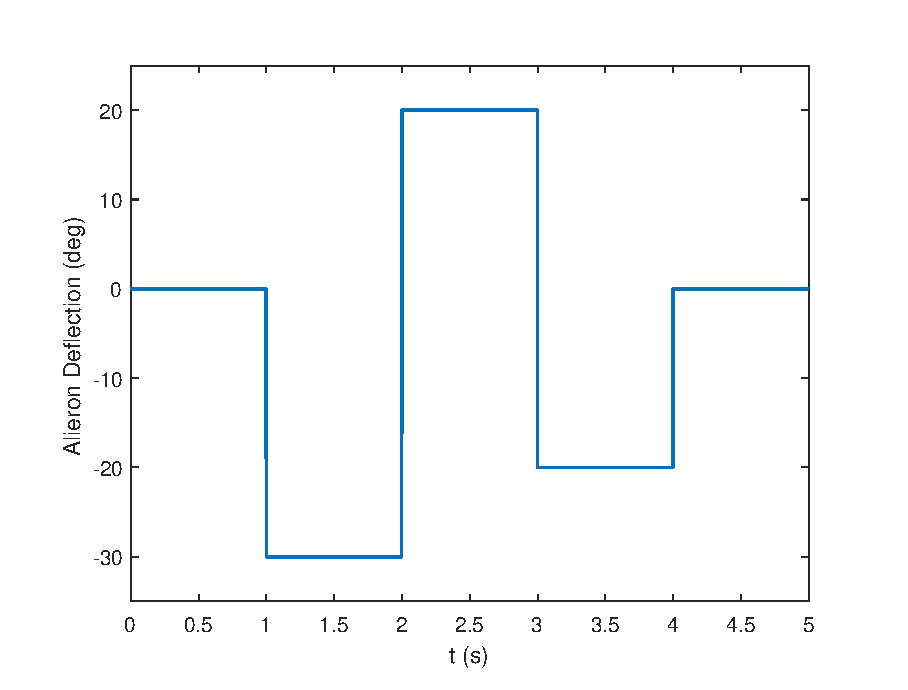
\includegraphics[width=\textwidth]{Imagens/AC_input.eps}
	\caption[entrada]{Simulated elevator command $\delta_a$ as a function of time, in degrees}
	\label{fig:AC_input}
\end{figure}

\begin{figure}[!htb]
	\centering
	\includegraphics[width=\textwidth]{Imagens/AC_noise-realization.eps}
	\caption[entrada]{One realization of noise $\omega$ over time}
	\label{fig:noise_realization}
\end{figure}


\begin{figure}[!htb]
	\centering
	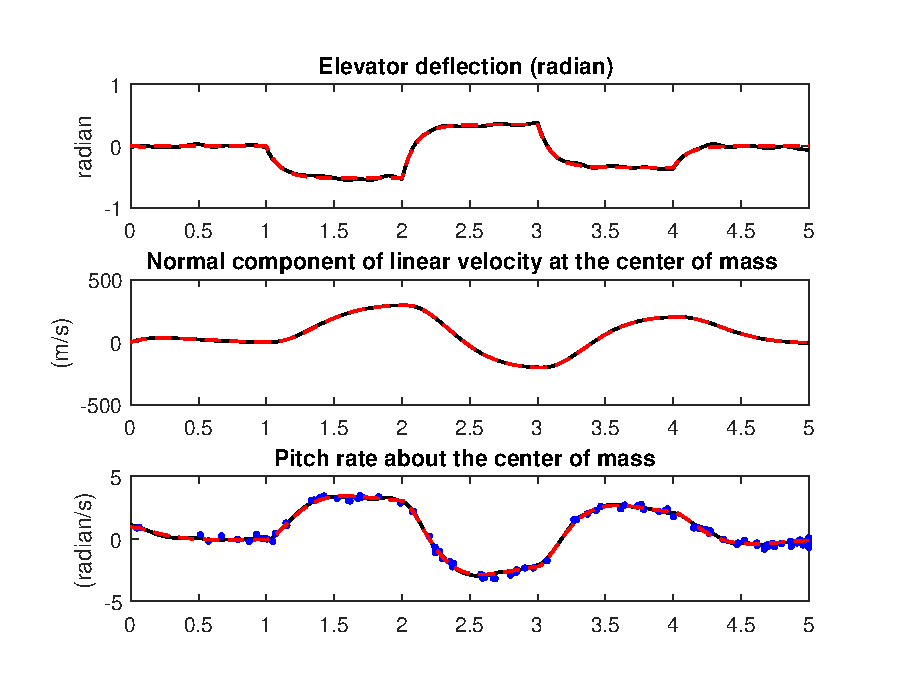
\includegraphics[width=\textwidth]{Imagens/AC_realization.eps}
	\caption[entrada]{The true values (---) and estimated values (\textcolor{red}{- -}) of all three states. For the observed state (pitch rate), the measurements are also shown (\textcolor{blue}{\textbullet})}
	\label{fig:AC_realization}
\end{figure}



\begin{figure}[!htb]
	\centering
	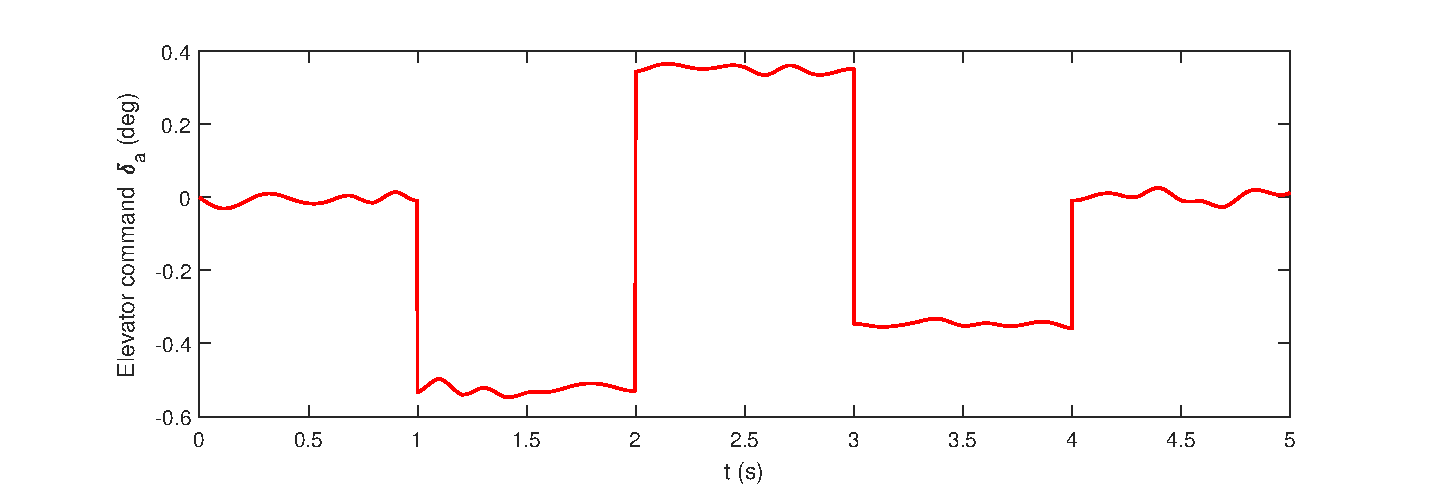
\includegraphics[width=0.75\textwidth]{Imagens/AC_input-noise.eps}
	\caption[entrada]{For a white noise generated at 0.1s timestep and 0.015 variance.}
	\label{fig:AC_input2}
\end{figure}

\begin{figure}[H]
	\centering
	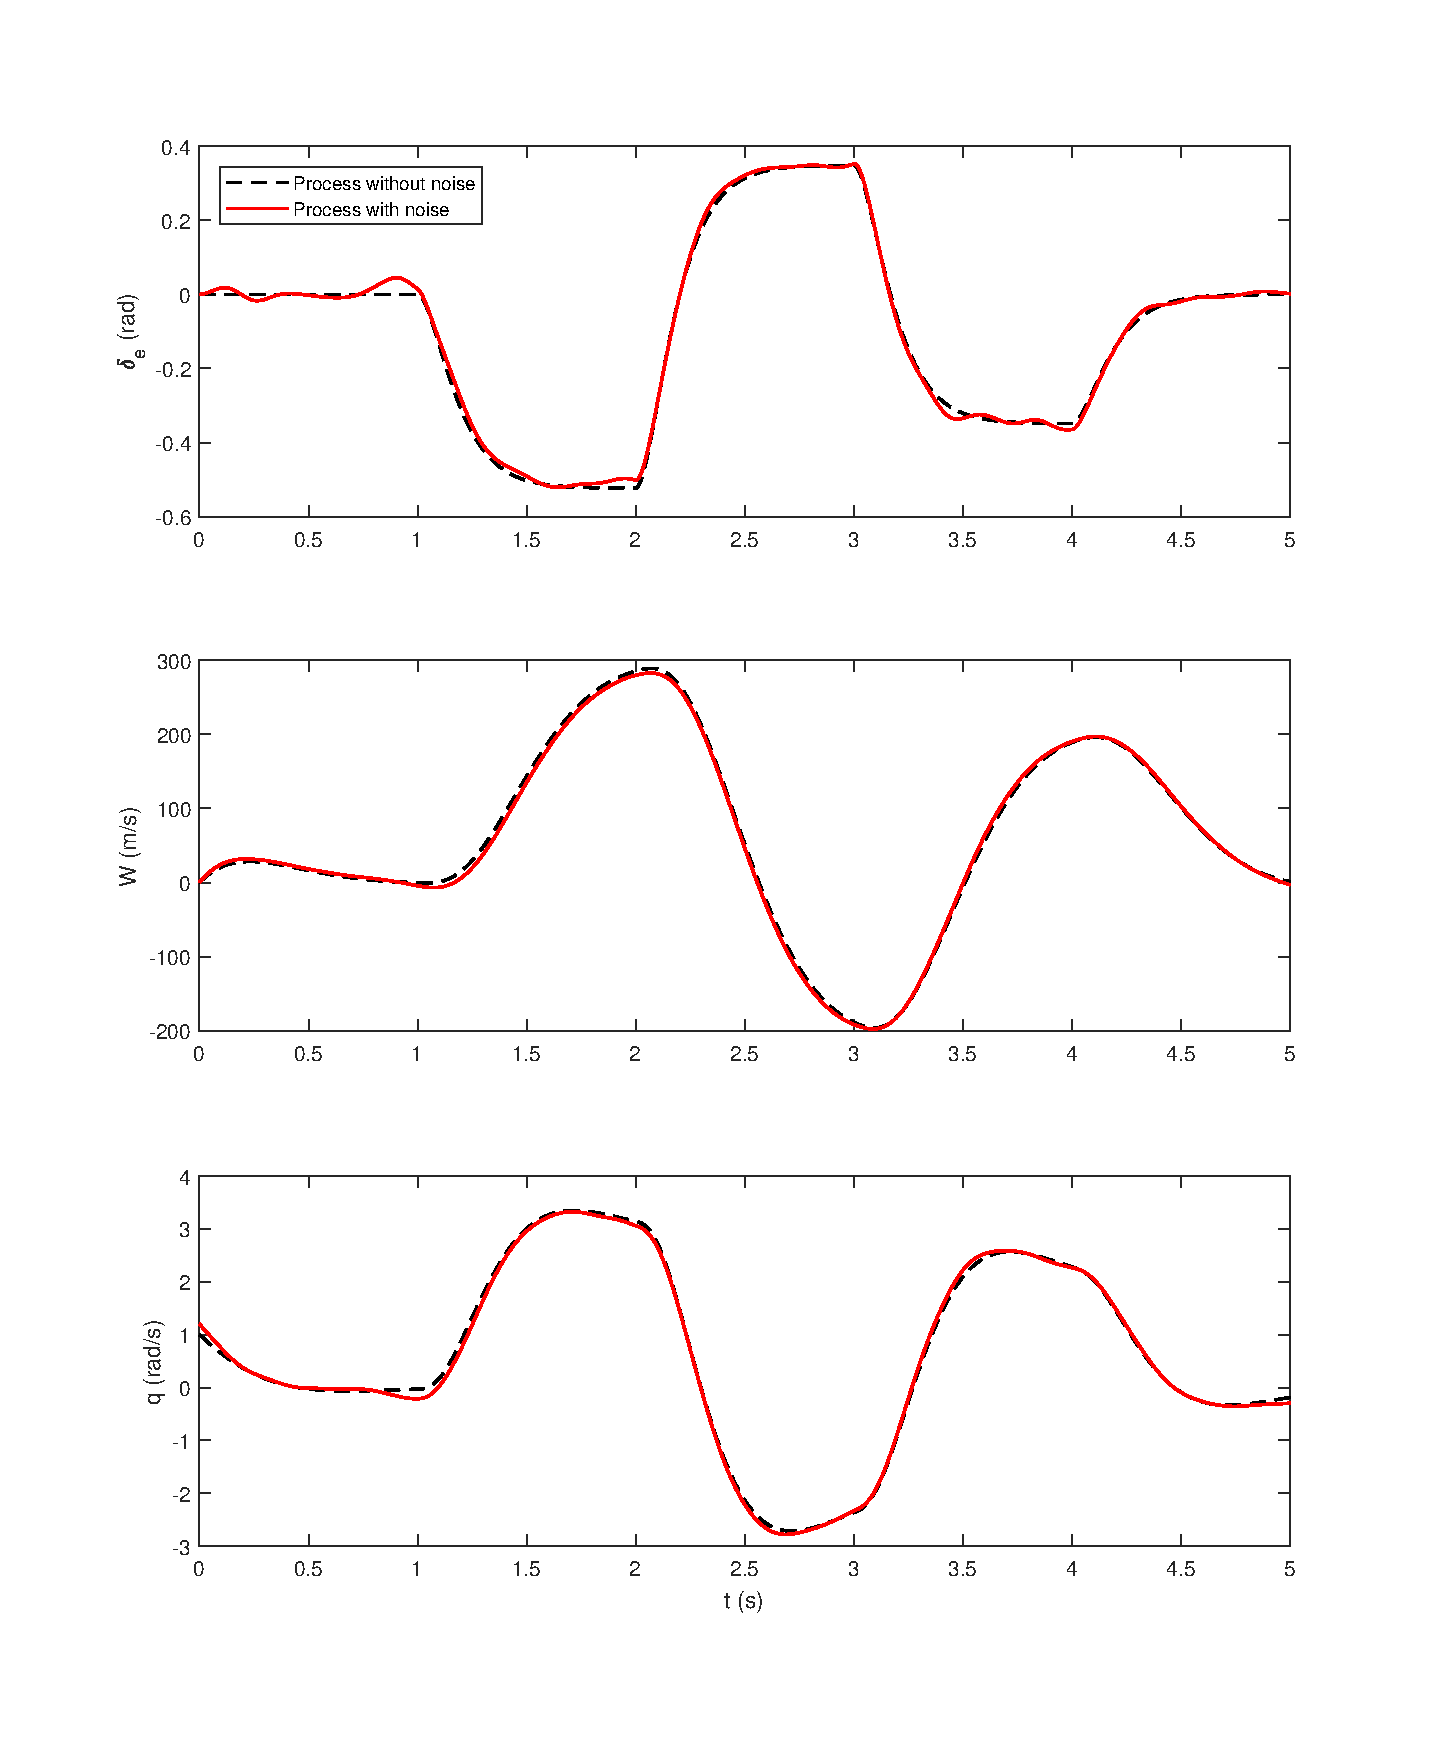
\includegraphics[width=0.75\textwidth]{Imagens/AC_realization2.eps}
	\caption[entrada]{The process simulation without noise (---) and noisy realization (\textcolor{red}{- -}) of all three states. Proce}
	\label{fig:AC_realization2}
\end{figure}


Performance of estimator algorithm is evaluated by the root mean square error (RMSE) of each state, defined by

\begin{equation}\label{eq:ACinddesemp}
RMSE_i = \sqrt{\frac{1}{N}\sum_{k=1}^{N} (x_{\textrm{true},i}[k] -x_{\textrm{est},i}[k])^2 }
\end{equation}

\noindent
where $i$ is the state index, $N$ is the amount of estimates, $x_{\textrm{true},i}$ the true value of the state $i$ sampled at regular time intervals $T$ and $x_{\textrm{est},i}$ the algorithm estimates at the same time instants.

Figure~\ref{fig:AC_J} presents a window data from 0 to 0.2 seconds of the pitch rate about the center of mass RMSE for the algorithms with and without time-stamp, considering XXXXXXXXXX. Again, as expected, we observe a distancing from the RMSE at the instant the first observation was taken $t_1$, favoring the algorithm that considers time-stamp. The reduction in RMSE is lower for the algorithm that assimilates the observed data at the wrong time instant. At $t_2$ the reduction in RMSE happens at the correct time for the algorithm with time-stamp and at the next regular estimation instant for the algorithm that does not consider the time in which observation was taken.

\begin{figure}[H]
	\centering
	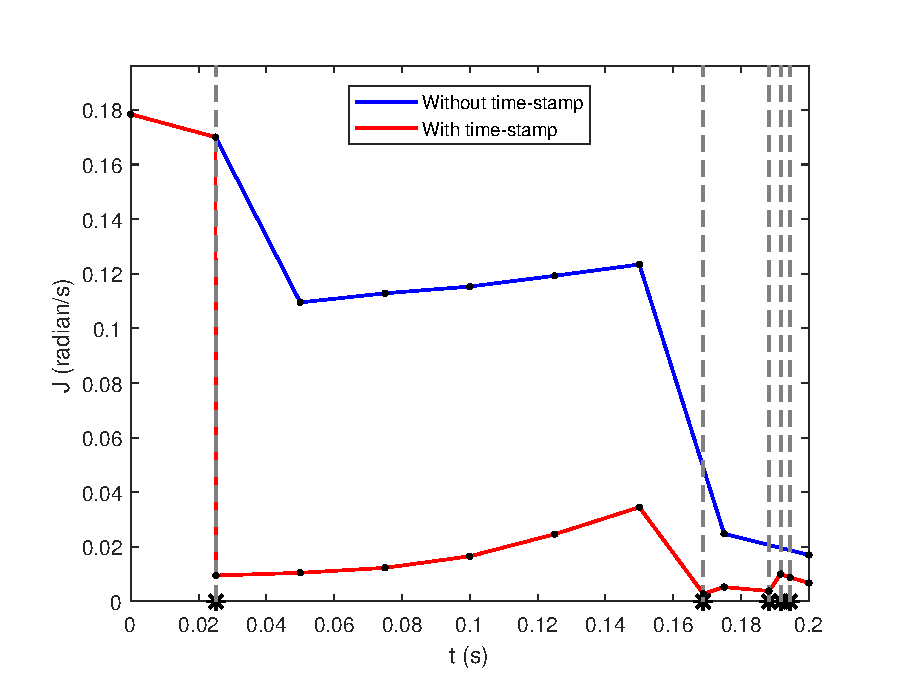
\includegraphics[width=0.8\textwidth]{Imagens/AC_J_evolution.eps}
	\caption[entrada]{Temporal cut from 0 to 0.2 seconds, for a realization of pitch rate about the center of mass RMSE of both estimators, with (\textcolor{red}{---}) and without (\textcolor{blue}{---}) time-stamp. Vertical dashed lines match the measurement sampling instants $t_k$. Black dots represent the regular estimation instants.}
	\label{fig:AC_J}
\end{figure}



\subsection{Measurement Signal-to-Noise Ratio Variation}\label{sec:ruido-AC}

For the aircraft case study, we compare algorithm performance for the same observation signal-to-noise ratio values as for the robot, SNR\textsubscript{y} = $\infty$,  $80$, $60$, $40$, $20$ an $10$ dB. The sampling rate parameters are held constant, $\lambda = 0.1$ s and $\alpha = $ 1s.

We simulate 300 realizations for each scenario and each algorithm. The results for all three system states are shown in Figure~\ref{fig:AC_noise}. Solid lines represent the average values for RMSE and the dashed lines are the 95\% confidence interval.

\todo[inline]{Falta incluir resultados com time-delay}


\begin{figure}[H]
	\centering
	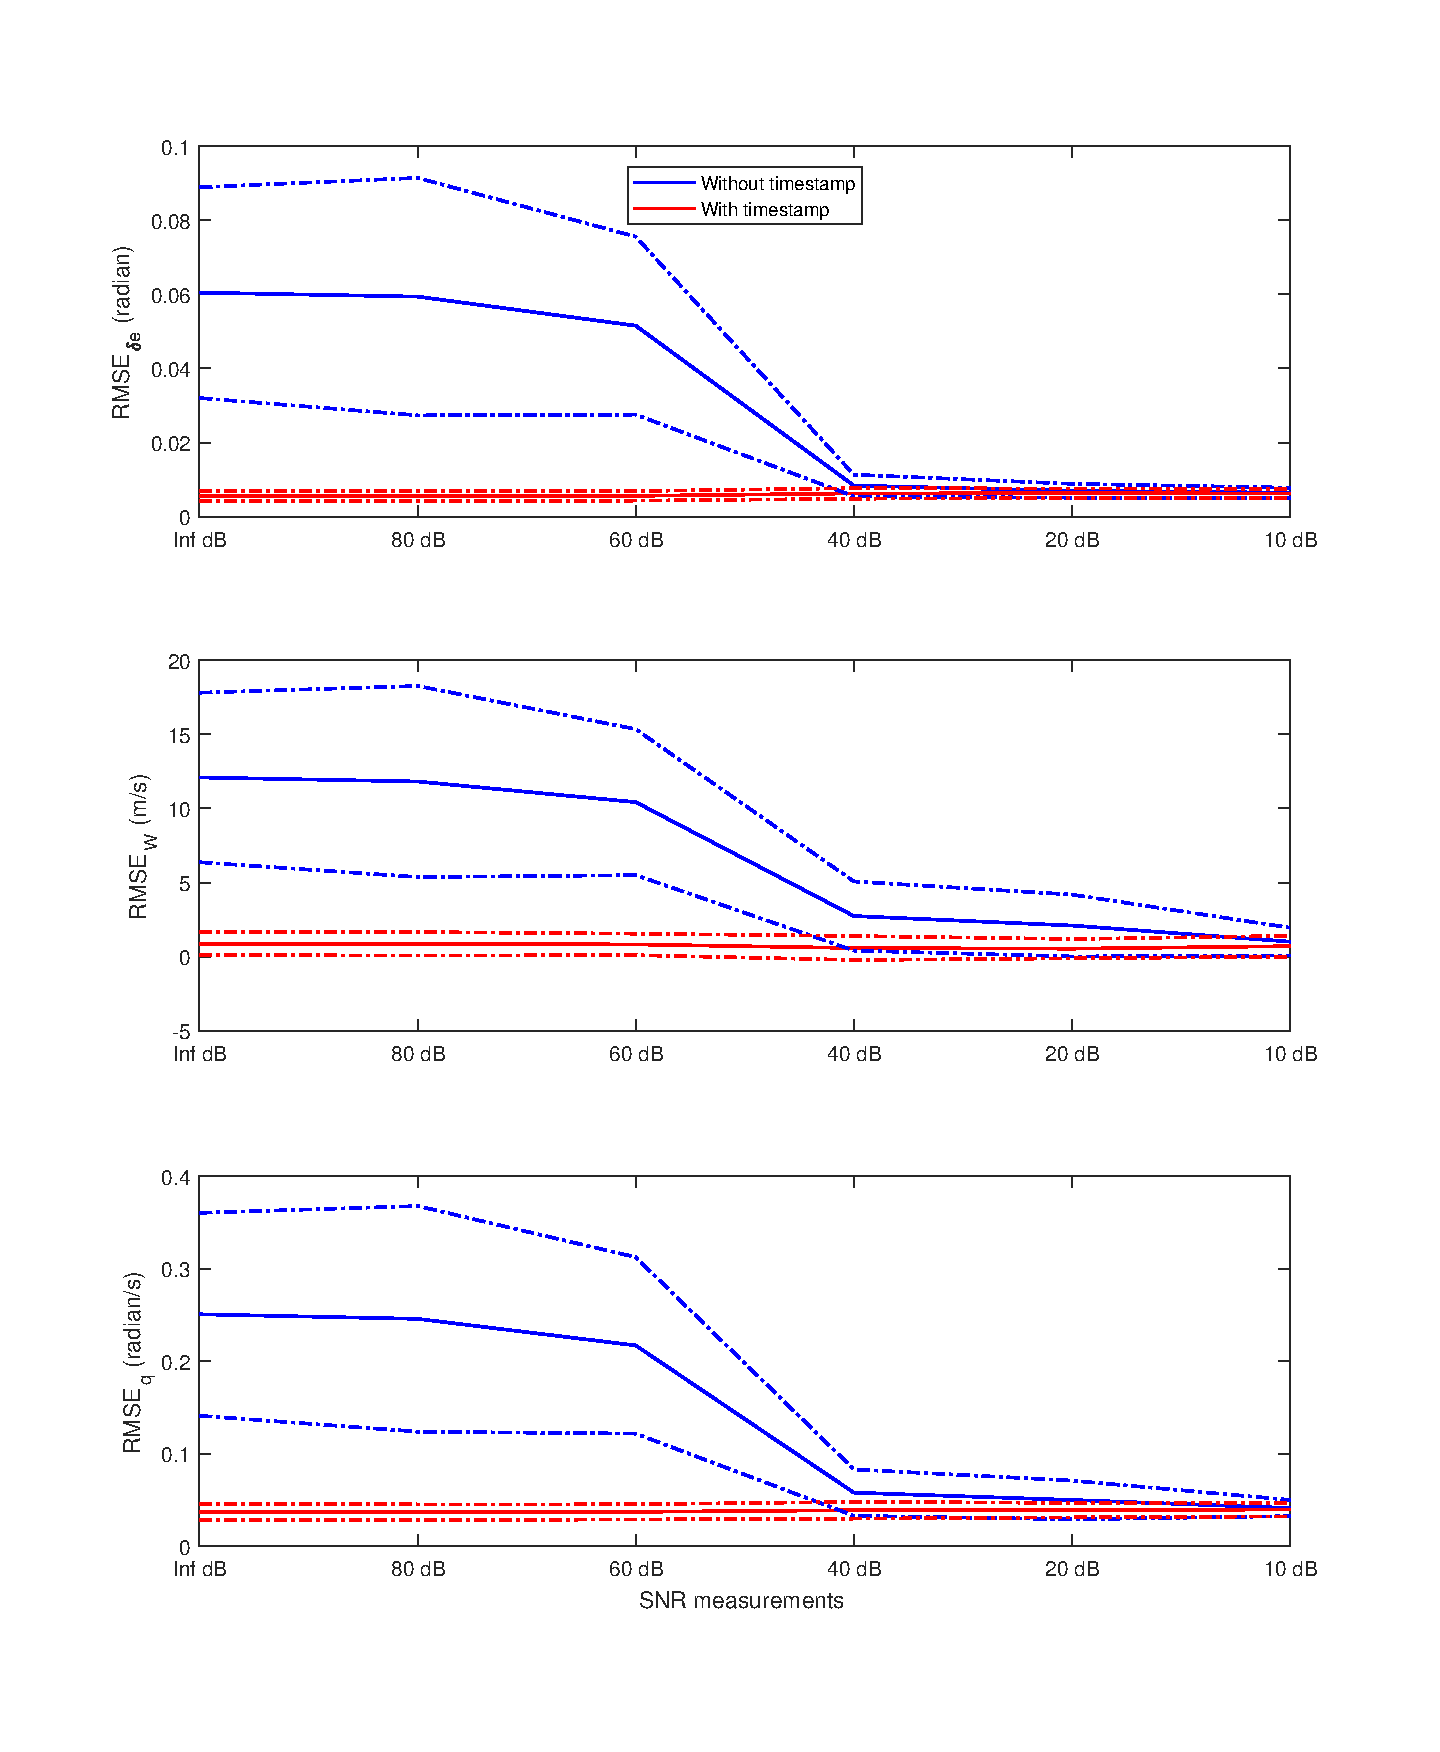
\includegraphics[width=0.8\textwidth]{Imagens/AC_noise.eps}
	\caption[entrada]{Root mean square error variation, as a function of measurement noise for both SDKF algorithms, considering and not considering time-stamp}
	\label{fig:AC_noise}
\end{figure} 

\begin{figure}[H]
	\centering
	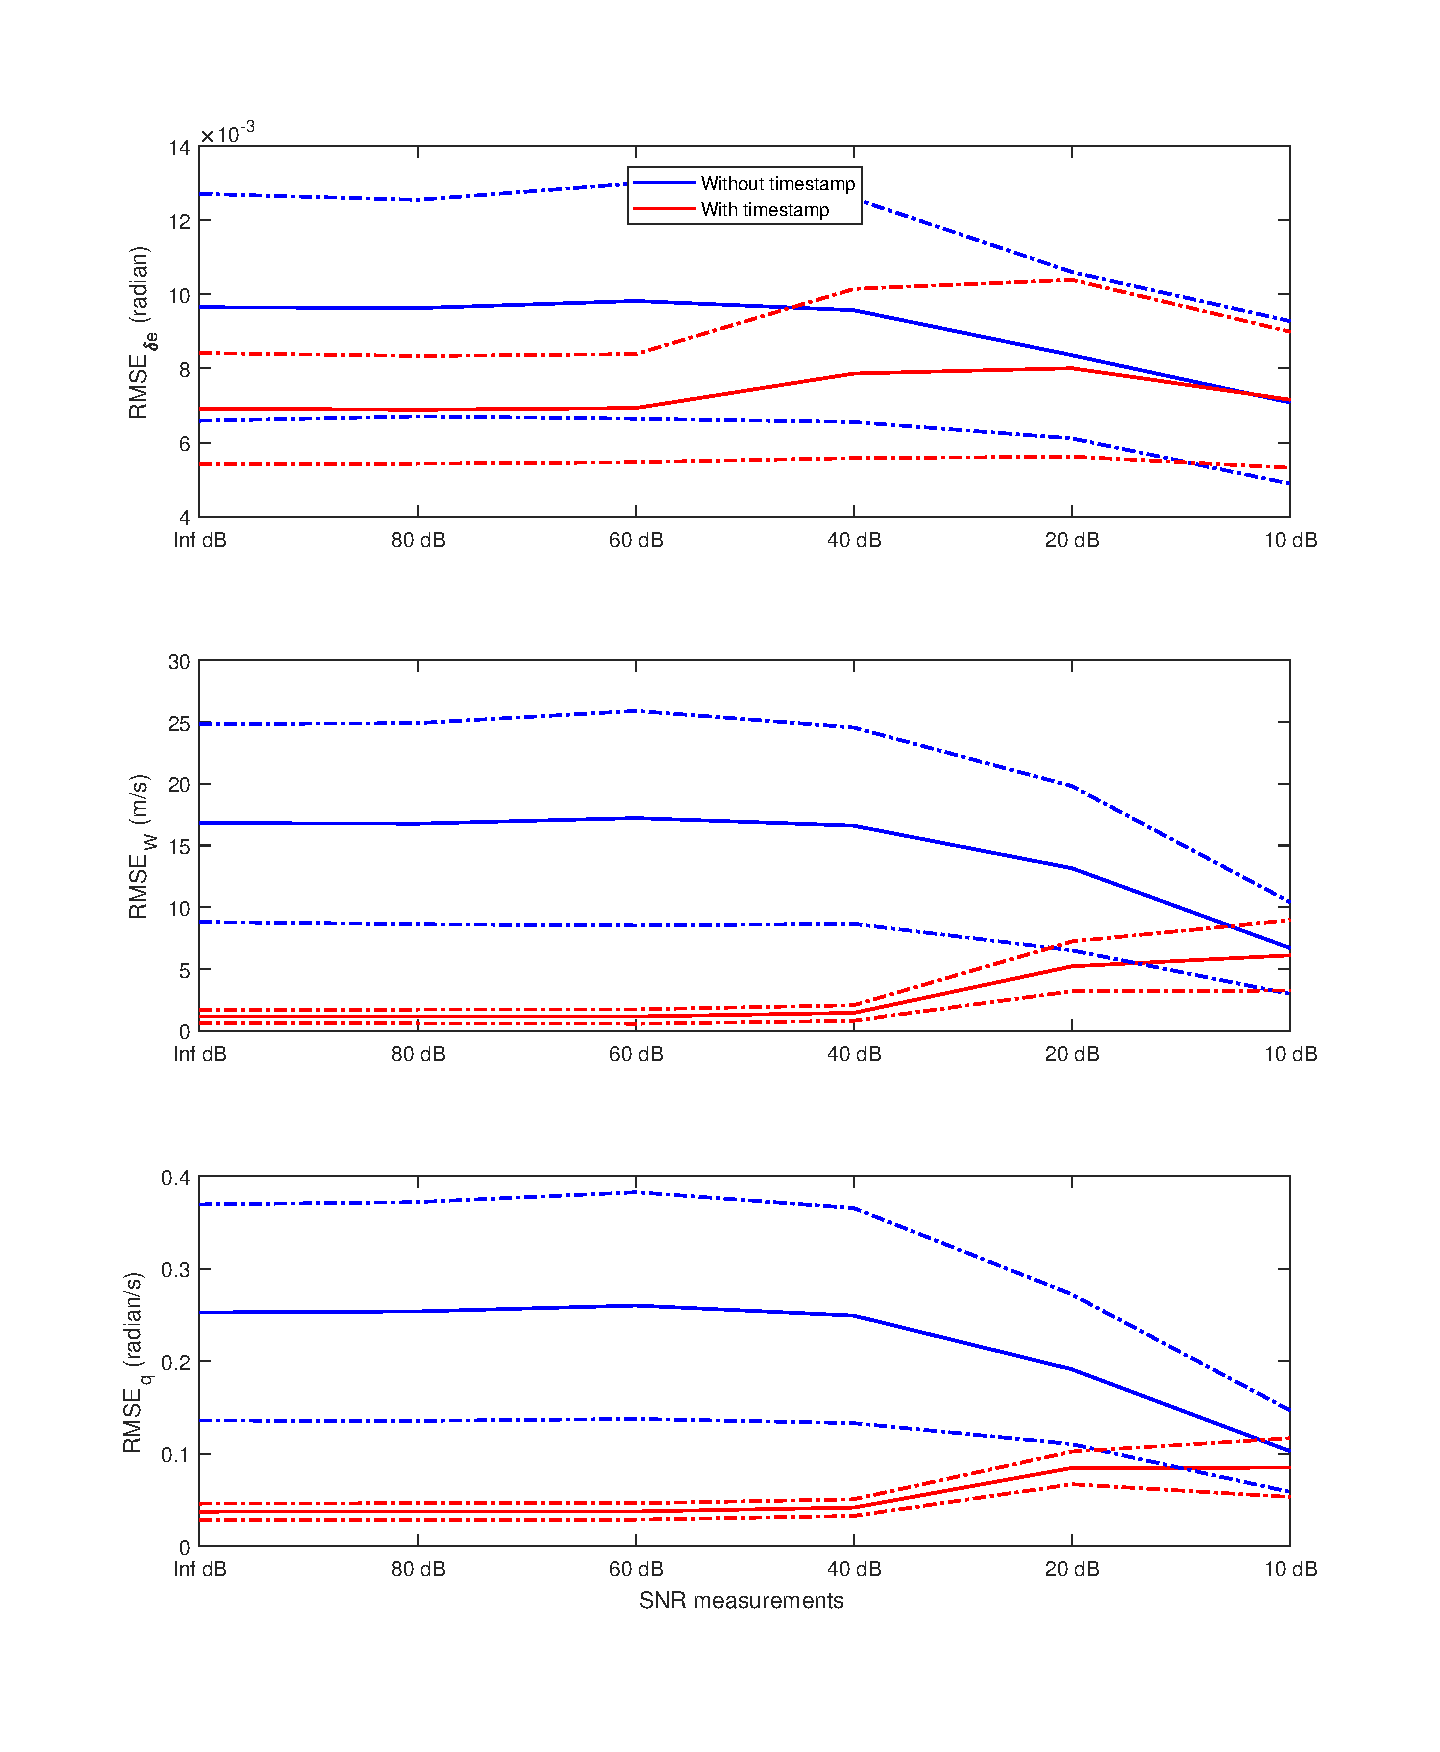
\includegraphics[width=0.8\textwidth]{Imagens/AC_noise-DKF.eps}
	\caption[entrada]{DISCRETE KALMAN FILTER. Root mean square error variation, as a function of measurement noise for both KF algorithms, considering and not considering time-stamp}
	\label{fig:AC_noise-DKF}
\end{figure} 


\textit{Falta resultados com time-delay, para uma an�lise abrangente das figuras}


\subsection{Average Sampling Rate Variation}\label{sec:lambda-AC}

Variation of the observation average time interval for the aircraft was chosen according to $\lambda =$ $0.01$, $0.05$, $0.1$, $0.2$ and $0.5$. We kept noise level and the ratio between estimation and measurement sampling time interval, respectively at SNR\textsubscript{y} $= 60$ and $\alpha = 1$. After 300 realizations for all parameter scenarios and each algorithm, the RMSE results are shown in Figure~\ref{fig:AC_samp}. As usual, the solid lines are the average values of RMSE and the dashed lines comprehend the 95\% confidence interval.

\begin{figure}[H]
	\centering
	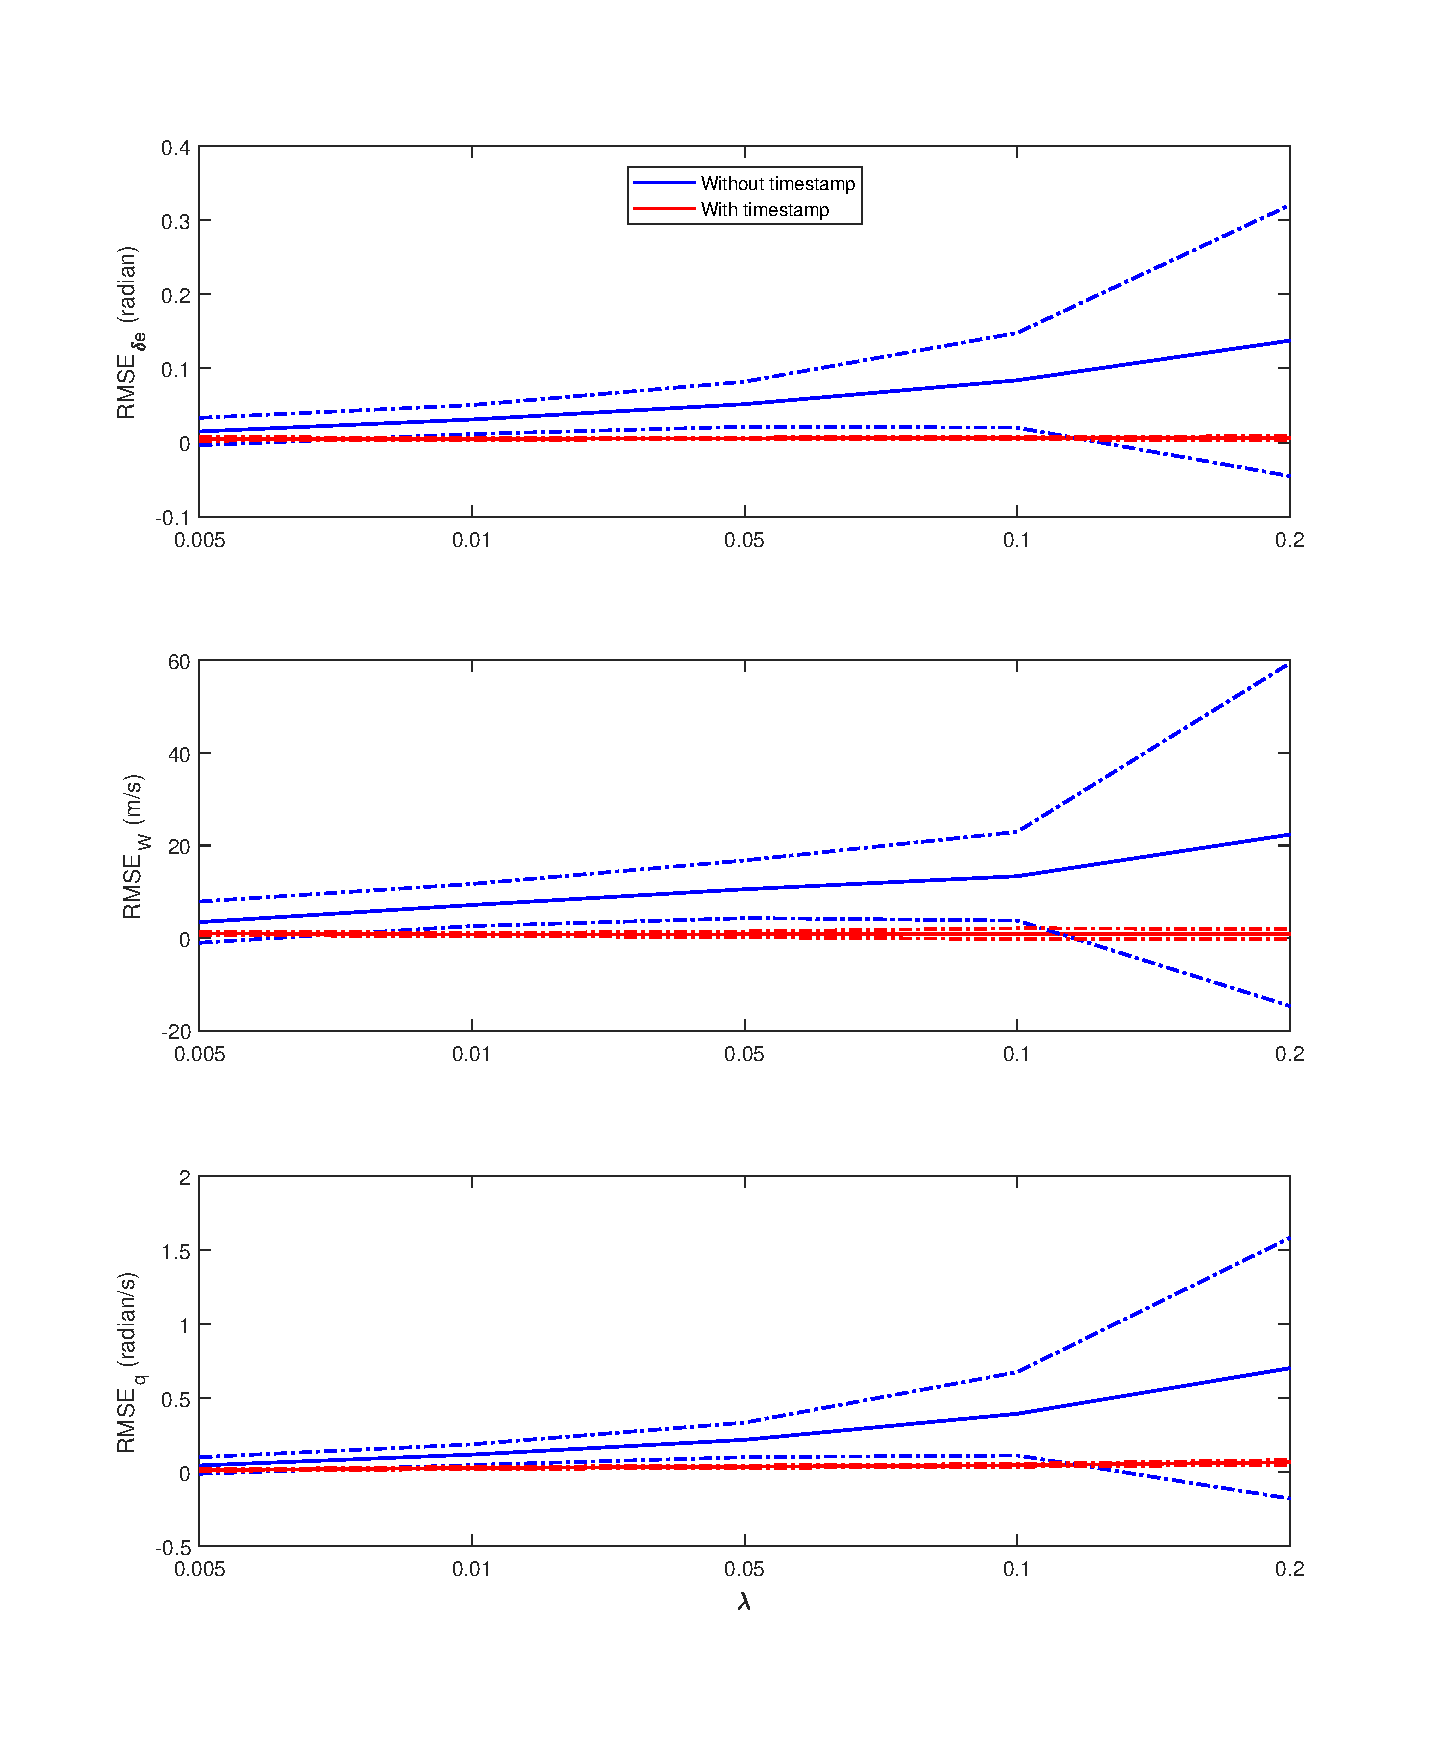
\includegraphics[width=0.8\textwidth]{Imagens/AC_samp-snr60-a1.eps}
	\caption[entrada]{Root mean square error variation, as a function of measurement noise both SDKF algorithms considering and not considering time-stamp}
	\label{fig:AC_samp}
\end{figure}


\textit{Falta resultados com time-delay, para uma an�lise abrangente das figuras}


\subsection{Regular and Average Irregular Time Interval Relation Variation}\label{sec:alpha-AC}

We also simulate the same values used for the robot case study, for regular and irregular time interval ratio, $\alpha = 10$, $5$, $2$, $1$. Measurement noise was kept at SNR\textsubscript{y} $= 40$, and average time interval for observation at $\lambda = 0.1$ s.

The average variation of RMSE and the 95\% confidence interval for 300 realizations are shown in Figure~\ref{fig:AC_dtudty}.

\begin{figure}[H]
	\centering
	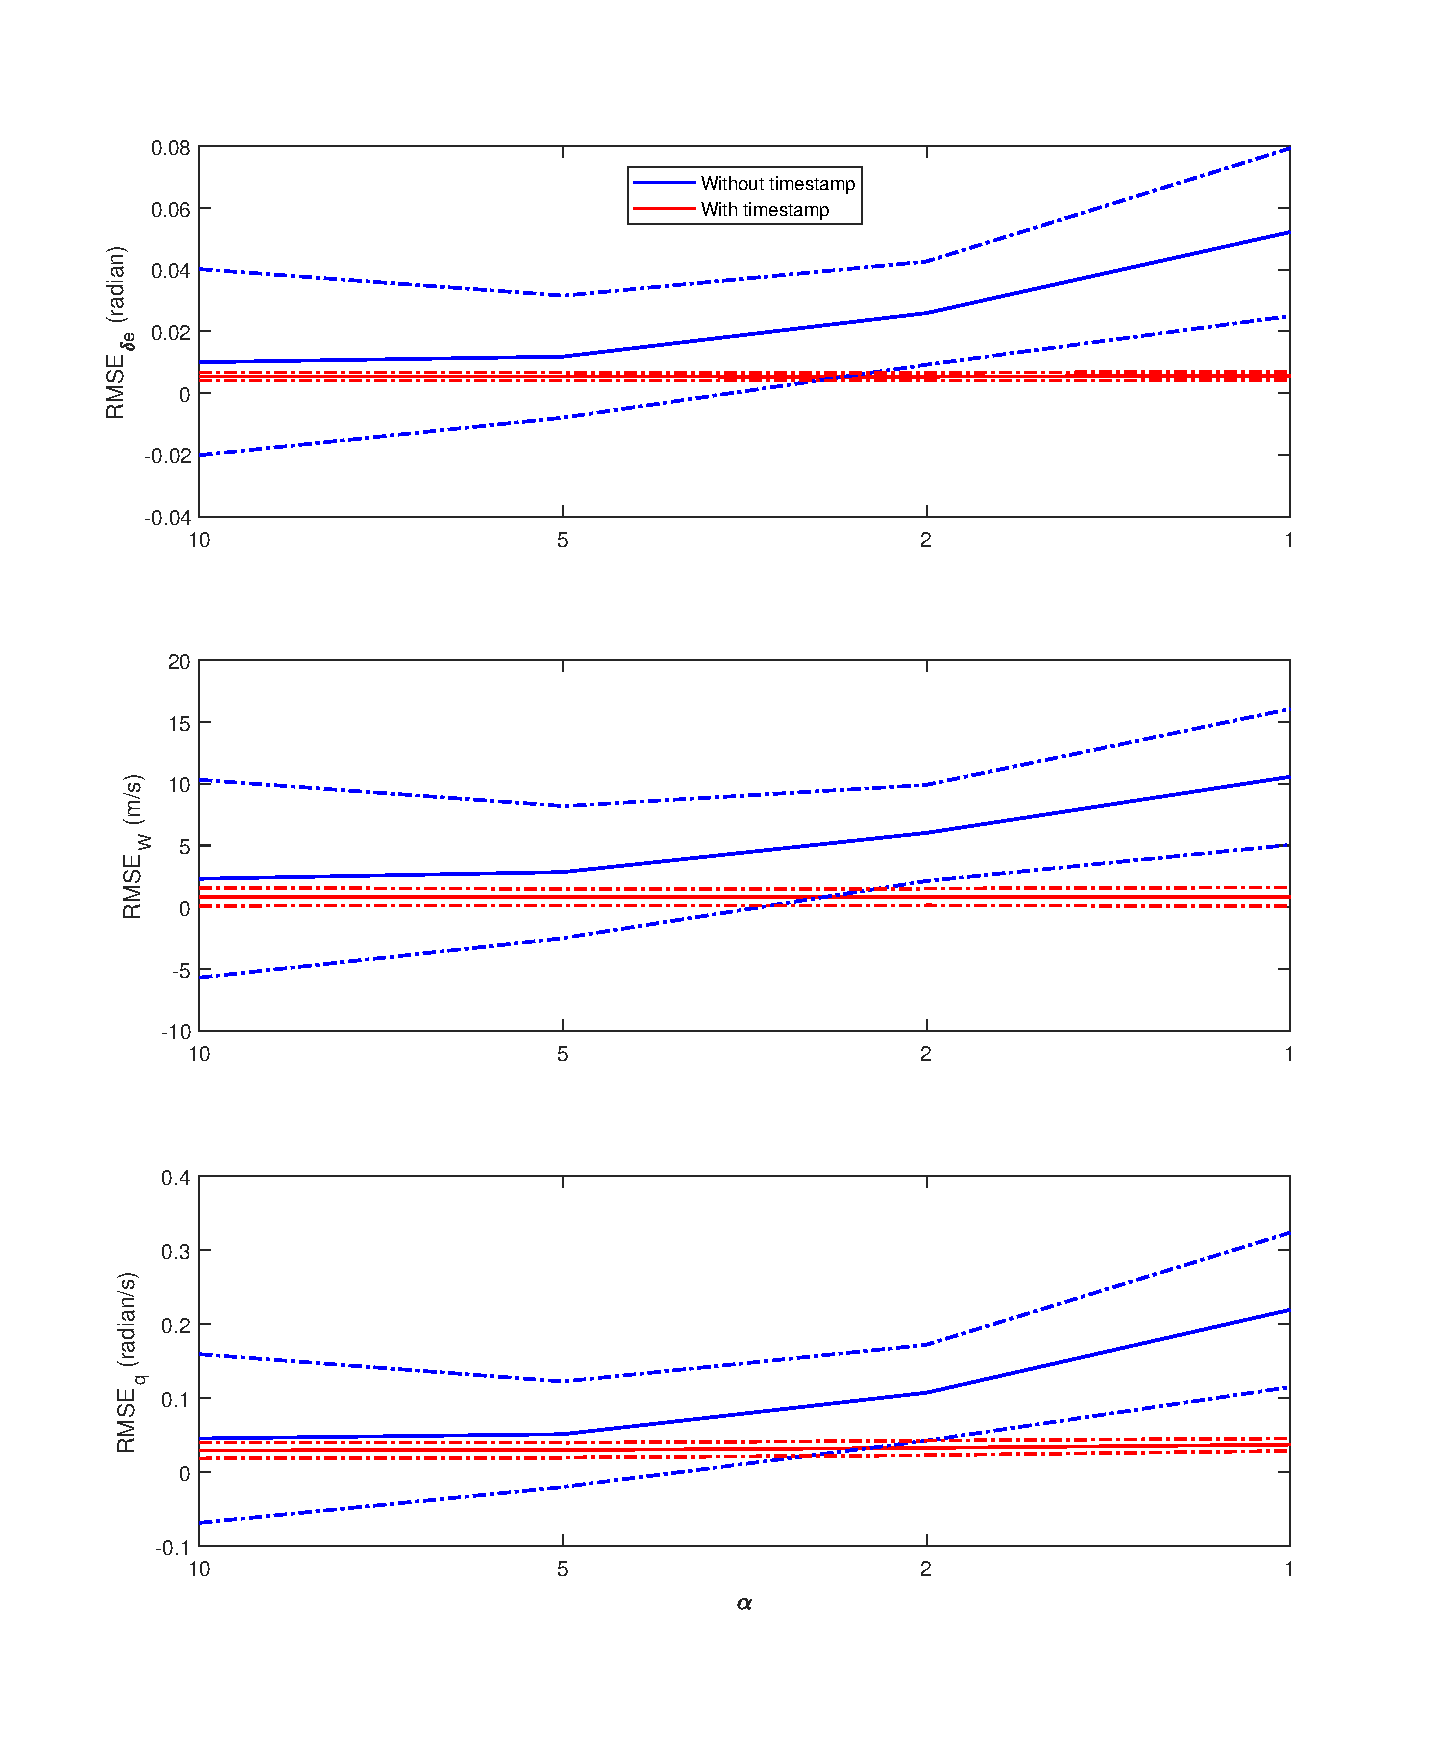
\includegraphics[width=0.8\textwidth]{Imagens/AC_usamp-snr60-dt1.eps}
	\caption[entrada]{Root mean square error variation, as a function of measurement noise both SDKF algorithms considering and not considering time-stamp}
	\label{fig:AC_dtudty}
\end{figure}


\textit{
	Nota-se que, quando o carimbo de tempo � considerado, n�o h� diferen�a significativa em se variar o $\alpha$ no desempenho do filtro, com o �ndice de desempenho $J$ se mantendo pouco abaixo dos $3$ cm. Ou seja, n�o importa a rela��o entre as frequ�ncias de amostragem da observa��o e das entradas. Por outro lado, quando n�o se considera o carimbo de tempo, essa rela��o se torna relevante para o �ndice de desempenho do estimador. Quanto mais lento a frequ�ncia da entrada em compara��o com a frequ�ncia da sa�da, maior o erro obtido. Para o caso mais extremo utilizado, $\alpha=1$, a diferen�a no �ndice $J$ foi mais do que o dobro. Esse resultado era esperado, uma vez que quanto maior o valor de $\alpha$, mais r�pida � a taxa de discretiza��o do modelo de processo em rela��o � frequ�ncia dos sensores de observa��o. Consequentemente, o erro obtido na aproxima��o $\tilde{y}(i) \approx y(t_k)$ diminui.
}

\subsection{Average Time Delay}\label{sec:dt-AC}

\todo[inline,caption={Falta variar o atraso nas medi��es}]{Ainda ter� uma se��o com a varia��o do time-delay e seu impacto no desempenho}


\section{Unicycle Position Estimation}

\textit{Descrever as motiva��es por tr�s do estudo da amostragem irregular para problemas de rastreamento de rob�s. Exemplos: medi��es feitas por c�meras n�o sincronizadas e utilizando redes de internet (com time delay).}

\subsection{System Description}

Consider a nonholomonic moving robot, with the cinematic process model given by

\setlength{\abovedisplayskip}{0.5pt}

\begin{equation}\label{eq:sistema}
\begin{split}
\dot{p}_\textrm{x} & = v\cos (\theta),\\
\dot{p}_\textrm{y} & = v\sin (\theta),\\
\dot{\theta}  & = u_1(t),\\
\dot{v} & = u_2(t),
\end{split}
\end{equation}

\noindent
where $p_\textrm{x}$ and $p_\textrm{y}$ are the position coordinates, $\theta$ the angular orientation, $v$ the linear velocity and inputs $u_1$ and $u_2$ are the angular velocity $\omega$ and the linear acceleration $a$, respectively. Figure~\ref{fig:robot} shows a schematic of the robot and its states,

\begin{figure}[!htb]
	\centering
	\includegraphics[width=0.4\textwidth]{Imagens/Nonholomonic-robot.pdf}
	\caption[entrada]{Nonholomonic robot system representation. The system states $p_\textrm{x}$, $p_\textrm{y}$, $v$ and $\theta$ are highlighted.}
	\label{fig:robot}
\end{figure} 

The system described by~\ref{eq:sistema} is discretized by a 4$^{th}$ order Runge-Kutta method and the state vector $x_i$ is given by $x_i \overset{\Delta}{=} [p_{\textrm{x},i}\ p_{\textrm{y},i}\ \theta_i\ v_i]^T$.

The observation model $y(t_k) \in \mathbb{R}^2$

\begin{equation}
y(t_k) = 
\begin{bmatrix}
p_\textrm{x}(t_k) \\
p_\textrm{y}(t_k)
\end{bmatrix}+v(t_k), \\
\end{equation}

\noindent
is given by the position coordinates and $v(t_k) \sim \mathcal{N} (0,R_{t_k})$ is the observation noise, with zero mean and covariance $R_{t_k}$. When time-stamp is not available, the observation vector is approximated by $\tilde{y}_i \approx y(t_k)$, where $i$ is the index of the next time instant, multiple of $T$.

Input vector $u_i = [\omega_i\ a_i]^T$ is measured by a girometer and accelerometer, respectively. We assume that 

\begin{equation}\label{eq:entrada}
u_i = \tilde{u}_i - w_i,
\end{equation}

\noindent
where $\tilde{u}$ is the sensors measured valueand $w \sim \mathcal{N} (0, Q_i)$ represents the corresponded noise, of zero mean and covariance $Q_i$. 

We simulate 60 seconds of robot movement, considering a step size of $\delta t_{\textrm{sim}} = 10^{-4}$. Irregular sampling time intervals $h_k$ are simulated by the exponential probability distribution function from MatLab\texttrademark \ and approximated to the nearest discrete time instant, from the 600,000 available samples. Input signals were generated arbitrarily according to Figure~\ref{fig:entrada}. Figure~\ref{fig:exukf} shows robot trajectory on $xy$-plane for the given input signals, leaving from point $(0,0)$, as well as a realization of noisy and aperiodic measurements with signal-to-noise ratio of SNR\textsubscript{y} $= 30$ dB and $\lambda=0.3$ s as red dots and the hatched blue line represents UKF estimation, considering time-stamp, $\alpha=5$ and SNR\textsubscript{u} $= 10$ dB. 


\begin{figure}[!htb]
	\centering
	\begin{subfigure}
		\centering
		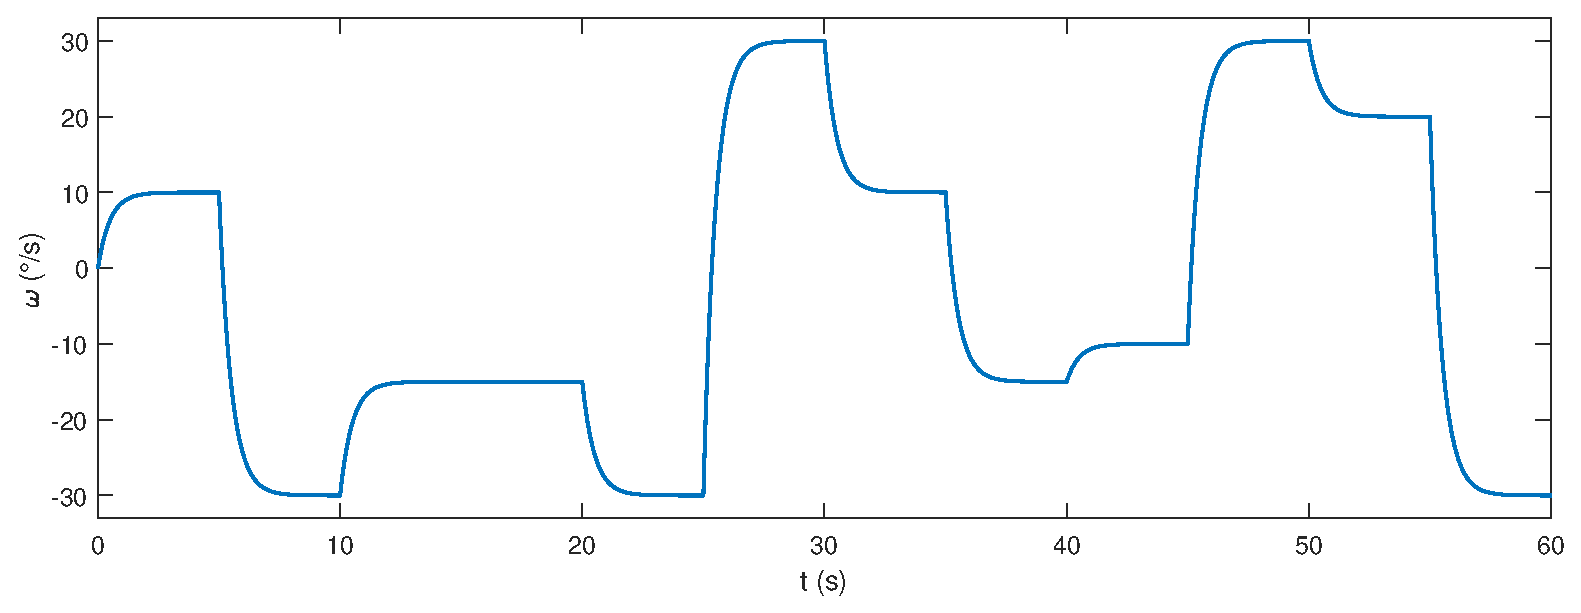
\includegraphics[width=\textwidth]{Imagens/entradas1.eps}	
		%		\caption{}
		\label{fig:sfig1}
	\end{subfigure}
	\begin{subfigure}
		\centering
		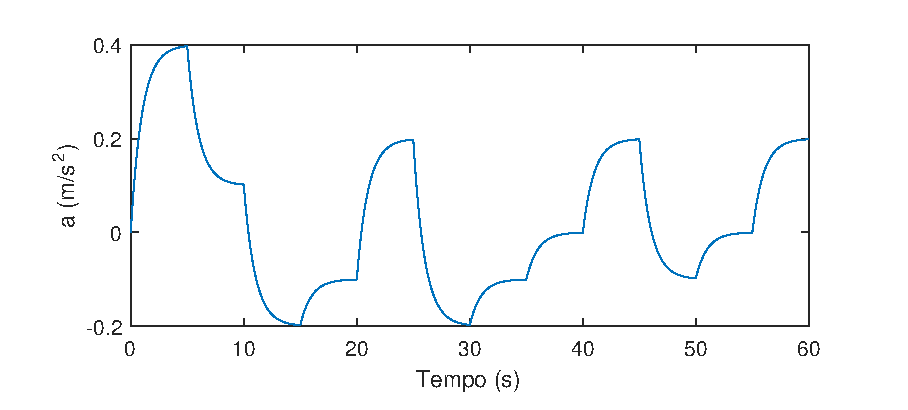
\includegraphics[width=\textwidth]{Imagens/entradas2.eps}
		%		\caption{}
		\label{fig:sfig2}
	\end{subfigure}
	\caption[Entradas]{Simulation input signals. (a) shows temporal sequence of angular velocity $\omega$ and (b) shows linear acceleration $a$.}
	\label{fig:entrada}
\end{figure}

\begin{figure}[!htb]
	\centering
	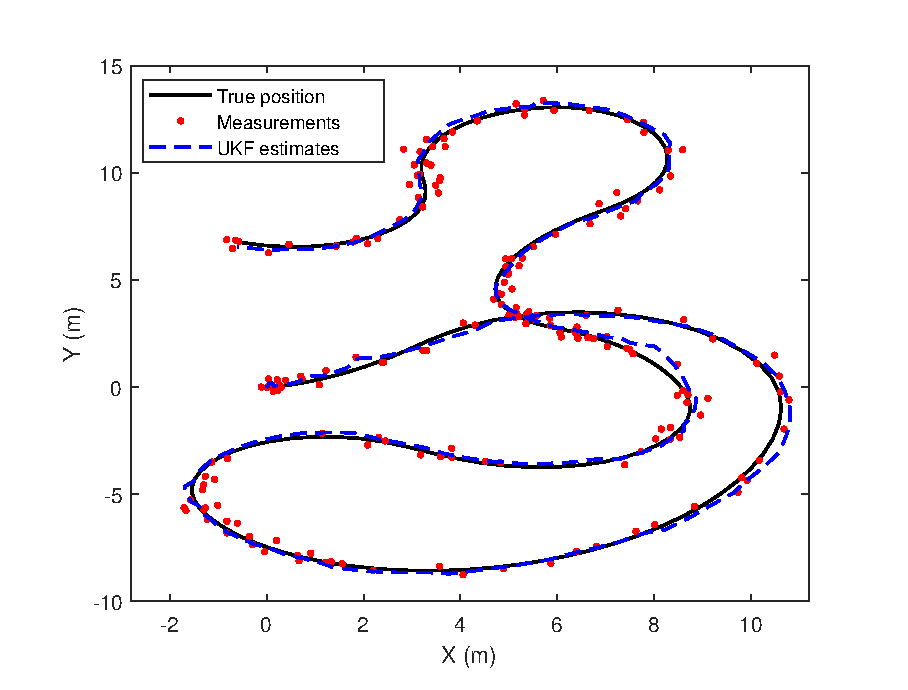
\includegraphics[width=0.8\textwidth]{Imagens/exemplo_03_30db_desloc.eps}
	\caption[entrada]{True position, noisy measurements and UKF estimates considering time-stamp, for a measurement noise of SNR\textsubscript{y} $= 30$ dB, $\lambda=0.3$ s and $\alpha=5$.}
	\label{fig:exukf}
\end{figure} 

To analyze the effect of considering time-stamp in the estimation algorithm, we use the performance index $J$

\begin{equation}\label{eq:inddesemp}
J = \frac{ \sum_{i=1}^N \sqrt{(\hat{p}_{\textrm{x},i}-p_{\textrm{x},i})^2+(\hat{p}_{\textrm{y},i}-p_{\textrm{y},i})^2}}{N}
\end{equation}

\noindent
where $\hat{p}_{\textrm{x},i}$ and $\hat{p}_{\textrm{y},i}$ are filter position estimates produced at a regular interval $T$, $\hat{p}_{\textrm{x},i}$ and $\hat{p}_{\textrm{y},i}$ the true coordinates of the robot at the same time instants and $N$ the total number of estimates. This index represents the average estimator position error in $xy$-plane.

Figure~\ref{fig:realizacaoJ} shows a timespan from 0 to 1.3 seconds of a $J$ realization, considering $\lambda=0.5$, $\alpha=5$, SNR\textsubscript{y} $=60dB$ dB and SNR\textsubscript{u} $=20$ dB, for the UKF considering and not considering time-stamp. Black dots represent the regular time instants $kT$ whereas the asterisks on x-axis match the exact measurement instants $t_k$. As expected, before the first data assimilation steps, both performances are identical. Since the first measurement $t_1$ was taken almost at the same time as regular estimation time instant $4T$, both estimation performances maintain close to each other. That is because the approximation error due to $\tilde{y}_i \approx y(t_k)$ is irrelevant. At $t_2$ we can observe significant deviation from index $J$ in benefit of the algorithm considering time-stamp, since it performs data assimilation at the exact time measurement was taken. The same effect can be noted at $t_4$, after 1 second of simulation, when there is a significant different between time the measurement was taken and the next regular estimation instant.


\begin{figure}[!htb]
	\centering
	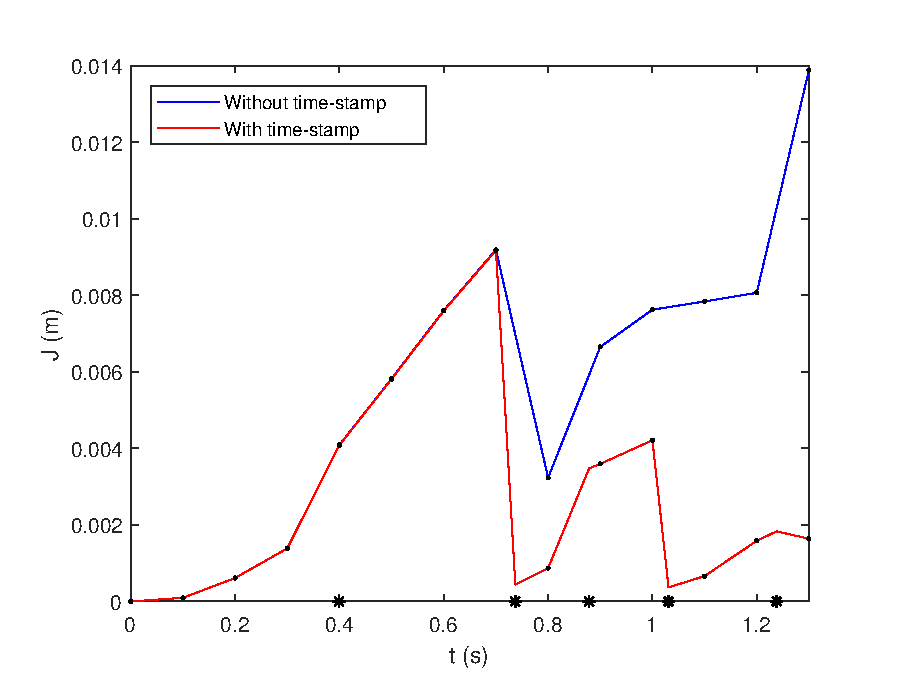
\includegraphics[width=0.8\textwidth]{Imagens/J_umarealizacao.eps}
	\caption[entrada]{Temporal cut from 0 to 1.3 seconds, for a realization of $J$ of both estimators, with and without time-stamp. Asterisks on $x$ axis match the measurement sampling instants $t_k$. Black dots represent the regular estimation instants, same as input regular sampling instants.}
	\label{fig:realizacaoJ}
\end{figure} 

%\begin{figure}[!htb]
%	\centering
%	\includegraphics[width=0.8\textwidth]{Imagens/J_umarealizacao-timedelay.eps}
%%%	\caption[entrada]{Recorte temporal de 1 a 1.3 segundo, do �ndice J de uma realiza��o dos dois estimadores, com e sem carimbo de tempo. Os asteriscos no eixo $x$ representam os instantes de amostragem das observa��es $t_k$. Os pontos pretos apresentados nas linhas representam os instantes de tempo regulares de amostragem da entrada}
%	\label{fig:realizacaoJ2}
%\end{figure} 



%\setlength{\abovedisplayskip}{0.5pt}
%
%\begin{equation}\label{eq:sistema}
%\begin{split}
%\dot{\delta_e} & = -\tau^{-1},\\
%\dot{W} & = Z_{de}\delta_e + Z_wW + S_0q,\\
%\dot{q}  & = S_1 \delta_e + S_2 W + S_3q,\\
%\end{split}
%\end{equation}
%\noindent

\subsection{Measurement Signal-to-Noise Ratio Variation}\label{sec:ruido-robo}

In this subsection we compare the estimation performance impact of considering time-stamp in the algorithm, by varying the measurement noise level. The signal-to-noise ratio for the input sensors and the measurement average time interval are held constant, SNR\textsubscript{u} $= 20$ dB and $\lambda = 0.1$ s.

We considered an observation signal-to-noise variation of SNR\textsubscript{y} = $\infty$,  $80$, $60$, $40$, $20$, $10$ dB. That is, initially the system was simulated considering no measurement noise and then it was gradually increased. For each noise scenario, we ran 100 realizations of the random variables for each algorithm and Figure~\ref{fig:noise} shows the results. Solid lines represent the average values for $J$ and the dashed lines are the 95\% confidence interval.

\todo[inline]{Falta incluir resultados com time-delay}


\begin{figure}[!htb]
	\centering
	\includegraphics[width=0.8\textwidth]{Imagens/noise.eps}
	\caption[entrada]{Performance index $J$ variation, as a function of measurement noise for both UKF algorithms considering and not considering time-stamp}
	\label{fig:noise}
\end{figure} 


\textit{� poss�vel observar que o estimador que considera o carimbo de tempo possui desempenho estatisticamente superior apenas para baixos n�veis de ru�do da observa��o. Quando SNR\textsubscript{y} � igual a $\infty$ e $80$ dB, o �ndice de desempenho $J$ do filtro com carimbo de tempo � aproximadamente $1.25$ e $1.26$ cm, respectivamente, mais preciso do que sem carimbo de tempo e com vari�ncia pequena. Quando a rela��o sinal ru�do se aproxima de $40$ dB, no entanto, n�o � poss�vel distinguir estatisticamente o efeito de se considerar ou n�o carimbo de tempo.
}


\subsection{Average Sampling Rate Variation}\label{sec:lambda-robot}

We now consider the variation of the average time interval that observations are taken, according to $\lambda =$ $0.1$, $0.2$, $0.3$, $0.4$, $0.5$, $0.6$ s, maintaining the other parameters constant, namely the noise level of inputs and observations, SNR\textsubscript{u} $= 20$ dB and SNR\textsubscript{y} $= 40$ dB, respectively. We carried out 100 realizations for each $\lambda$ and for each algorithm and Figure~\ref{fig:samp} presents the results. Again, the solid lines are the average values of $J$ and the 95\% confidence interval is between the dashed lines.

\begin{figure}[!htb]
	\centering
	\includegraphics[width=0.8\textwidth]{Imagens/samp.eps}
	\caption[entrada]{Performance index $J$ variation, as a function of measurement noise both UKF algorithms considering and not considering time-stamp}
	\label{fig:samp}
\end{figure}


\textit{Os resultados obtidos demonstram que a diferen�a no desempenho dos filtros � mais significativa para intervalos de tempo mais espa�ados, mantendo-se a din�mica do sistema e os outros par�metros fixos. Inicialmente, para valores pequenos de $\lambda$	, n�o h� diferen�a estat�stica entre o desempenho dos estimadores, mas a medida que o intervalo cresce, ela aparece, chegando a aproximadamente $3.1$ cm para um $\lambda = 0.6$ s. Uma interpreta��o poss�vel � que, se o intervalo de tempo m�dio das observa��es for muito pequeno em compara��o com a velocidade em que a din�mica do sistema varia, o erro de aproxima��o do instante de amostragem das observa��es $t_k$ � reduzido. O ru�do do sensor pode acabar sendo mais relevante do que o erro devido ao tempo incorreto de assimila��o.}


\subsection{Regular and Average Irregular Time Interval Relation Variation}\label{sec:alpha-robot}

We also analyze the performance impact of varying the parameter $\alpha$, which is the relation between regular input time interval $T$ and average measurements time interval $\lambda$. The simulated values were $\alpha = 10$, $5$, $2$, $1$. That means we start with higher frequency values for input sampling in comparison to measurement sampling and this values is gradually decreased. Other parameters were maintained constant SNR\textsubscript{u} $= 20$ dB and SNR\textsubscript{y} $= 40$ dB.

The same way we did for the other scenarios, 100 realizations were simulated and Figure~\ref{fig:dtudty} presents the results. Solid lines are the average values for $J$ and dashed lines represent the 95\% confidence interval.

\begin{figure}[!htb]
	\centering
	\includegraphics[width=0.8\textwidth]{Imagens/dtudty.eps}
	\caption[entrada]{Performance index $J$ variation, as a function of measurement noise both UKF algorithms considering and not considering time-stamp}
	\label{fig:dtudty}
\end{figure}


\textit{
	Nota-se que, quando o carimbo de tempo � considerado, n�o h� diferen�a significativa em se variar o $\alpha$ no desempenho do filtro, com o �ndice de desempenho $J$ se mantendo pouco abaixo dos $3$ cm. Ou seja, n�o importa a rela��o entre as frequ�ncias de amostragem da observa��o e das entradas. Por outro lado, quando n�o se considera o carimbo de tempo, essa rela��o se torna relevante para o �ndice de desempenho do estimador. Quanto mais lento a frequ�ncia da entrada em compara��o com a frequ�ncia da sa�da, maior o erro obtido. Para o caso mais extremo utilizado, $\alpha=1$, a diferen�a no �ndice $J$ foi mais do que o dobro. Esse resultado era esperado, uma vez que quanto maior o valor de $\alpha$, mais r�pida � a taxa de discretiza��o do modelo de processo em rela��o � frequ�ncia dos sensores de observa��o. Consequentemente, o erro obtido na aproxima��o $\tilde{y}(i) \approx y(t_k)$ diminui.
}

\subsection{Average Time Delay}\label{sec:dt-robot}

\todo[inline,caption={Falta variar o atraso nas medi��es}]{Ainda ter� uma se��o com a varia��o do time-delay e seu impacto no desempenho}


\clearpage

\clearpage
\thispagestyle{empty}
\cleardoublepage

%Cap�tulo 5 - Conclusions
%-------------------------------------------------------------------------------
\hypertarget{lcap6}{}
\chapter{Conclusions}
\vspace{-1cm} \label{cap6} 
%\begin{flushright}
%\begin{minipage}{0.7\linewidth}
%\emph{``Enquanto existir vontade de lutar, existem esperan�as de
%vencer.''}
%\end{minipage}
%\end{flushright}
%
%\begin{flushright}
%{A. Agostinho}
%\end{flushright}


\section{Project Overview}

In this study, we investigate how neglecting timestamps of irregularly sampled measurements may affect state estimation performance, under different conditions. 

The research motivations are discussed in Chapters \ref{cap2} and \ref{cap3}, where sensor fusion methods and irregular sampling schemes are reviewed, respectively. We note how sensor fusion, as a field of science, has been experiencing significant growth due to cheaper sensors and communication devices. Bigger and more complex sensor networks are more and more common, and so are the related challenges, such as irregular sampling. Then we define the irregular sampling problem and review the main schemes studied in the literature. Timestamps are often needed in order to take these irregularities into account in data fusion processes. We note that sometimes due to computational complexity or the need of investment in time synchronization techniques, such assumption is not always guaranteed. Thus we conclude the literature review focusing in the study of sensor fusion applied to state estimation and how it is affected when timestamp is neglected.

In Chapter~\ref{cap4} we describe the algorithms used in the numerical simulations. We begin by describing the discrete-time representation of sampled-data systems, considering variable time steps in the discretization process, since measurements are sampled aperiodically. We also review the most popular state estimation algorithm, that is the Kalman Filter (KF), and one of its variation for nonlinear cases, the unscented Kalman Filter (UKF). We describe them as a data fusion process, using the Bayesian framework. Then we describe the sampling irregularity model, which is considered to be given by a Poisson process, meaning that the waiting time between two consecutive measurements is a exponential random variable (RV). Moreover, we describe the adaptations made to the algorithms due to the aperiodic sampled measurements. Whenever timestamps are not available, the measurements are considered to be taken in the next regular estimation interval. A first glimpse of the added error introduced by neglecting timestamps is also presented in this chapter. We end it by defining performance metrics used in the simulation, that cover both accuracy and consistency.

Numerical results are presented in Chapter~\ref{cap5}. We begin by studying the error effects on measurements introduced by shifting the time instants they were taken, and how these errors are related to signal-to-noise ratios (SNR) and system dynamics. Based on that, we propose a simulation setup, where system parameters are varied to assess their relation to state estimation performance, knowingly: (i) measurement noise levels, or SNR; (ii) average sampling rate of measurements, referred to as $\lambda$; and (iii) the relation between $\lambda$ and the regular sampling rate of the estimation, referred to as $\alpha$. Two systems are chosen as case studies: a fourth-order linear time invariant system; and a nonlinear system given by a nonholomonic moving unicycle robot, whose position in the $xy$-plane must be estimated. We illustrate the state estimation problem under irregular sampling by one realization of the estimates. To assess the performance differences from the algorithms that consider and neglect measurement timestamps, we run multiple simulations and calculate the performance metrics mean values and effect sizes in a confidence interval of $95\%$, which are then compared and discussed.

\section{Main Results and Contributions}

We consider the research objectives introduced in the beginning of this work to be achieved. As for the first one, an extensive review in sensor fusion as a field of science is provided, considering its motivations and the taxonomies proposed in literature. We also categorize and discuss most of the irregular sampling models studied by state estimation applications. 

We then choose Kalman filter and the unscented Kalman filter as state estimation methods, presenting their implementation details. By modeling the measurements random time instants as a Poisson process, we cover a very generic irregular sampling problem. The motivations behind it lie on large sensor networks applications, where data is transmitted periodically but unsynchronized. Resulting arrival times can be approximated by an exponential random variable. We go through the adaptations to the state estimation algorithms to the situations when timestamp is part of the data packet, and when they are not available. Therefore, second objective is also covered.

The analysis on the error that is added to the measurement data, by shifting the irregular time instants, substantiated the design of the simulation setup, which is the third objective of this study. We end up with a framework that suggests that the degradation in state estimation performance by neglecting timestamp depends on SNR levels, on the average sampling rate of measurements $\lambda$, and the relation between the average sampling rate of measurements with the regular sampling rate of estimation $\alpha$. 

By applying the proposed framework to two different systems, one being linear and the other nonlinear, we test if the effects can indeed be assessed, fulfilling the last objective. For the case studies considered we observe some significant performance variation for some parameter sets, whereas for other combination of system parameters, neglecting timestamp did not play an important role. When system SNRs increase to a certain level, considering timestamp or not becomes irrelevant. Results suggest that timestamp information might algo be neglected for high sampling rates. However, what is considered to be high will depend on the system dynamics. Another conclusion we draw from results is that performance degradation for the variation of the relation between measurement and input sampling rates $\alpha$ might depend on the relation between their SNR levels. As a final note, we also observe a higher variability in performance metrics mean values for the algorithm that does not consider timestamp, which can be a problem if consistency is needed.

We must also be self-critical and question what could have been more consistent or realistic in our study. First, the irregular sampling model, although generic, could have been closer to reality by including time delay on data transmission. Such configuration would better justify the lack of timestamp in the data packet. However, time delay in state estimation without timestamps seems to have a similar effect to the problem we formulated, which is a time shift in measurement time instants. Adaptations to the algorithms, on the other hand, are much more complex. Additionally, as we observe in the results for $\alpha$ variation, different combination of SNR in process and observation models could have been carried out to evaluate a joint contribution. And finally, since we argue that neglecting timestamp will introduce an error to the measurements, then we could have tested state estimation algorithms with an artificially higher covariance of the observation model. We could also have tried some error compensation method that is related to an estimate of the output derivative, since they are related.

\section{Future Work}

From the improvement points discussed on the last section and some insights provided by the results, we identified some opportunities for further investigation, which are summarized as follows:

\begin{enumerate}
	\item A very clear relation between the error and the derivative of the signal was identified, one being directly proportional to the opposite of the other. We suggest the investigation of an error compensation algorithm to be used in state estimation;
	\item After using the proposed framework in simulations, a tuning routine seems promising, increasing the trace of the covariance matrix of the measurement noise. Although we showed that the added error is not white Gaussian, better state estimation performance might be achieved;
	\item In this study we did not include time delay as part of the irregular sampling problem. In real applications where transmission delays are present, new aspects of the systems might impact the degradation in performance and we suggest further investigation;
	\item We considered only Kalman filter and its unscented variation as state estimation algorithms in this study. We suggest the use of particle filter based methods to investigate if it will provide similar results. We argue that, since they are more promising for non-Gaussian noise, they could be more robust for scenarios where the signal-dependent error, introduced by neglecting timestamp, is more relevant;
	\item Further investigation in the variation of $\alpha$ for different combinations of SNR in process and observation models might also be interesting.
\end{enumerate}


\clearpage
\afterpage{\blankpage}
\clearpage
\thispagestyle{empty}
\cleardoublepage
%
%--------------------------------------------------------------------
%--------------------------------------------------------------------
%Bibliografia
%--------------------------------------------------------------------
%Defini��o de cabe�alhos
\bibliographystyle{apalike} %plainnat_mod
\bibliography{library}
\addcontentsline{toc}{chapter}{References}
 \clearpage
\thispagestyle{empty}
%\cleardoublepage

%Ap�ndices
%\appendix
%\begin{center}
\appendix{-- \ \ Arquivos do analisador simbólico-numérico}\label{ApendiceA}
\end{center}



\section{Arquivo do analisador léxico}\label{ApendiceA:Lex}

\lstinputlisting[language=Perl, label=sources:AnalisadorLexico, caption={Arquivo para geração de
um analisador léxico}]{./apendices/sources/calculator.l}


\section{Arquivo do analisador sintático}\label{ApendiceA:Sintatico}

\lstinputlisting[language=Perl, label=sources:AnalisadorSintatico, caption={Arquivo para geração de
um analisador sintático}]{./apendices/sources/calculator.y}


\section{Arquivo de interface entre o $hp^2$FEM e o analisador
simbólico-numérico}\label{ApendiceA:Analisador}

\lstinputlisting[language=Perl, label=sources:AnalisadorSintatico, caption={Arquivo de interface
entre o \textit{software} $hp^2$FEM e o analisador
simbólico-numérico}]{./apendices/sources/calculator.y}



% Apêndices\index{apêndices} complementam o texto principal da tese com informações para leitores com
% especial interesse no tema, devendo ser considerados leitura opcional, ou seja, o entendimento do
% texto principal da tese não deve exigir a leitura atenta dos apêndices.
% 
% Apêndices usualmente contemplam provas de teoremas, deduções de fórmulas\index{fórmulas}
% matemáticas\index{fórmulas!matemáticas}, diagramas esquemáticos, gráficos e trechos de código.
% Quanto a este último, código extenso não deve fazer parte da tese, mesmo como apêndice. O ideal é
% disponibilizar o código na Internet para os interessados em examiná-lo ou utilizá-lo.
% 
% \section{Seção do apêndice}
% Equação:
% \begin{equation}\label{eq:WTS}
% w_i=X_{1}^i(x_1)t \ldots tX_{n}^i(x_n)
% \end{equation}

%\clearpage
%\thispagestyle{empty}
%\cleardoublepage

%
% \chapter{Demonstra��es}
 %\appendix
%\chapter{Demonstra��es}
\label{B}
\section{Demonstra��o - Equa��es Matriciais Entrada-Sa�da}\label{eqmat_in_out}
Num primeiro momento ser� provada a equa��o (\ref{y_past_det}).
Portanto, considere o vetor de sa�das que varia de $k$ at� $k+i-1$:

\begin{equation}
\textbf{y}_k=\left[y_k~y_{k+1}~\cdots~y_{k+i-1}\right]^{T},
\end{equation}
em que $i>n$. Assim, de (\ref{mat_y}), tem-se que:
\begin{eqnarray}
y_{k+1}&=Cx_{k+1} + Du_{k+1}=C(Ax_{k} + Bu_{k}) +
Du_{k+1}\nonumber\\
&= CAx_{k} + \left[\begin{array}{cc}
                       CB & D
                     \end{array}
\right] \left[\begin{array}{c}
                u_{k} \\
                u_{k+1}
              \end{array}\right],~~~~~~~~~~~~~~~~\label{y_k_1_teo1}
\end{eqnarray}
e,
\begin{eqnarray}
x_{k+2}&=Ax_{k+1} + Bu_{k+1} = A(Ax_{k} + Bu_{k}) +
Bu_{k+1}= A^{2}x_{k}+ ABu_{k}+ Bu_{k+1},\\
y_{k+2}&=Cx_{k+2} + Du_{k+2}=C(A^{2}x_{k}+ ABu_{k}+
Bu_{k+1})+ Du_{k+2}\nonumber~~~~~~~~~~~~~~~~~~~~~~\\
&= CA^{2}x_{k} + \left[\begin{array}{ccc}
                                             CAB & CB & D
                                           \end{array}\right]\left[ \begin{array}{c}
                        u_{k} \\
                        u_{k+1} \\
                        u_{k+2}
                      \end{array}
 \right].~~~~~~~~~~~~~~~~~~~~~~~~~~~~~~~~~~~~~~~~~~~~~~\label{y_k_2_teo1}
\end{eqnarray}

Seguindo o mesmo procedimento at� $k+i-1$, obt�m-se:

\begin{equation}\label{y_k_i_1_teo1}
y_{k+i-1}=CA^{i-1}x_{k}+ \left[\begin{array}{cccccc}
                                       CA^{i-2}B & CA^{i-3}B & CA^{i-4}B& \cdots & CB &
                                       D
                                     \end{array}
\right]\left[\begin{array}{c}
                u_{k} \\
                u_{k+1} \\
                u_{k+2} \\
               \vdots \\
                u_{k+i-2} \\
                u_{k+i-1}
             \end{array}
 \right].
\end{equation}

Colocando as equa��es (\ref{mat_y}), (\ref{y_k_1_teo1}),
(\ref{y_k_2_teo1}) e (\ref{y_k_i_1_teo1}) na forma matricial,
tem-se:
\begin{eqnarray}
\left[\begin{array}{c}
        y_{k} \\
        y_{k+1} \\
        y_{k+2} \\
        \vdots \\
        y_{k+i-1}
      \end{array}
\right]_{li \times 1}&=&\left[\begin{array}{c}
        C \\
        CA \\
       CA^{2} \\
       \vdots\\
       CA^{i-1}
      \end{array}
\right]_{li \times n}\left[x_{k}\right]_{n \times 1}+\nonumber\\
&+&\left[\begin{array}{ccccc}
           D & 0 & 0 & 0 \cdots & 0 \\
           CB & D & 0 & \cdots & 0 \\
           CAB & CB & D & \ddots & 0 \\
           \vdots & \vdots & \vdots & \ddots & \vdots \\
           CA^{i-2}B & CA^{i-3}B & CA^{i-4}B  & \cdots & D
         \end{array}
\right]_{li \times mi}\left[\begin{array}{c}
                              u_{k} \\
                              u_{k+1} \\
                              u_{k+2} \\
                              \vdots \\
                              u_{k+i-1}
                            \end{array}
\right]_{mi \times 1}.
\end{eqnarray}

Empregando-se nota��o de matriz de observabilidade estendida
(\ref{observabilidade_estendida_1}) e de matriz em blocos triangular
inferior de Toeplitz (\ref{toeplitz_det}), obt�m-se:

\begin{equation}
\left[\begin{array}{c}
        y_{k} \\
        y_{k+1} \\
        y_{k+2} \\
        \vdots \\
        y_{k+i-1}
      \end{array}
\right]=\Gamma_{i}x_{k}+H^{d}_{i}\left[\begin{array}{c}
                              u_{k} \\
                              u_{k+1} \\
                              u_{k+2} \\
                              \vdots \\
                              u_{k+i-1}
                            \end{array}
\right].
\end{equation}

Em seguida, varia-se $k$ de $0$ a $j-1$, como a seguir:
\begin{flushleft}
\begin{minipage}{10.75cm}
\begin{eqnarray}
&\text{\normalsize{Para $k=0$,~ent�o}}&\left[\begin{array}{c}
        y_{0} \\
        y_{1} \\
        y_{2} \\
        \vdots \\
        y_{i-1}
      \end{array}
\right]=\Gamma_{i}x_{0}+H^{d}_{i}\left[\begin{array}{c}
                              u_{0} \\
                              u_{1} \\
                              u_{2} \\
                              \vdots \\
                              u_{i-1}
                            \end{array}
\right],\nonumber\\
&\text{\normalsize{Para $k=1$,~ent�o}}&\left[\begin{array}{c}
        y_{1} \\
        y_{2} \\
        y_{3} \\
        \vdots \\
        y_{i}
      \end{array}
\right]=\Gamma_{i}x_{1}+H^{d}_{i}\left[\begin{array}{c}
                              u_{1} \\
                              u_{2} \\
                              u_{3} \\
                              \vdots \\
                              u_{i}
                            \end{array}
\right],\nonumber\\
&\text{\normalsize{Para $k=j-1$,~ent�o}}&\left[\begin{array}{c}
        y_{j-1} \\
        y_{j} \\
        y_{j+1} \\
        \vdots \\
        y_{i+j-2}
      \end{array}
\right]=\Gamma_{i}x_{j-1}+H^{d}_{i}\left[\begin{array}{c}
                              u_{j-1} \\
                              u_{j} \\
                              u_{j+1} \\
                              \vdots \\
                              u_{i+j-2}
                            \end{array}
\right].\nonumber
\end{eqnarray}
\end{minipage}
\end{flushleft}

Expressando essas equa��es em matrizes de blocos, obt�m-se:

\begin{eqnarray}
\left[\begin{array}{cccc}
        y_{0} & y_{1} & \cdots & y_{j-1} \\
        y_{1} & y_{2} & \cdots & y_{j} \\
        y_{2} & y_{3} & \cdots & y_{j+1} \\
        \vdots & \vdots & \cdots & \vdots \\
        y_{i-1} & y_{i} & \cdots & y_{i+j-2}
      \end{array}
\right]&=&\Gamma_{i}\left[\begin{array}{ccccc}
                            x_{0} & x_{1} & \cdots & x_{j-2} & x_{j-1}
                          \end{array}
\right]+\nonumber\\
&+&H^{d}_{i}\left[\begin{array}{cccc}
        u_{0} & u_{1} & \cdots & u_{j-1} \\
        u_{1} & u_{2} & \cdots & u_{j} \\
        u_{2} & u_{3} & \cdots & u_{j+1} \\
        \vdots & \vdots & \cdots & \vdots \\
        u_{i-1} & u_{i} & \cdots & u_{i+j-2}
      \end{array}\right].
\end{eqnarray}

Portanto, pode-se concluir que:
\begin{equation}
   Y_{p}=\Gamma_{i}X_{p} + H^{d}_{i}U_{p}.\nonumber
\end{equation}

Agora ser� provada a equa��o (\ref{y_future_det}). Considere o
seguinte vetor de sa�das que varia de $k+i$ at� $k+2i-1$:

\begin{equation}
\textbf{y}_{k+i}=\left[y_{k+i}~y_{k+i+1}~\cdots~y_{k+2i-1}\right]^{T},
\end{equation}
em que $i>n$. Seguindo o mesmo racioc�nio utilizado para provar
(\ref{y_past_det}), fazendo-se substitui��es sucessivas para cada
medida do vetor $\textbf{y}_{k+i}$, obt�m-se:

\begin{eqnarray}
\left[\begin{array}{c}
        y_{k+i} \\
        y_{k+i+1} \\
        y_{k+i+2} \\
        \vdots \\
        y_{k+2i-1}
      \end{array}
\right]_{li \times 1}&=&\left[\begin{array}{c}
        C \\
        CA \\
       CA^{2} \\
       \vdots\\
       CA^{i-1}
      \end{array}
\right]_{li \times n}\left[x_{k+i}\right]_{n \times 1}+\nonumber\\
&+&\left[\begin{array}{ccccc}
           D & 0 & 0 & 0 \cdots & 0 \\
           CB & D & 0 & \cdots & 0 \\
           CAB & CB & D & \ddots & 0 \\
           \vdots & \vdots & \vdots & \ddots & \vdots \\
           CA^{i-2}B & CA^{i-3}B & CA^{i-4}B  & \cdots & D
         \end{array}
\right]_{li \times mi}\left[\begin{array}{c}
                              u_{k+i} \\
                              u_{k+i+1} \\
                              u_{k+i+2} \\
                              \vdots \\
                              u_{k+2i-1}
                            \end{array}
\right]_{mi \times 1}.
\end{eqnarray}

Variando-se $k$ de $0$ a $j-1$ e expressando as equa��es resultantes
na forma de matrizes de blocos, resulta em:

\begin{eqnarray}
\left[\begin{array}{cccc}
        y_{i} & y_{i+1} & \cdots & y_{i+j-1} \\
        y_{i+1} & y_{i+2} & \cdots & y_{i+j} \\
        y_{i+2} & y_{i+3} & \cdots & y_{i+j+1} \\
        \vdots & \vdots & \cdots & \vdots \\
        y_{2i-1} & y_{2i} & \cdots & y_{2i+j-2}
      \end{array}
\right]&=&\Gamma_{i}\left[\begin{array}{ccccc}
                            x_{i} & x_{i+1} & \cdots & x_{i+j-2} & x_{i+j-1}
                          \end{array}
\right]+\nonumber\\
&+&H^{d}_{i}\left[\begin{array}{cccc}
        u_{i} & u_{i+1} & \cdots & u_{i+j-1} \\
        u_{i+1} & u_{i+2} & \cdots & u_{i+j} \\
        u_{i+2} & u_{i+3} & \cdots & u_{i+j+1} \\
        \vdots & \vdots & \cdots & \vdots \\
        u_{2i-1} & u_{2i} & \cdots & u_{2i+j-2}
      \end{array}\right].
\end{eqnarray}

Dessa forma, conclui-se que:

\begin{equation}
   Y_{f}=\Gamma_{i}X_{f} + H^{d}_{i}U_{f}. \nonumber
\end{equation}

Por fim, ser� provada a equa��o (\ref{x_future_det}). Expandindo-se
a equa��o (\ref{mat_x}), obt�m-se:

\begin{eqnarray}
x_{k+1}&=&Ax_{k} + Bu_{k},\\
x_{k+2}&=& A^{2}x_{k}+ ABu_{k}+ Bu_{k+1},\\
x_{k+3}&=& A^{3}x_{k}+A^{2}Bu_{k}+  ABu_{k+1}+ Bu_{k+2},\\
\cdots&~~~~~~~~~~&\cdots~~~~~~~~~~\cdots~~~~~~~~~~\cdots~~~~~~~~~~\cdots\nonumber\\
x_{k+i-1}&=& A^{i-1}x_{k}+A^{i-2}Bu_{k}+
A^{i-3}Bu_{k+1}+\ldots ABu_{k+i-3}+Bu_{k+i-2},\\
x_{k+i}&=& A^{i}x_{k}+A^{i-1}Bu_{k}+ A^{i-2}Bu_{k+1}+\ldots
ABu_{k+i-2}+Bu_{k+i-1}.\label{ext_dedu}
\end{eqnarray}

A equa��o (\ref{ext_dedu}) pode ser expressa como a seguir:
\begin{equation}
x_{k+i}=\left[\begin{array}{c}
                    A^{i}
                  \end{array}
\right]_{n\times n}\left[\begin{array}{c}
                    x_{k}
                  \end{array}\right]_{n\times 1} +
\left[\begin{array}{c|c|c|c|c}
             A^{i-1}B & A^{i-2}B & \cdots & AB & B
           \end{array}
\right]_{n \times mi}\left[\begin{array}{c}
                             u_{k} \\
                             u_{k+1} \\
                             \vdots  \\
                              u_{k+i-2}\\
                              u_{k+i-1}
                           \end{array}
\right]_{mi \times 1}.
\end{equation}

Empregando-se nota��o de matriz de controlabilidade estendida
(\ref{controlabilidade_estendida_det}), obt�m-se:
\begin{equation}
x_{k+i}=A^{i}x_{k}+\Delta^{d}_{i}\left[\begin{array}{c}
                             u_{k} \\
                             u_{k+1} \\
                             \vdots  \\
                              u_{k+i-2}\\
                              u_{k+i-1}
                           \end{array}
\right].
\end{equation}

Variando-se $k$ de $0$ a $j-1$, obt�m-se a seguinte equa��o na forma
de matrizes de blocos:

\begin{eqnarray}
\left[\begin{array}{ccccc}\label{x_future_det_demo}
                            x_{i} & x_{i+1} & \cdots & x_{i+j-2} & x_{i+j-1}
                          \end{array}
\right]&=&A^{i}\left[\begin{array}{ccccc}
                            x_{0} & x_{1} & \cdots & x_{j-2} & x_{j-1}
                          \end{array}
\right]+\nonumber\\
&+&\Delta^{d}_{i}\left[\begin{array}{cccc}
        u_{0} & u_{1} & \cdots & u_{j-1} \\
        u_{1} & u_{2} & \cdots & u_{j} \\
        u_{2} & u_{3} & \cdots & u_{j+1} \\
        \vdots & \vdots & \cdots & \vdots \\
        u_{i-1} & u_{i} & \cdots & u_{i+j-2}
      \end{array}\right].
\end{eqnarray}

Portanto a equa��o (\ref{x_future_det_demo}), pode ser expressa como
(\ref{x_future_det}):
\begin{equation}
   X_{f}=A^{i}X_{p} + \Delta^{d}_{i}U_{p}.\nonumber
\end{equation}
\begin{flushright}
$\Box$
\end{flushright}
\section{Demonstra��o - Teorema \ref{teo_2}}\label{demons_teo_2}

Deseja-se escrever os estados futuros $X_{f}$ como uma combina��o
linear dos dados de entradas passadas e futuras. Isto pode ser
obtido relacionando as equa��es (\ref{y_past_det}) e
(\ref{x_future_det}). Para este desenvolvimento � necess�rio
explicitar os $X_{p}$ na equa��o (\ref{x_future_det}) para, ent�o,
substitu�-los na equa��o (\ref{y_past_det}). Contudo, a matriz
$\Gamma_{i} \in \mathbb{R}^{li \times n}$ n�o � quadrada,
portanto n�o pode ser invertida. Sendo assim, %ser� utilizado um
%artif�cio amplamente conhecido em identifica��o de sistemas
%(\cite{Aguir2007}). Em um primeiro momento,
pr�-multiplicando a equa��o (\ref{y_past_det}) por $\Gamma^{T}_{i}$
de ambos os lados, resulta em

\begin{equation}\label{y_p_multi_gamma_t}
\Gamma^{T}_{i}Y_{p} =
\Gamma^{T}_{i}\Gamma_{i}X_{p}+\Gamma^{T}_{i}H^{d}_{i}U_{p}.
\end{equation}

Reorganizando (\ref{y_p_multi_gamma_t}), obt�m-se
\begin{equation}
\Gamma^{T}_{i}\Gamma_{i}X_{p}=\Gamma^{T}_{i}Y_{p}
-\Gamma^{T}_{i}H^{d}_{i}U_{p}.
\end{equation}

Tem-se que o produto de uma matriz pela sua transposta � uma matriz
quadrada, supondo-se que $\left[\Gamma^{T}_{i}\Gamma_{i}\right]$
seja n�o singular, obt�m-se a seguinte express�o

\begin{equation}\label{x_p_proof_det}
X_{p}=\left[\Gamma^{T}_{i}\Gamma_{i}\right]^{-1}\Gamma^{T}_{i}Y_{p}
-\left[\Gamma^{T}_{i}\Gamma_{i}\right]^{-1}\Gamma^{T}_{i}H^{d}_{i}U_{p}.
\end{equation}

A matriz $\left[\Gamma^{T}_{i}\Gamma_{i}\right]^{-1}\Gamma^{T}_{i}$
� conhecida como matriz pseudo-inversa de Moore-Penrose de
$\Gamma_{i}$ e � denotada por
$\Gamma^{\dag}_{i}\triangleq\left[\Gamma^{T}_{i}\Gamma_{i}\right]^{-1}\Gamma^{T}_{i}$.
Ent�o a equa��o (\ref{x_p_proof_det}) pode ser reescrita como
\begin{equation}\label{x_d_p_mod}
X_{p}=\Gamma^{\dag}_{i}Y_{p} -\Gamma^{\dag}_{i}H^{d}_{i}U_{p}.
\end{equation}

Logo, substituindo-se (\ref{x_d_p_mod}) em (\ref{x_future_det}),
obt�m-se:
\begin{eqnarray}
X_{f}&=&A^{i}(\Gamma^{\dag}_{i}Y_{p}
-\Gamma^{\dag}_{i}H^{d}_{i}U_{p})
+ \Delta^{d}_{i}U_{p}, \nonumber\\
&=&(\Delta^{d}_{i}-A^{i}\Gamma^{\dag}_{i}H^{d}_{i})U_{p}+(A^{i}\Gamma^{\dag}_{i})Y_{p}.\label{x_f_d_mod}
\end{eqnarray}

Por fim, colocando (\ref{x_f_d_mod}) na forma de matriz, tem-se que:

\begin{equation}\label{xdf_analog}
X_{f}=\left[\begin{array}{cc}
                  \Delta^{d}_{i}-A^{i}\Gamma^{\dag}_{i}H^{d}_{i} & A^{i}\Gamma^{\dag}_{i}
                \end{array}
\right]\left[\begin{array}{c}
                U_{p} \\
                Y_{p}
              \end{array}
\right].
\end{equation}

Como mostrado na equa��o (\ref{xdf_analog}) os estados futuros est�o
contidos nos dados de entradas e sa�das passados. Agora, ser�
mostrado que estes estados n�o est�o somente contidos nos dados de
entradas e sa�das passadas, mas tamb�m nos dados de entradas e
sa�das futuras. Essa demonstra��o, naturalmente, mostra como os
estados s�o obtidos por meio dos dados medidos. De
(\ref{xdf_analog}), pode-se fazer a seguinte analogia

\begin{equation}\label{x_f_d_comb}
X_{f}=L_{p}W_{p},
\end{equation}
com
\begin{equation}
L_{p}=\left[\begin{array}{cc}
                  \Delta^{d}_{i}-A^{i}\Gamma^{\dag}_{i}H^{d}_{i} & A^{i}\Gamma^{\dag}_{i}
                \end{array}
\right].
\end{equation}

Sendo assim, a equa��o (\ref{y_future_det}) pode-ser reescrita como:

\begin{equation}\label{yf_demo}
   Y_{f}=\Gamma_{i}L_{p}W_{p} + H^{d}_{i}U_{f}.
\end{equation}

Aplicando a proje��o ortogonal sobre o complemento ortogonal do
espa�o linha da matriz $U_{f}$ em $Y_{f}$, tem-se:

\begin{equation}\label{yf_proj_uf_com}
   Y_{f}\Pi_{U^{\perp}_{f}}=\Gamma_{i}L_{p}W_{p}\Pi_{U^{\perp}_{f}} + H^{d}_{i}U_{f}\Pi_{U^{\perp}_{f}}.
\end{equation}

Deve ser notado que
$U_{f}\Pi_{U^{\perp}_{f}}=U_{f}(I-\Pi_{U_{f}})=U_{f}-U_{f}\Pi_{U_{f}}=U_{f}-U_{f}=0$.
Portanto, a equa��o (\ref{yf_proj_uf_com}) torna-se

\begin{eqnarray}
   Y_{f}\Pi_{U^{\perp}_{f}}&=&\Gamma_{i}L_{p}W_{p}\Pi_{U^{\perp}_{f}},\nonumber\\
   Y_{f}/{U^{\perp}_{f}}&=&\Gamma_{i}L_{p}W_{p}/{U^{\perp}_{f}}.\label{proj_demons_teorema}
\end{eqnarray}

P�s-multiplicando-se ambos os lados de (\ref{proj_demons_teorema})
por $\left[W_{p}/{U^{\perp}_{f}}\right]^{\dag}W_{p}$, obt�m-se:

\begin{eqnarray}
\left[Y_{f}/U^{\perp}_{f}\right]\left[W_{p}/U^{\perp}_{f}\right]^{\dag}W_{p}&=&\Gamma_{i}L_{p}\left[W_{p}/U^{\perp}_{f}\right]\left[W_{p}/U^{\perp}_{f}\right]^{\dag}W_{p}.\nonumber\\
&=&\Gamma_{i}L_{p}W_{p}.\label{obl_anterior}
\end{eqnarray}
%
%Como demonstrado por \citet[pp. 201-202]{Overschee1996}, partindo-se
%das duas primeiras condi��es do teorema \ref{teo_2} � poss�vel
%provar que
%$\left[W_{p}/U^{\perp}_{f}\right]\left[W_{p}/U^{\perp}_{f}\right]^{\dag}W_{p}=
%W_{p}$, portanto:
%\begin{equation}\label{obl_anterior}
%\left[Y_{f}/U^{\perp}_{f}\right]\left[W_{p}/U^{\perp}_{f}\right]^{\dag}W_{p}=\Gamma_{i}L_{p}W_{p}.
%\end{equation}

Substituindo-se (\ref{x_f_d_comb}) em (\ref{obl_anterior}),
obt�m-se:

%\begin{equation}
%\left[Y_{f}/U^{\perp}_{f}\right]\left[W_{p}/U^{\perp}_{f}\right]^{\dag}W_{p}=\Gamma_{i}X_{f},
%\end{equation}
\begin{equation}\label{obl_anterior_ant}
\left[Y_{f}/U^{\perp}_{f}\right]\left[W_{p}/U^{\perp}_{f}\right]^{\dag}W_{p}=\Gamma_{i}X_{f}.
\end{equation}

Comparando a equa��o (\ref{obl_anterior_ant}) com a equa��o
(\ref{proj_obl_A_B_C}), verifica-se que a mesma � uma proje��o
obl�qua, portanto:

\begin{equation}\label{obl_det}
\left[Y_{f}/U^{\perp}_{f}\right]\left[W_{p}/U^{\perp}_{f}\right]^{\dag}W_{p}=Y_{f}/_{U_{f}}W_{p}.
\end{equation}

Relacionando a equa��o definida em (\ref{Oi_def}) com
(\ref{obl_det}), verifica-se que a equa��o (\ref{obl_anterior_ant})
pode ser escrita como:

\begin{equation}
O_{i}=\Gamma_{i}X_{f}.\nonumber
\end{equation}

Dessa forma a primeira assertiva do Teorema \ref{teo_2} foi provada.
Para provar a segunda assertiva, pr�-multiplica-se
$O_{i}=\Gamma_{i}X_{f}$ por $W_{1}$ e p�s-multiplica-se por $W_{2}$,
obtendo-se:

\begin{equation}\label{obl_pond_dimen}
[W_{1}]_{li \times li}[O_{i}]_{li \times j}[W_{2}]_{j \times
j}=\underbrace{[W_{1}]_{li \times li}[\Gamma_{i}]_{li \times n}}_{li
\times n}\underbrace{[X_{f}]_{n \times j}[W_{2}]_{j \times j}}_{n
\times j}.
\end{equation}

Como pode ser observado na equa��o (\ref{obl_pond_dimen}) a matriz
$W_{1}O_{i}W_{2}$ � igual ao produto de duas matrizes,
$W_{1}\Gamma_{i}$ ($n$ colunas) e $X_{f}W_{2}$ ($n$ linhas). Pela
hip�tese 3 do Teorema \ref{teo_2} pode se dizer que ambas as
matrizes possuem posto $n$, por conseguinte o produto delas tamb�m
ter� posto $n$. Portanto, tem-se que a ordem do sistema � $n$ e se
prova a segunda assertiva do teorema. Por meio desta afirma��o e de
(\ref{svd_obl_pond_simp}) pode-se reescrever a equa��o
(\ref{obl_pond_dimen}) como a seguir:

\begin{equation}\label{obl_pond_dimen_USV}
\underbrace{[W_{1}]_{li \times li}[\Gamma_{i}]_{li \times n}}_{li
\times n}\underbrace{[X_{f}]_{n \times j}[W_{2}]_{j \times j}}_{n
\times j}=\underbrace{[U_{1}]_{li \times n}[S_{1}^{1/2}]_{n \times
n}}_{li \times n}\underbrace{[S_{1}^{1/2}]_{n \times
n}[V_{1}]^{T}_{n \times j}}_{n \times j}.
\end{equation}

A equa��o (\ref{obl_pond_dimen_USV}) pode ser dividida em duas
partes (em que $T \in \mathbb{R}^{n \times n}$ � uma matriz
arbitr�ria n�o-singular representando uma transforma��o de
similaridade):

\begin{equation}\label{w_gamma_igual_us_12T}
[W_{1}]_{li \times li}[\Gamma_{i}]_{li \times n}=[U_{1}]_{li \times
n}[S_{1}^{1/2}]_{n \times n}[T]_{n \times n}~\text{\normalsize{e}},
\end{equation}

\begin{equation}\label{w_gamma_igual_us_12T}
[X_{f}]_{n \times j}[W_{2}]_{j \times j}=[T^{-1}]_{n \times
n}[S_{1}^{1/2}]_{n \times n}[V^{T}_{1}]_{n \times j},
\end{equation}
que leva a terceira e quarta assertiva do Teorema \ref{teo_2}.
Agora, pr�-multiplicando-se a equa��o (\ref{O_i_igual_GammaXdf}) de
ambos os lados pela pseudo-inversa de $\Gamma_{i}$, obt�m-se a prova
da quinta assertiva:

\begin{equation}
 X_{f}=\Gamma^{\dag}_{i}O_{i}.\nonumber
\end{equation}
\begin{flushright}
$\Box$
\end{flushright}

\clearpage

%\include{MQ}
%\include{Grubbs}

%--------------------------------------------------------------------
\end{document}
